\documentclass{report}

\usepackage[utf8]{inputenc} % Charakter-Kodierung
\usepackage[german]{babel} % Sprache

\usepackage[table,xcdraw]{xcolor} % Tabellen Farben
\usepackage{tabularx} % Dynamische Tabellenbreite
\usepackage{tcolorbox} % Graue Boxen
\usepackage{hyperref} % url Umgebung
\usepackage{todonotes} % Notizen
\usepackage{natbib} % Bibliographie
\usepackage{fancyhdr} % Header und Footer
\usepackage{multirow} % Multizeile
\usepackage{geometry} % Page layout
\usepackage{color} % Text Farben
\usepackage{graphicx}

% Page layout
\geometry{
	bottom=3.5cm,
	headheight=180pt
}

% Nummerierung der ersten Seiten verhindern 
\pagenumbering{gobble}

% Bibstyle
\bibliographystyle{plain}

% Header / Footer
\fancypagestyle{plain}{
	\fancyhf{}% Clear header/footer
	\fancyhead[R]{
\includegraphics[width=4cm]{img/cau-logo-2017}} % Rechter header
	\fancyhead[L]{\leftmark} % Linker header
	\fancyfoot[R]{\thepage} % Rechter footer
	\fancyfoot[L]{
\includegraphics[width=1cm]{img/se-logo}} % Linker footer	
}
\pagestyle{plain}

\renewcommand{\headrulewidth}{0.5pt} % Unnötige Informationen der Kapitelangabe
\renewcommand{\footrulewidth}{0.2pt} % entfernen
\renewcommand{\chaptermark}[1]{\markboth{{#1}}{}}




% Zahlen für Fußnoten
\renewcommand{\thefootnote}{\arabic{footnote}}
\renewcommand{\thempfootnote}{\arabic{mpfootnote}}

%%%%% Ausfüllen %%%%%

% Gruppenname
\newcommand{\gruppenname}{Gruppe X}

% Projektname
\newcommand{\projektname}{Projektname}

% Semester
\newcommand{\semester}{SoSe19}



% Titelseite

\title{
	\vspace*{-3cm}
	Pflichtenheft\\
	\projektname\\
	-\\
	\color{gray}
	Softwareprojekt \semester\\
	\gruppenname\\
	\vspace*{5mm}
	
\includegraphics[width=\textwidth]{img/logo}
}

\author{
	\begin{tabular}{r l@{\hspace{8\tabcolsep}} r} 
		Massoud Vincent & Shahriyari & \multirow{8}{*}{ 
\includegraphics{img/se-logo} } \\
		Jan-Niklas & Carstensen \\
		Tammo & Brüggemann \\
		Richard & Hanß \\
		Christoph & Fricke \\
		Felix & Rodriguez \\
		Mattis & thor Straten\\
		Malte & Clement \\
	\end{tabular}
}

\date{\today}





% Dokument

\begin{document}
	\maketitle
	
	%%%% Bitte löschen oder auskommentieren %%%%
	%%%%%%%%% Dient nur als Hilfe %%%%%%%%%%
	
	\chapter*{Tipps und Hilfen}\label{chp:tipps}
	\vspace*{-1cm}
	\begin{tcolorbox}
		\textbf{Information:} Dieses Kapitel und alle folgenden grauen Boxen dienen als Hilfestellungen und sollen im fertigen Dokument nicht enthalten sein. 
		%
		\\\\
		%
		Zur Versionsverwaltung während des Softwareprojekts muss \textit{Git} genutzt werden.
		Git führt Textdokumente mit unterschiedlichen Zeilenbearbeitungen automatisch zusammen.
		Wir empfehlen den Einsatz von \LaTeX~für alle Textdokumente.
		Um das Auto-Merging zu unterstützen, sollte nach jedem Satzende eine neue Zeile im Quelltext begonnen werden.
		Die .tex-Datei dieser PDF verdeutlicht dies.
		Erkennt Git, dass eine gleiche Zeile bearbeitet wurde, wird ein Konflikt auftreten.
		Dieser kann in der entsprechenden Datei von Hand mittels eines Texteditors behoben werden.
		%
		\\\\
		%
		Fußnoten\footnote{\url{https://www.se.informatik.uni-kiel.de/en}} werden für Homepages genutzt.
		Zitierungen können mittels eines \textit{cite}-Befehls gesetzt, z.B. \textit{citep}~\citep{Shaw2003WritingGoodSoftwareEngineeringesearchPapersMinitutorial}.
		%
		\\\\
		%
		Tipps zur UML-Modellierung können im SE-Wiki\footnote{\url{https://git.informatik.uni-kiel.de/ag-se/teaching-public/wikis/home}} nachgelesen werden.
		Achtet darauf, dass eure Diagramme stets lesbar (Vektor-Grafiken!) und gut strukturiert sind.
		Oftmals ist es sinnvoll ein bis zwei Sätze zusätzlich für Diagrammelemente zu formulieren.
		So können Missverständnisse ausgeschlossen werden, was einen Einfluss auf die Korrektur haben kann.
		Diagramme für unwichtige Tätigkeiten (z.B. Login / Logout, User erstellen / löschen, Passwort ändern etc.) sind nicht erforderlich.	
	\end{tcolorbox}
	
	\todo[inline]{So kann eine TODO-Notiz erzeugt werden}
	
	\begin{figure}[h]
		\centering
		\missingfigure{So kann eine Placeholder-Grafik beispielsweise in den Text eingefügt werden.}		
		\caption{Beschreibung}
		\label{fig:x}
	\end{figure}
		
	%%%%%%%%%%%%%%%%%%%%%%%%%%%%%%
	
	\tableofcontents
	
	\chapter{Lizenz}\label{chp:lizenz}
	\pagenumbering{arabic} % Nummerierung starten
	\begin{tcolorbox}
Die Abgabe der Software und des Pflichtenhefts muss eine genaue Angabe der Lizenz enthalten, unter der die zu entwickelnde Software lizensiert wird.
Um eine spätere Weiterverwendung und einen Praxiseinsatz der Software zu ermöglichen, empfehlen wir die Apache Lizenz 2.0~\footnote{\url{http://www.apache.org/licenses/LICENSE-2.0}}.
In diesem Kapitel soll die verwendete Lizenz notiert werden.
\end{tcolorbox}
	
	\chapter{Zielbestimmungen}\label{chp:zielbestimmungen}
	
Das folgende Kapitel behandelt alle erdachten Features und unterteilt diese in die Kategorien Muss-, Soll- und Kann-Features. 
Die Muss-Features sind dabei essentiell für die Funktionalität der Software und haben höchste Priorität.
Soll-Features sind Erweiterungen der Grundfunktionen oder Verbesserungen der Muss-Features. Dabei ist die Grundfunktionalität der Software bereits durch die Muss-Features abgedeckt.
Wenn genug Zeit vorhanden ist, dann werden Funktionalitäten aus der Kategorie der Kann-Features implementiert. 
Diese stellen eine sinnvolle Erweiterung zum Projekt dar, sind aber im Gegensatz zu den Soll-Features nicht Teil der ursprünglichen Anforderungen.
\section{Muss-Features}
Die folgenden Features sind nach Absprache mit dem Kunden als grundlegend eingestuft worden und umfassen die Kernfunktionalitäten von App und Anwendung.
\begin{itemize}
\item \textbf{History} \hfill \\
	In der App und auf der Website lassen sich die Zählerstände aller zu einem Account gehörenden Zähler anzeigen.
\item \textbf{Scannen} \hfill \\
	In der App können Fotos aufgenommen und anschließend hochgeladen werden. 
	Wird von Azure ein Zähler auf dem Foto erkannt, dann wird der Zählerstand ausgelesen und an die Datenbank übermittelt.
\item \textbf{Manuelles Eintragen} \hfill \\
	Auf der Website und in der App lassen sich Zählerart und Zählerstände manuell eintragen.
\item \textbf{Nutzerverwaltung} \hfill \\
	Mit Administrationsrechten können Kund*innendaten eingesehen, verändert oder neu ins System eingetragen werden.
	Dabei lassen sich Ergebnisse sortieren und filtern.
\item \textbf{Zähler hinzufügen} \hfill \\
	Administrierende sind in der Lage einem Account neue Zähler zuzuweisen.	
\end{itemize}
\newpage
\section{Soll-Features}
Die Soll-Features sind Erweiterungen der Grundfunktionen oder stellen Verbesserungen bzw. Änderungen dieser dar.
\begin{itemize}
\item \textbf{Kontaktformular} \hfill \\
	Nutzende können über ein Kontaktformular in der App oder auf der Website Anfragen schicken.
	In der Ansicht der Administrierenden können diese dann angesehen und bearbeitet werden. 
\item \textbf{Bild aus Galerie} \hfill \\
	Anstatt Bilder zum Auswerten des Zählerstandes in der App aufzunehmen, ist es auch möglich Bilder aus der Galerie des mobilen Endgerätes auszuwählen.
\item \textbf{Push-Nachrichten} \hfill \\
	Die App kann Benachrichtigungen schicken, um an das Eintragen von Zählerständen zu erinnern.
	Diese lassen sich bei Bedarf ausschalten.
\item \textbf{Mehrere Zähler}\hfill \\
	Einem Account können mehrere Zähler gleicher Art zugeordnet werden.
\item \textbf{Fehlerbehandlung} \hfill \\
	Falls ein falsches oder unleserliches Bild hochgeladen wird, erkennt die App dies und ein neues Foto wird angefordert. 
	Bei anderen Fehlern (unerwartetes Zählerformat etc.) wird dem Nutzer eine Fehlermeldung gesendet.
\item \textbf{Fehler in Zahlen erkennen} \hfill \\
	Im Backend wird der hochgeladene Zählerstand auf Plausibilität überprüft. Dies geschieht durch Vergleiche mit den vorigen Zählerständen. 
	Bei nicht plausiblem Zählerstand wird der Benutzer zu einer erneuten Bestätigung aufgefordert. 
\end{itemize}

\section{Kann-Features} \hfill \\
Die Kann-Features sind Funktionalitäten, die nicht zum (erweiterten) Grundumfang gehören und sinnvolle Erweiterungen des Projekts darstellen.
\begin{itemize}
\item  \textbf{Darkmode} \hfill \\
	In der App wird eine dunkle Benutzeroberfläche zur Verfügung gestellt.
\item \textbf{Sprachen} \hfill \\
	Die Sprache der Website und der App lässt sich auf Englisch umstellen.
\item \textbf{Diagramm} \hfill \\
	Die History wird um eine grafische Darstellung erweitert, die die Zählerstände veranschaulicht. 
\item \textbf{Statistiken} \hfill \\
	Mit Administrationsrechten können durchschnittliche oder spezifische Verbrauchs- und Zählerstatistiken eingesehen werden.
\item \textbf{App Erkennung} \hfill \\
	Wenn die Website auf einem Endgerät genutzt wird, welches die App installiert hat, dann wird dies erkannt und
	die Nutzung der App vorgeschlagen.
\end{itemize}

\section{Abgrenzungskriterien}

Nach der Präsentation der Features, die unsererseits zur Verfügung gestellt werden bzw. werden könnten, wird an dieser Stelle dokumentiert welche Kompetenzen nicht von uns übernommen werden. \\\\
Insgesamt wird in keiner Form das Vertragsverhältnis zwischen Kunde und adesso energy geregelt. 
In der Folge werden den Benutzern und Administrierenden keine Informationen zu den Verträgen zur Verfügung stehen. Zudem wird die Software den Abschluss und die Kündigung von Verträgen sowie die Bezahlung von Rechnungen nicht unterstützen. \\\\
Das Registrieren von neuen Kunden liegt im Aufgabenbereich der Administratoren. Dabei muss jedes Nutzerkonto durch einen Administrator manuell hinzugefügt werden und kann nicht durch den Kunden selbst erstellt werden. Es darf für jeden Benutzer nur genau ein Account zugewiesen sein.\\\\
Hinsichtlich des Aktualisierens von Zählerständen wird nur die App die Funktion anbieten Fotos hochzuladen. Dabei kann nicht garantiert werden, dass der Benutzer ein aktuelles bzw. realitätsgetreues Bild hochlädt.


	
	\chapter{Produkteinsatz}\label{chp:produkteinsatz}
	\begin{tcolorbox}
	In diesem Kapitel werden die folgenden drei Punkte erläutert:
	\begin{enumerate}
		\item \textit{Anwendungsgebiete:} Was ist der Zweck des Produkts?
		\item \textit{Zielgruppen:} Für welche Benutzer (oder auch Rollen) ist das Produkt bestimmt?
		Welche Qualifikationen brauchen die Personen?
		\item \textit{Betriebsbedingungen:} Automatische oder manuelle Datensicherung? 	Autonomer oder beobachtender Betrieb? 	
	\end{enumerate}
	
	\noindent Die einzelnen Teile des Produkteinsatzes werden üblicherweise als Fließtexte geschrieben.
	\end{tcolorbox}
	
	\section{Anwendungsgebiete}
	
	Das Produkt erlaubt es Kunden der adesso energy ihren Strom-, Gas- und Wasserzählerstand per Foto bzw. als Texteingabe hochzuladen, sowie Zählerstände, die sie hochgeladen haben, einzusehen.
	Außerdem erlaubt es Administratoren den Datenbankinhalt zu verwalten und Anfragen von Kunden zu bearbeiten.
	
	\section{Zielgruppen}
	
	Das Produkt ist für Kunden jeden Alters und Geschlechts mit mindestens geringeren Computer-/Smartphonekenntnissen konzipiert.
	Außerdem werden Administratoren das Produkt nutzen, welche bessere Computerkentnisse haben sollten und in der Lage sein sollten Anfragen der Kunden bearbeiten zu können.
	
	\section{Betriebsbedingungen}
	
	Der Betrieb wird nur unter der Beobachtung von trainierten Administratoren laufen können. Daten werden in einer Datenbank automatisch gesichert. Backups für erhöhte Datensicherheit müssen manuell erstellt werden.
		
	\chapter{Produktumgebung}\label{chp:produktumgebung}
	\begin{tcolorbox}
In diesem Kapitel werden die folgenden Punkte erläutert. Eine jeweilige Unterteilung in Client und Server ist sinnvoll.
\begin{enumerate}
	\item \textit{Software:} Welche Software (Betriebssystem, Datenbanken, Webserver, externe Programme, etc.) ist auf den Zielsystemen für einen Betriebseinsatz erforderlich?
	\item \textit{Hardware:} Welche Hardware ist für den Produkteinsatz notwendig? Insbesondere Mindestanforderungen sind hier zu erwähnen.
	\item \textit{Orgware:} Umfasst organisatorische Anforderungen an die Produktumgebung, welche nicht unter die ersten beiden Kategorien fallen. 
	Dieser Punkt ist stark abhängig vom Projekt und kann auch nur weniger interessante Informationen, wie z.B. Zugang zum Internet umfassen.
	\item \textit{Produktschnittstellen:} Welche Schnittstellen werden zur Laufzeit von dem zu entwickelnden System genutzt (kurze textuelle Beschreibung)?
\end{enumerate}

\noindent Die einzelnen Abschnitte der Produktumgebung können als Fließtexte oder Absätze / Paragraphen mit ganzen Sätzen geschrieben werden.
\end{tcolorbox}

\section{Software}

Für die App wird Android 6 vorrausgesetzt, \\
für die Website ein Browser, der JavaScript unterstützt, \\
für den Webserver Jenkins und Tomcat und \\
für die Datenbank H2.\\

\section{Hardware}

Für die App ein Android 6 fähiges Smartphone, \\
für den Webserver ??? und \\
für die Datenbank ???.

\section{Orgware}

Das Produkt setzt eine stabile Internetverbindung vorraus.

\section{Produktschnittstellen}

???
	

	\chapter{Produktfunktionen}\label{chp:produktfunktionen}
	\begin{tcolorbox}
Die Produktfunktionen beschreiben jede einzelne Funktion des Produkts mittels Anwendungsfalldiagrammen und Anwendungsfalltabellen.
Diese sollen möglichst ausschlaggebend für das zu entwickelnde System sein und nicht simple Produktfunktionen wie z.B. Login, Account erstellen, Gruppe beitreten, Passwort ändern oder ähnliches zeigen.
\autoref{fig:anwendungsfall-app-tabelle-xx-1} stellt eine exemplarische Tabelle für die Beschreibung eines Anwendungsfalls dar. Stil und Formatierung sind variabel. Nicht jede Zelle muss immer gefüllt sein.
\\\\
In  Tabelle~\autoref{fig:akteur-tabelle} werden alle auftretenden Akteure beschrieben.


\end{tcolorbox}

\begin{figure}[h]
	\centering
	
	\begin{tabularx}{\textwidth}{ p{.2\textwidth} | p{.2\textwidth} | X }
		\textbf{Akteur} & \textbf{Beschreibung} & \textbf{Verwendet in Anwendungsfall} \\ \hline
		Informatiker & Programmiert tolle Sachen & Programmieren, Kaffee trinken, Schlafen
	\end{tabularx}
	
	\caption{Beschreibung der Akteure}
	\label{fig:akteur-tabelle}
\end{figure}

%%%%%%%%%%%%%%%
%% Eigene Arbeit %%
%%%%%%%%%%%%%%%
\section{Features}
Das folgende Kapitel behandelt alle erdachten Features und unterteilt diese in die Kategorien Muss-, Soll- oder Kann-Features. 
Die Muss-Features sind dabei essentiell für die Funktionalität der Software und haben höchste Priorität.
Soll-Features sind Erweiterungen der Grundfunktionen oder Verbesserungen der Muss-Features. Dabei ist die Grundfunktionalität der Software bereits durch die Muss-Features abgedeckt.
Wenn genug Zeit vorhanden ist, dann werden Funktionalitäten aus der Kategorie der Kann-Features implementiert. 
Diese stellen eine sinnvolle Erweiterung zum Projekt dar, sind aber im Gegensatz zu den Soll-Features nicht Teil der ursprünglichen Anforderungen.
\subsection{Muss-Features}
Die folgenden Features sind von uns als grundlegend eingestuft worden und umfassen die Kernfunktionalitäten von App und Anwendung.
\begin{itemize}
\item \textbf{History} \hfill \\
	In der App und auf der Website lassen sich die letzten Zählerstände für einen Account abrufen.
	Dabei wird der letzte Stand als Bild und weitere als Wert angezeigt.
\item \textbf{Scannen} \hfill \\
	In der App können Fotos aufgenommen und anschließend hochgeladen werden. 
	Wird von Azure ein Zähler auf dem Foto erkannt, dann wird der Zählerstand ausgelesen und an die Datenbank übermittelt.
	Außerdem wird das Foto gespeichert.
\item \textbf{Manuelles Eintragen} \hfill \\
	Auf der Website und in der App lassen sich Zählerart und Zählerstände manuell eintragen.
\item \textbf{Nutzerverwaltung} \hfill \\
	Mit Administrationsrechten können Kund*innendaten eingesehen, verändert oder neu ins System eingetragen werden.
	Dabei lassen sich Ergebnisse sortieren und filtern.
\end{itemize}

\subsection{Soll-Features}
Die Soll-Features sind Erweiterungen der Grundfunktionen oder stellen Verbesserungen bzw. Änderungen an diesen dar.
\begin{itemize}
\item \textbf{Kontaktformular} \hfill \\
	Nutzende können über ein Kontaktformular in der App oder auf der Website Anfragen schicken.
	In der Ansicht der Administrierenden können diese dann angesehen und bearbeitet werden. 
\item \textbf{Bild aus Galerie} \hfill \\
	Anstatt Bilder zum Auswerten des Zählerstandes in der App aufzunehmen, ist es auch möglich Bilder aus der Galerie des mobilen Endgerätes auszuwählen.
\item \textbf{Push-Nachrichten} \hfill \\
	Die App kann Benachrichtigungen schicken, um an das Eintragen von Zählerständen zu erinnern.
	Diese lassen sich bei Bedarf ausschalten.
\item \textbf{Mehrere Zähler}\hfill \\
	Einem Account können mehrere Zähler gleicher Art zugeordnet werden.
\item \textbf{Fehlerbehandlung} \hfill \\
	Falls ein falsches oder unleserliches Bild hochgeladen wird, erkennt die App dies und ein neues Foto wird angefordert.
\item \textbf{Fehler in Zahlen erkennen} \hfill \\
	Im Backend wird der hochgeladene Zählerstand auf Plausibilität überprüft. Dies geschieht durch Vergleiche mit den vorigen Zählerständen. 
	Bei nicht plausiblem Zählerstand wird der Benutzer zu einer erneuten Bestätigung aufgefordert. 
\end{itemize}

\subsection{Kann-Features}
Die Kann-Features sind weiter Funktionalitäten die nicht zum (erweiterten)-Grundumfang gehören und stellen sinnvolle Erweiterungen des Projekts dar.
\begin{itemize}
\item  \textbf{Darkmode}
	In der App wird eine Dunkle Benutzeroberfläche zur verfügung gestellt.
\item \textbf{Sprachen}
	Die Sprache der Website und der App lässt sich auf englisch umstellen.
\item \textbf{Diagramm}
	Die History wird um eine grafische Darstellung erweitert, die die Zählerstände eines Zeitabschnitts anzeigt.
\item \textbf{Statistiken}
	Mit Administrationsrechten können die durchschnittlichen oder spezifische Verbrauchs- und Zählerstatistiken eingesehen werden.
\item \textbf{App Erkennung}
	Wenn die Website auf einem Endgerät genutzt wird, welches die App installiert hat, dann wird dies erkannt und
	die Nutzung der App vorgeschlagen.
\end{itemize}


%%%%%%%%%%%%%%%
%% Anwendungsfall 1 %%
%%%%%%%%%%%%%%%

\section{Anwendungsfalldiagramm - App}

\begin{figure}[h]
	\centering
	\missingfigure{Anwendungsfalldiagramm - App}		
	\caption{Anwendungsfalldiagramm - App}
	\label{fig:anwendungsfalldiagramm-app}
\end{figure}

\newpage

\begin{figure}[h]
	\centering
	\begin{tabularx}{\textwidth}{ X | X }
		\textbf{Anwendungsfall ID} & XX-1 \\ \hline
		\textbf{Anwendungsfallname} & Hier steht ein Name. \\ \hline
		\textbf{Initiierender Akteur} & Informatiker \\ \hline
		\textbf{Weitere Akteure} & Designer, Techniker  \\ \hline
		\textbf{Kurzbeschreibung} & Hier steht eine Kurzbeschreibung.  \\ \hline
		\textbf{Vorbedingungen} & -  \\ \hline
		\textbf{Nachbedingungen} & Y trifft zu.  \\ \hline
		\textbf{Ablauf} &
			\begin{enumerate}
				\item Erster ganzer Satz.
				\item Zweiter ganzer Satz.
			\end{enumerate} \\ \hline
		\textbf{Alternative} &
				\begin{enumerate}
					\item Erster ganzer Satz.
					\item Zweiter ganzer Satz.
				\end{enumerate}  \\ \hline
		\textbf{Ausnahme} &
				\begin{enumerate}
					\item Erster ganzer Satz.
					\item Zweiter ganzer Satz.
				\end{enumerate}  \\ \hline
		\textbf{Benutzte Anwendungsfälle} & YY-1 (oder Name) \\ \hline
		\textbf{Spezielle Anforderungen} & - \\ \hline
		\textbf{Annahmen} & -
	\end{tabularx}
	\caption{Anwendungsfall XX-1}
	\label{fig:anwendungsfall-app-tabelle-xx-1}
\end{figure}

\newpage


%%%%%%%%%%%%%%%
%% Anwendungsfall 2 %%
%%%%%%%%%%%%%%%

\section{Anwendungsfalldiagramm - Server}

\begin{figure}[h]
	\centering
	\missingfigure{Anwendungsfalldiagramm - Server}		
	\caption{Anwendungsfalldiagramm - Server}
	\label{fig:anwendungsfalldiagramm-server}
\end{figure}

\newpage

\begin{figure}[h]
	\centering
	\begin{tabularx}{\textwidth}{ X | X }
		\textbf{Anwendungsfall ID} & 1 \\ \hline
		\textbf{Anwendungsfallname} & Bild hochladen  - Foto \\ \hline
		\textbf{Initiierender Akteur} & Benutzer \\ \hline
		\textbf{Weitere Akteure} & - \\ \hline
		\textbf{Kurzbeschreibung} & Der Benutzer macht in der App ein Foto und lädt dieses hoch.   \\ \hline
		\textbf{Vorbedingungen} & 
		\begin {itemize}
			\item Eingeloggt sein. 
			\item Hauptbildschirm geöffnet.
			\item Auf Kamerasymbol gedrückt.
		\end{itemize} \\ \hline
		\textbf{Nachbedingungen} & Zählerstand wurde erkannt und eingetragen sowie Foto gespeichert.  \\ \hline
		\textbf{Ablauf} &
		\begin{enumerate}
			\item Benutzer macht Foto.
			\item Benutzer bestätigt Senden des Fotos.
			\item Azure wertet Bild aus.
			\item Erkannte Zähernummer und Zählerstand werden angezeigt.
			\item Benutzer bestätigt Korrektheit der Zählernummer und des Zählerstandes.
		\end{enumerate} \\ \hline
		\textbf{Alternative} &
		\begin{enumerate}
			\item Benutzer macht Foto.
			\item Benutzer bestätigt Senden des Fotos.
			\item Azure wertet Bild aus.
			\item Erkannte Zähernummer und Zählerstand werden angezeigt.
			\item Benutzer bricht Aktion ab.
		\end{enumerate} \\ &
		\begin{enumerate}
			\item Benutzer macht Foto.
			\item Benutzer bestätigt Senden des Fotos.
			\item Azure wertet Bild aus.
			\item Erkannte Zähernummer und Zählerstand werden angezeigt.
			\item Benutzer verbessert Eingabe manuell.
\newpage
		\end{enumerate} \\ \hline
		\textbf{Ausnahme} &
		\begin{enumerate}
			\item Benutzer macht Foto.
			\item Benutzer bestätigt Senden des Fotos.
			\item Azure wertet Bild aus
			\item Fehler beim Auslesen der Zählernummer oder des Zählerstandes.
			\item $\lbrack$ Fehlermeldung wird angezeigt $\rbrack$
		\end{enumerate} \\ &
		\begin{enumerate}
			\item Benutzer macht Foto.
			\item Benutzer bestätigt Senden des Fotos.
			\item Azure wertet Bild aus
			\item Zählernummer und Zählerstand wurden erkannt, aber mindestens einer der beiden Werte ist unzulässig. (falsches Format)
			\item $\lbrack$ Fehlermeldung wird angezeigt $\rbrack$
		\end{enumerate}  \\ \hline
		\textbf{Benutzte Anwendungsfälle} & Fehlermeldung wird angezeigt \\ \hline
		\textbf{Spezielle Anforderungen} & - \\ \hline
		\textbf{Annahmen} & -
	\end{tabularx}
	\caption{Anwendungsfall Bildhochladen-1}
	\label{fig:anwendungsfall-server-tabelle-xx-1}
\end{figure}

\newpage

\begin{figure}[h]
	\centering
	\begin{tabularx}{\textwidth}{ X | X }
		\textbf{Anwendungsfall ID} & 2 \\ \hline
		\textbf{Anwendungsfallname} & Zählerstand manuell eingeben. \\ \hline
		\textbf{Initiierender Akteur} & Benutzer \\ \hline
		\textbf{Weitere Akteure} & - \\ \hline
		\textbf{Kurzbeschreibung} & Der Benutzer hat, neben dem Abfotografieren des Zählerstandes, auch noch die Möglichkeit den Zählerstand manuell 									einzugeben.  \\ \hline
		\textbf{Vorbedingungen} &
		\begin {itemize}
			\item Eingeloggt sein. 
			\item Hauptbildschirm geöffnet.
			\item Zähler auswählen.
			\item Auf Button "Neue manuelle Eingabe" drücken.
		\end{itemize}\\ \hline
		\textbf{Nachbedingungen} & Zählerstand wurde eingetragen.  \\ \hline
		\textbf{Ablauf} &
		\begin{enumerate}
			\item Benutzer überprüft ob angezeigte Zählernummer mit der Zählernummer des ausgewählten Zählers übereinstimmt.
			\item Benutzer gibt Zählerstand ein.
			\item Benutzer bestätigt Zählerstand.
		\end{enumerate} \\ \hline
		\textbf{Alternative} & - \\ \hline
		\textbf{Ausnahme} &
		\begin{enumerate}
			\item Benutzer überprüft ob angezeigte Zählernummer mit der Zählernummer des ausgewählten Zählers übereinstimmt.
			\item Benutzer bricht Aktion ab.
		\end{enumerate}
		\begin{enumerate}
			\item Benutzer überprüft ob angezeigte Zählernummer mit der Zählernummer des ausgewählten Zählers übereinstimmt.
			\item Benutzer gibt Zählerstand ein.
			\item Benutzer bestätigt Zählerstand.
			\item Zählerstand ist unzulässig. (falsches Format)
			\item Toast-Benachrichtigung("Dieser Wert ist unzulässig. Bitte erneut eingeben!") wird angezeigt. 
		\end{enumerate}  \\ \hline
		\textbf{Benutzte Anwendungsfälle} & - \\ \hline
		\textbf{Spezielle Anforderungen} & - \\ \hline
		\textbf{Annahmen} & -
	\end{tabularx}
	\caption{Zählerstand manuell eingeben.}
	\label{fig:anwendungsfall-server-tabelle-xx-1}
\end{figure}



	\chapter{Testfälle}\label{chp:testfaelle}
	Das folgende Kapitel beinhaltet die Testfälle, die wir bereits vor der Implementierung spezifizieren können.
Diese bestehen aus den beschreiben Anwendungsfällen und sind auch in Tests für Muss- und Soll-Features  unterteilt.
Mit M sind die Tests für Muss-Features gekennzeichnet.
	
	\begin{figure}[!h]
		\begin{center}
			\begin{tabularx}{\textwidth}{ p{.05\textwidth} | p{.25\textwidth} | p{.2\textwidth} | X }
				\textbf{Nr.} & \textbf{Anwendungsfall ID} & \textbf{Szenario} & \textbf{Erwartetes Verhalten} \\ \hline
				1 & M1 & Ein eingeloggter Benutzer lädt ein Bild erfolgreich hoch und bestätigt den angezeigten Wert. & Der Wert wurde in der Datenbank gespeichert.    \\ \hline
				2 & M1 & Ein eingeloggter Benutzer lädt ein Bild erfolgreich hoch und bestätigt den angezeigten Wert. & Der Wert wurde als neuer Eintrag in der History hinzugefügt.    \\ \hline
				3 & M1 & Der Zählerstand wird nicht auf dem Bild erkannt. & Es wurde kein Wert der Datenbank hinzugefügt. \\ \hline
				4 & M1 & Die Zählernummer wird nicht auf dem Bild erkannt. & Es wurde kein Wert der Datenbank hinzugefügt. \\ \hline
				5 & M1 & Der Zählertyp wird nicht auf dem Bild erkannt. & Es wurde kein Wert der Datenbank hinzugefügt. \\ \hline
				6 & M1 &  Ein eingeloggter Benutzer lädt ein Bild erfolgreich hoch und lehnt den angezeigten Wert ab. & Es wurde kein Wert der Datenbank hinzugefügt. \\ \hline
				7 & M1 & Der Zählerstand, die Zählernummer und der Zählertyp wurden von Azure erkannt, aber der Zählerstand ist kürzer als das Format für diesen Zählertyp.  & Es wurde kein Wert der Datenbank hinzugefügt. \\ \hline
				8 & M1 & Der Zählerstand, die Zählernummer und der Zählertyp wurden von Azure erkannt, aber der Zählerstand ist länger als das Format für diesen Zählertyp.  & Es wurde kein Wert der Datenbank hinzugefügt. \\ \hline
		\end{tabularx}
	\end{center}
	\end{figure}

	\begin{figure}[!h]
		\begin{center}
			\begin{tabularx}{\textwidth}{ p{.05\textwidth} | p{.25\textwidth} | p{.2\textwidth} | X }
				\hline
				9 & M1 & Der Zählerstand, die Zählernummer und der Zählertyp wurden von Azure erkannt, aber die Zählernummer ist kürzer als ihr Format.  & Es wurde kein Wert der Datenbank hinzugefügt. \\ \hline
				10 & M1 & Der Zählerstand, die Zählernummer und der Zählertyp wurden von Azure erkannt, aber die Zählernummer ist länger als ihr Format.  & Es wurde kein Wert der Datenbank hinzugefügt. \\ \hline
				11 & M1 & Ein eingeloggter Benutzer lädt ein Bild erfolgreich hoch und bestätigt den angezeigten Wert.  & Das Datum des neuen Eintrags in der History widerspricht nicht aus vorigem Eintrag der Historie und Aktualisierungswartezeit. \\ \hline
				12 & M2 & Ein eingeloggter Benutzer trägt einen Wert manuell ein und bestätigt diesen. & Der Wert wurde in der Datenbank gespeichert. \\ \hline
				13 & M2 & Ein eingeloggter Benutzer trägt einen Wert manuell ein und bestätigt diesen. & Der Wert wurde als neuer Eintrag in der History hinzugefügt. \\ \hline
				14 & M2 & Ein eingeloggter Benutzer trägt einen Wert manuell ein und bestätigt diesen. & Das Datum des neuen Eintrags in der History widerspricht nicht der Kombination aus vorigem Eintrag der Historie und Aktualisierungswartezeit. \\ \hline
				15 & M2 & Ein eingeloggter Benutzer trägt einen Wert  manuell ein und bricht ab. & Der Wert wurde nicht in die Datenbank eingetragen. \\ \hline
			\end{tabularx}	
		\end{center}
		\end{figure}
		
	\begin{figure}[!h]
		\begin{center}
			\begin{tabularx}{\textwidth}{ p{.05\textwidth} | p{.25\textwidth} | p{.2\textwidth} | X }
				\textbf{Nr.} & \textbf{Anwendungsfall ID} & \textbf{Szenario} & \textbf{Erwartetes Verhalten} \\ \hline
				16 & M4 & Der Admin hat erfolgreich einen neuen Zähler bei einem Nutzer hinzugefügt.   & Dem betroffenen Nutzer wird nun der hinzugefügte Zähler (eindeutig durch Zählernummer) aufgeführt. \\ \hline
				17 & S1 & Ein eingeloggter Benutzer sendet erfolgreich ein Formular zur Kontaktaufnahme. & In der Datenbank wurde dieses Formular gespeichert. \\ \hline
                			18 & S1 & Ein eingeloggter Benutzer öffnet das Formular zur Kontaktaufnahme, bricht die Aktion aber ab. & Es wurde kein neuer Eintrag in der Datenbank gespeichert. \\ \hline
                			19 & S1 & Ein eingeloggter Benutzer versucht ein Formular zu senden, hat jedoch mindestens eines der Felder nicht ausgefüllt. &  Es wurde kein neuer Eintrag in der Datenbank gespeichert. \\ \hline
                			20 & S2 & Ein eingeloggter Benutzer lädt ein Bild aus der Galerie erfolgreich hoch und bestätigt den angezeigten Wert. & Der Wert wurde in der Datenbank gespeichert.    \\ \hline
                			21 & S2 & Ein eingeloggter Benutzer lädt ein Bild aus der Galerie erfolgreich hoch und bestätigt den angezeigten Wert. & Der Wert wurde als neuer Eintrag in der History hinzugefügt.    \\ \hline
                			22 & S2 & Der Zählerstand wird nicht auf dem Bild erkannt. & Es wurde kein Wert der Datenbank hinzugefügt. \\ \hline
                			23 & S2 & Die Zählernummer wird nicht auf dem Bild erkannt. & Es wurde kein Wert der Datenbank hinzugefügt. \\ \hline
                			24 & S2 & Der Zählertyp wird nicht auf dem Bild erkannt. & Es wurde kein Wert der Datenbank hinzugefügt. \\ \hline
			\end{tabularx}	
		\end{center}
		\end{figure}
                			
            \begin{figure}[!h]
		\begin{center}
			\begin{tabularx}{\textwidth}{ p{.05\textwidth} | p{.25\textwidth} | p{.2\textwidth} | X }
				\textbf{Nr.} & \textbf{Anwendungsfall ID} & \textbf{Szenario} & \textbf{Erwartetes Verhalten} \\ \hline
                			25 & S2 & Ein eingeloggter Benutzer lädt ein Bild erfolgreich hoch und lehnt den angezeigten Wert ab. & Es wurde kein Wert der Datenbank hinzugefügt. \\ \hline
               	 		26 & S2 & Der Zählerstand, die Zählernummer und der Zählertyp wurden von Azure erkannt, aber der Zählerstand ist kürzer als das Format für diesen Zählertyp.  & Es wurde kein Wert der Datenbank hinzugefügt. \\ \hline
                			27 & S2 & Der Zählerstand, die Zählernummer und der Zählertyp wurden von Azure erkannt, aber der Zählerstand ist länger als das Format für diesen Zählertyp.  & Es wurde kein Wert der Datenbank hinzugefügt. \\ \hline
		\end{tabularx}
	\end{center}	
		
		\caption{Beschreibung der Testfälle}
		\label{fig:testfaelle-tabelle}
	\end{figure}
	
	
	\chapter{Produktdaten}\label{chp:produktdaten}
	\begin{tcolorbox}
Die Produktdaten beschreiben die gespeicherten Daten des Produkts. 
Hier werden alle verarbeiteten Daten mit allen Attributen so genau wie jetzt schon möglich aufgeschrieben.
So kann etwa ein Auto mit Hersteller, Modell, Farbe, Hubraum usw. langfristig gespeichert werden.
Wichtig ist, dass nur tatsächlich benötigte Daten gespeichert werden, und dass Redundanzen vermieden werden.
Form und Stil des Aufschrieb sind variabel, sollten jedoch sehr klar strukturiert sein.
\end{tcolorbox}
Die folgende Aufzählung beschreibt die Attribute verschiedener Datensätze und ihre jeweiligen Beziehungen zueinander.

\subsubsection*{Person}
	\begin{itemize}
  		\item Vorname \hfill \\
  		Jede Person hat mindestens einen Vornamen.
 		\item Nachname\hfill \\
 		Jeder Person hat einen Nachnamen.
 		\item Kund*innennummer\hfill \\
 		Eine Person hat eine einzigartige Kund*innennummer
 		\item Passwort \hfill \\
 		Jeder Person hat ein Passwort.
		\item Zähler\hfill \\
		Jeder Person werden eine Menge an Zählern zugeordnet.
		\item e-Mail Adresse\hfill \\
		Mit einer Person wird eine e-Mail Adresse assoziiert.
		\item created at\hfill \\
		Das Datum an dem der Eintrag angelegt wurde.
		\item deleted at\hfill \\
		Das Datum an dem eine Person den Vertrag mit der Firma gekündigt hat. Ist null, falls die Personeinen laufenden Vertrag hat .
		\item updated at\hfill \\
		Das Datum der letzten Änderung an dem Eintrag der Person.
	\end{itemize}
\subsubsection*{Zähler}
	\begin{itemize}
		\item Art\hfill \\
		Ein Zähler ist entweder ein Gas-,Strom- oder Wasserzähler.
		\item Zählernummer\hfill \\
		Ein Zähler hat eine eindeutgie Zählernummer. Diese hat verschiedene Formate für Gas-,Strom- und Wasserzähler.
		\item created at\hfill \\
		Das Datum an dem der Eintrag angelegt wurde.
		\item deleted at\hfill \\
		Das Datum an dem eine Zähler abgerissen wurde. Ist null, falls der Zähler exisitert.
		\item updated at\hfill \\
		Das Datum der letzten Änderung an dem Eintrag des Zählers.
		\item Zählerstand
		Jedem Zähler wird eine Menge von Zählerständen zugeordnet.
	\end{itemize}
\subsubsection*{Stand}
	\begin{itemize}
		\item Wert\hfill \\
		Ein Zählerstand hat eine Zahl die den Wert des Zählerstands representiert.
		\item created at\hfill \\
		Das Datum an dem der Stand gemessen wurde.
		\item updated at\hfill \\
		Das Datum an dem der Stand das letzte mal geändert wurde. Nur genutzt sofern korrekturen durchgeführt werden können.
	\end{itemize}
\subsubsection*{Adresse}
	\begin{itemize}
		\item Straßenname
		\item PLZ
		\item Hausnummer
	\end{itemize}

	
	\chapter{Benutzeroberfläche}\label{chp:benutzeroberflaeche}
	In diesem Kapitel werden Prototypen der App und der Website vorgestellt. Sie sind visuelle Repräsentationen des geplanten Produkts, welches aber noch leicht von den hier gezeigten Bildern abweichen kann.

\section{Android Mockup}
In diesem ersten Teil soll ein Eindruck vermittelt werden, welche Ansicht der Benutzer beim Verwenden der App hat. Ein interaktiver Prototyp kann auch unter \url{https://xd.adobe.com/view/a94a6f16-527f-40b5-61a2-d39c4ec5f4e7-df7b/?fullscreen} gefunden werden.


\begin{figure}[h]
\begin{tabularx}{\textwidth}{X  X}
	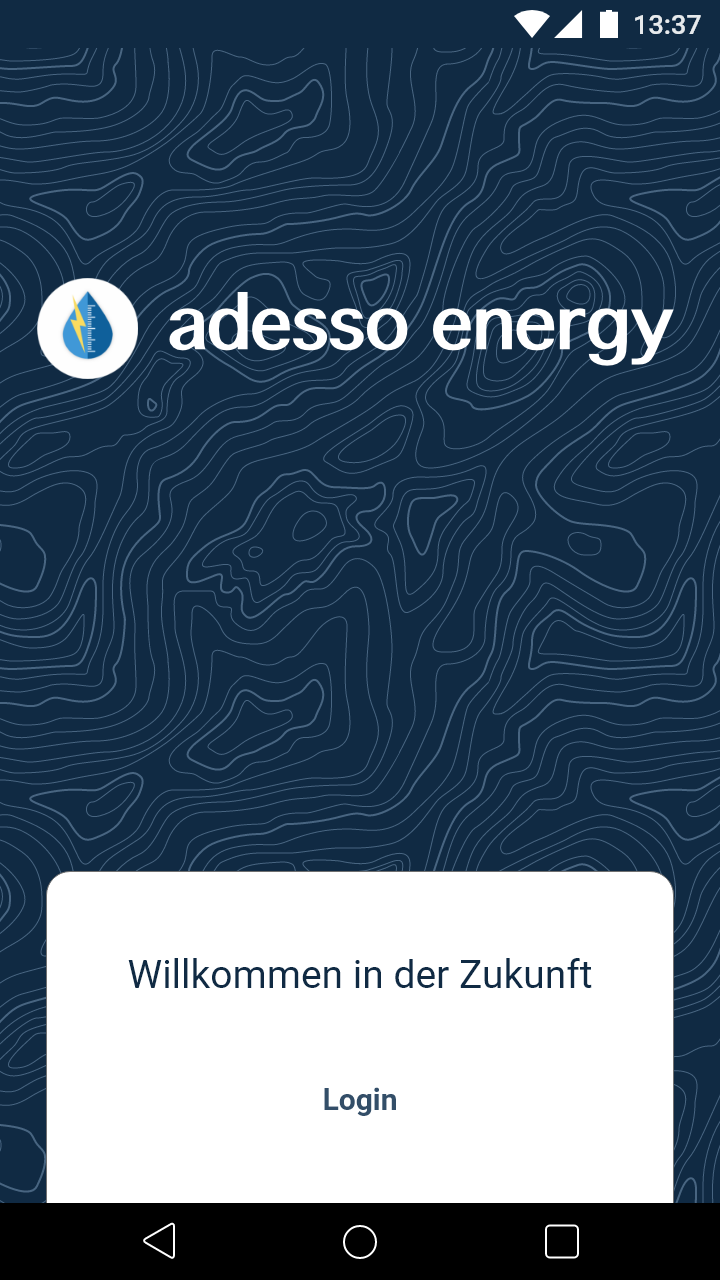
\includegraphics[scale = 0.155]{img/AndroidMockup/splash}  \caption {Startbildschirm} &  Dies ist der Bildschirm, den der Benutzer sieht, sobald er die App startet und noch nicht eingeloggt war.\\
	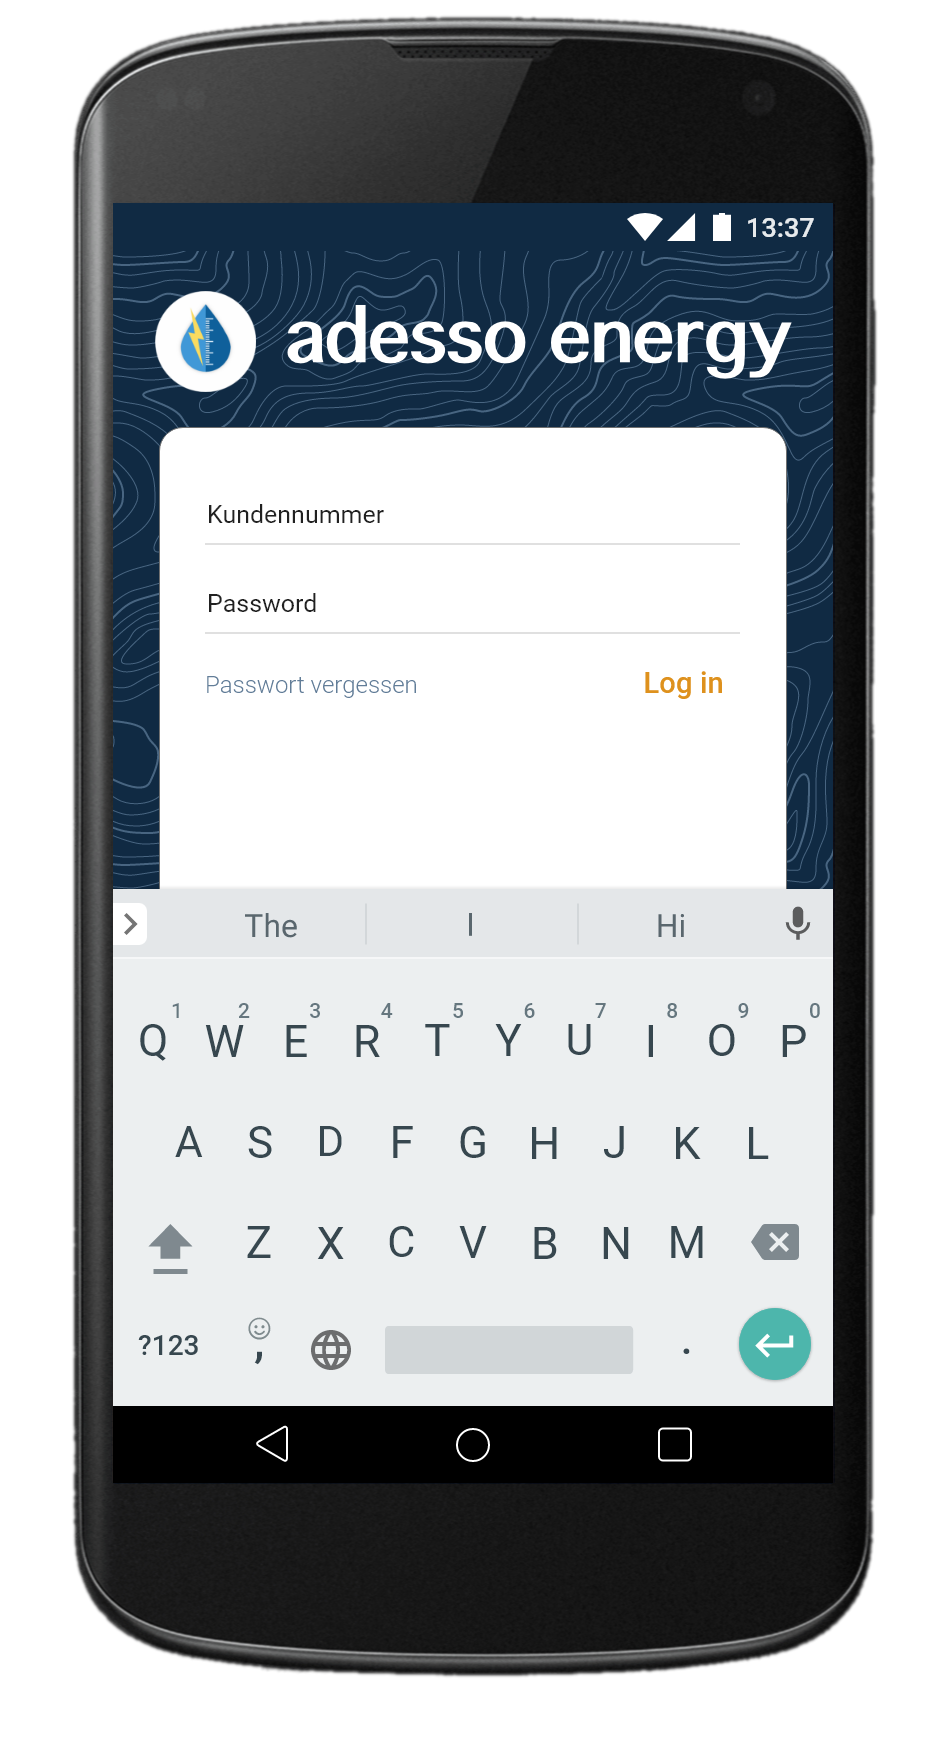
\includegraphics[scale = 0.155]{img/AndroidMockup/login} \caption {Anmeldebildschirm} &	Nachdem man auf dem Startbildschirm auf 'Log in' gedrückt hat, wird man auf den Anmeldebildschirm geleitet. Hier hat man die Möglichkeit, sich mit seiner Kundennummer und seinem Passwort einzuloggen. Außerdem hat man die Möglichkeit, mithilfe des 'Passwort vergessen'-Buttons, sein Passwort zurückzusetzen. \\ 
\end{tabularx}
\end{figure}


\begin{figure}[h]
\begin{tabularx}{\textwidth}{X  X}
	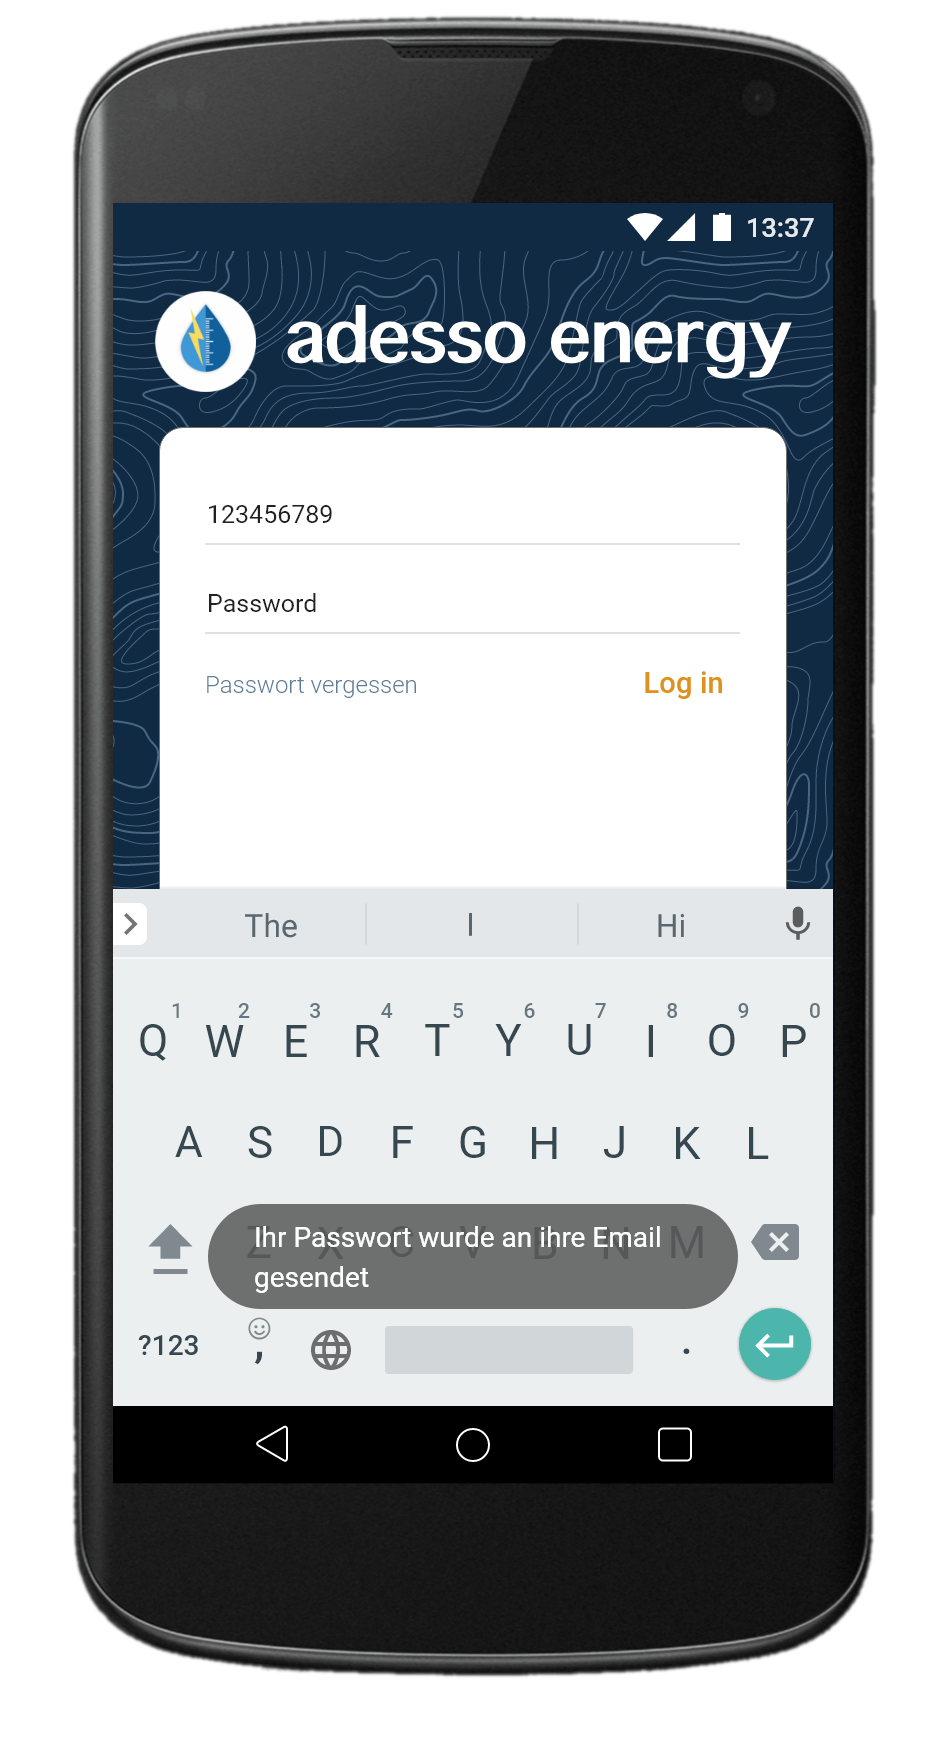
\includegraphics[scale = 0.155]{img/AndroidMockup/forgotPassword} \caption{Password vergessen} & Nachdem man auf 'Passwort vergessen' geklickt hat, erscheint eine Meldung, welche den Benutzer über das weitere Vorgehen informiert.\\
	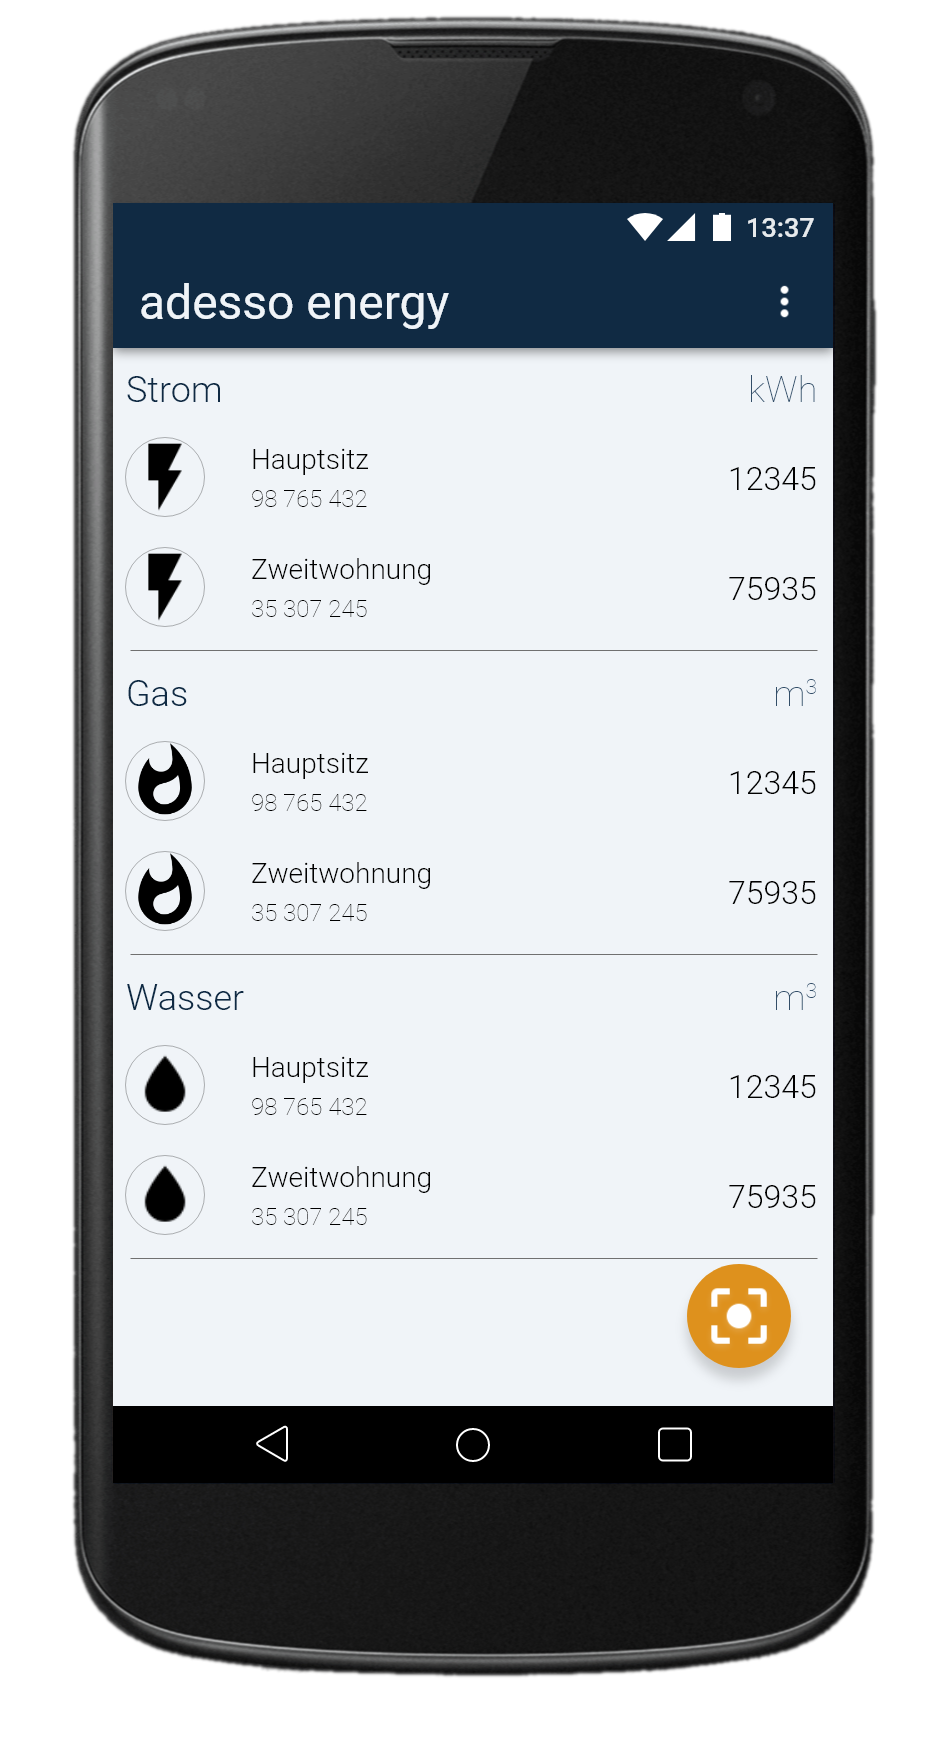
\includegraphics[scale = 0.155]{img/AndroidMockup/Main} \caption{Hauptbildschirm} & Nachdem man sich erfolgreich eingeloggt hat, landet man auf dem Hauptbildschirm. Hier sieht man eine Übersicht seiner Zähler mit deren Zählernummer und aktuellem Zählerstand. \\
\end{tabularx}
\end{figure}


\begin{figure}[h]
\begin{tabularx}{\textwidth}{X  X}
	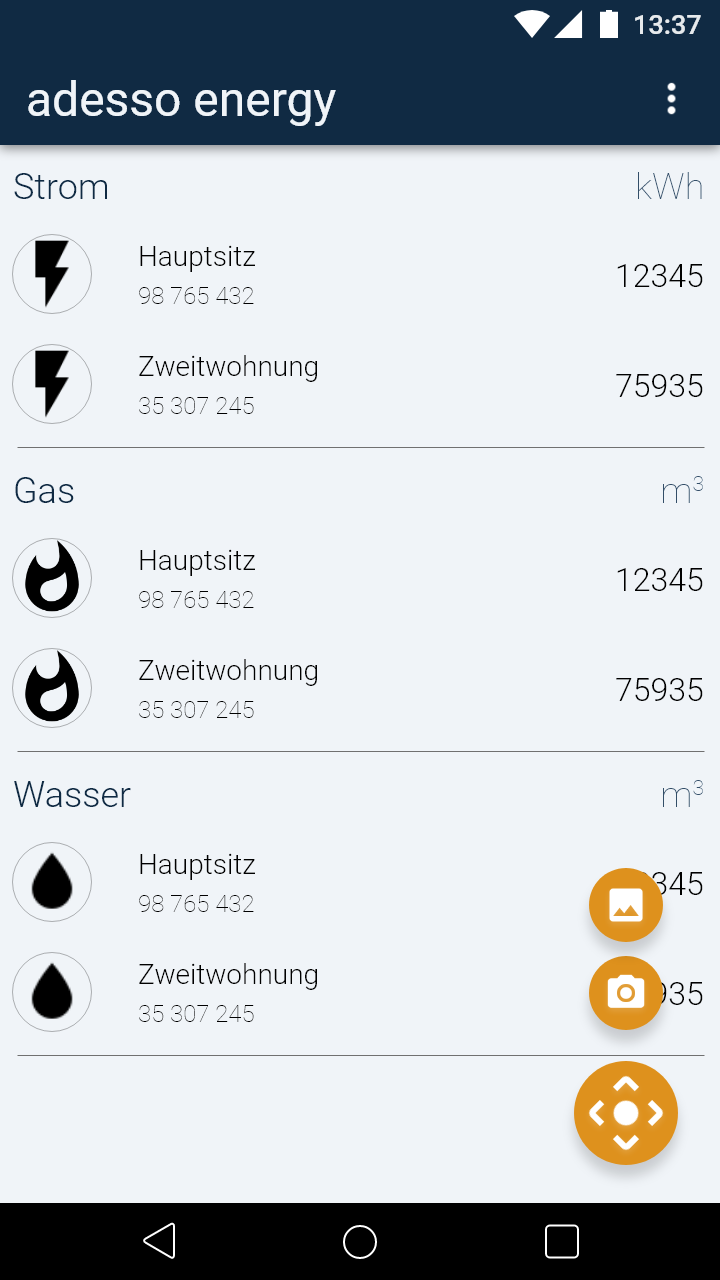
\includegraphics[scale = 0.155]{img/AndroidMockup/FABMenu} \caption{FAB-Menü}  & Klickt man auf den FAB, so erscheint ein Menü. Hier kann man sich entscheiden, ob man ein Bild aufnehmen möchte (Kamera-Symbol) oder eines aus der Galerie hochladen möchte (Galerie-Symbol). \\
	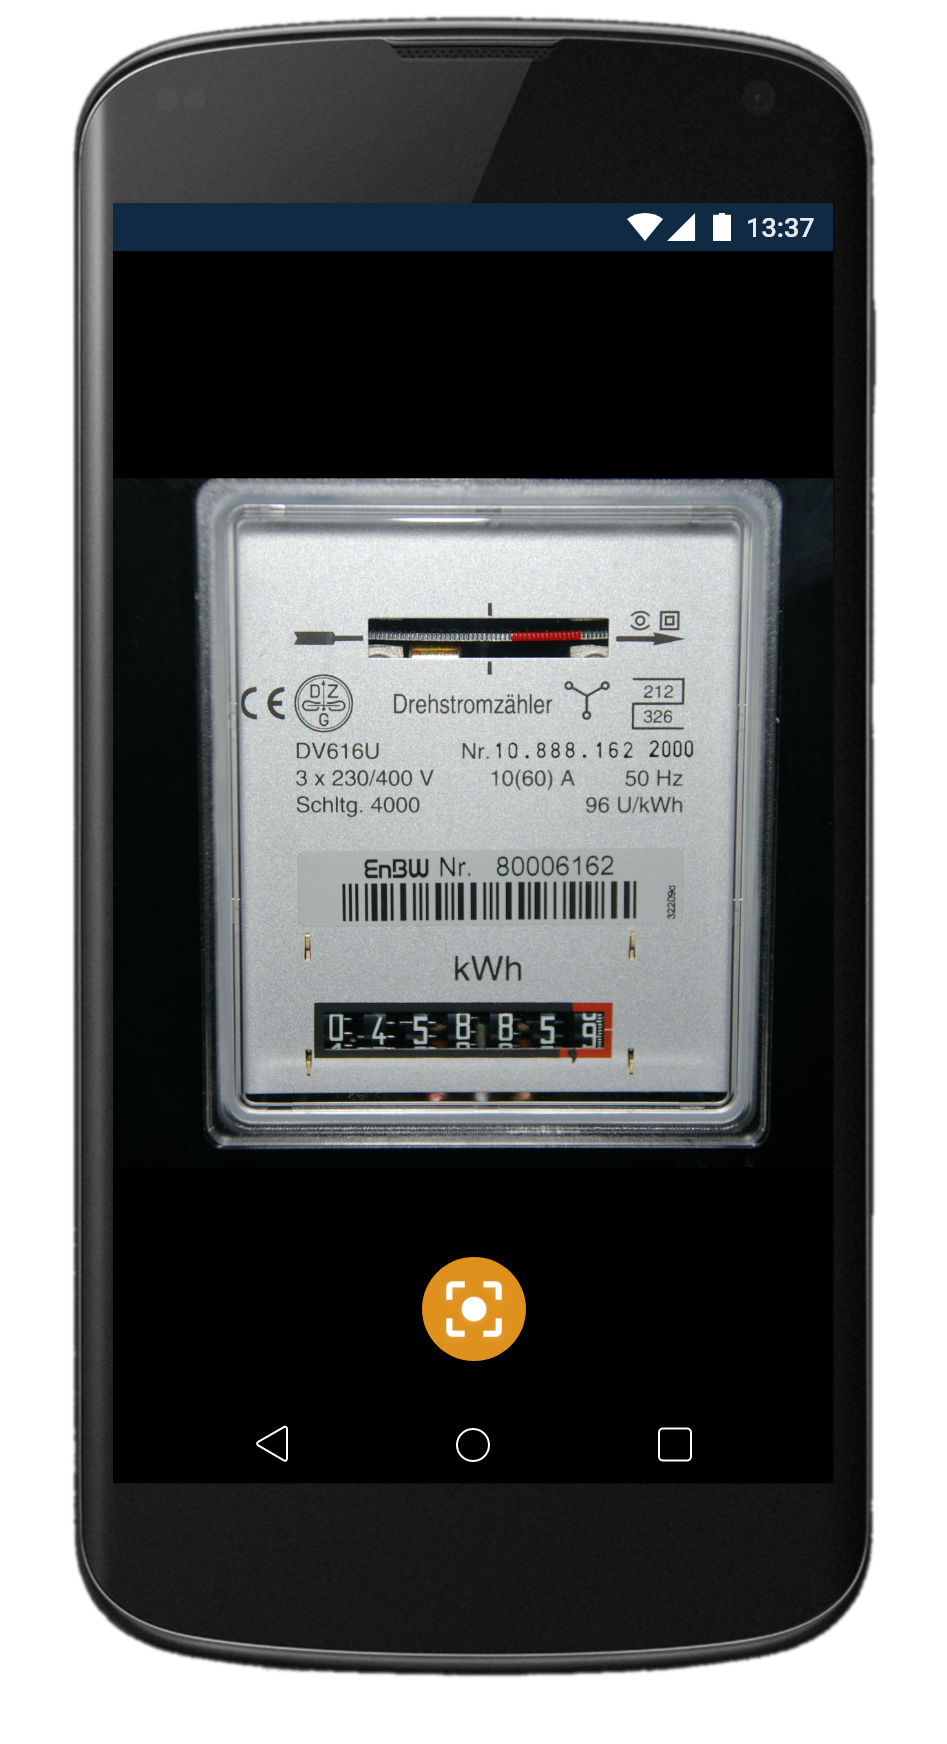
\includegraphics[scale = 0.155]{img/AndroidMockup/SystemCamera} \caption{Kamera-View}  & Nachdem man im Dropdown Menü das Kamera-Symbol gedrückt hat, öffnet sich die Kamera-App des Gerätes. \\ 
\end{tabularx}
\end{figure}

\begin{figure}[h]
\begin{tabularx}{\textwidth}{X  X}
	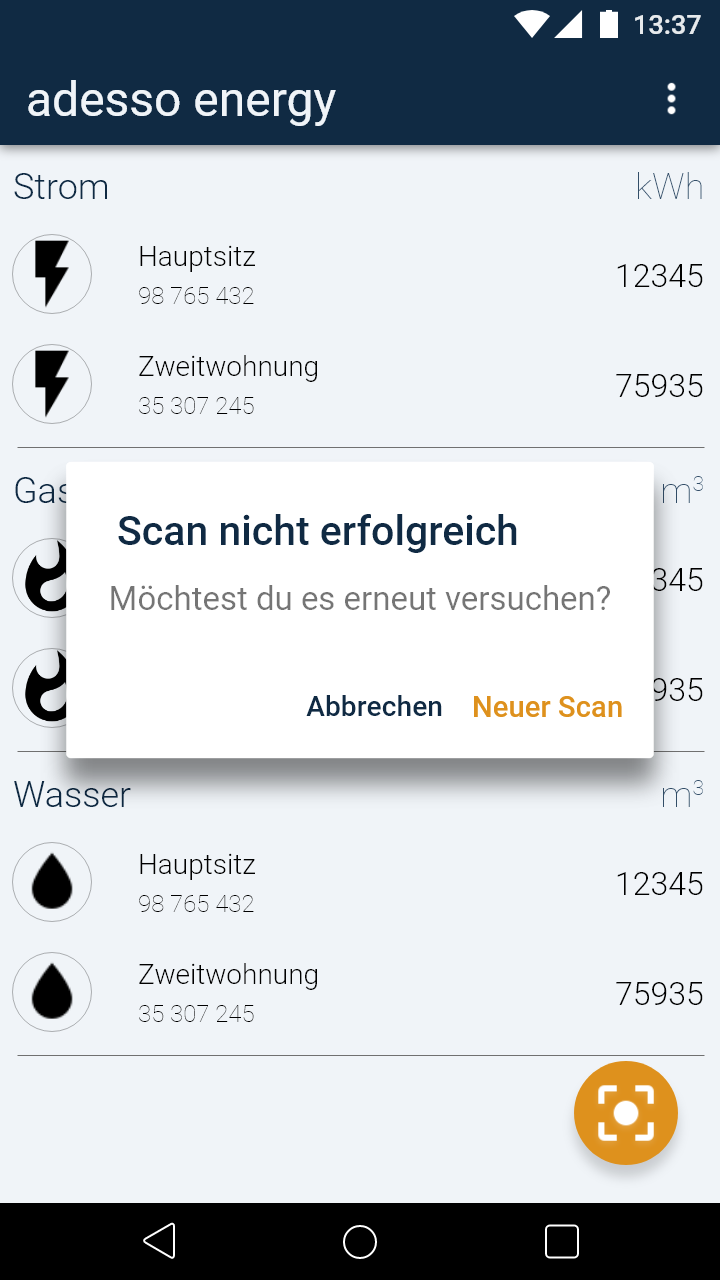
\includegraphics[scale = 0.155]{img/AndroidMockup/imageFailed} \caption{Scan fehlgeschlagen} & Wurde auf dem Bild kein Zähler erkannt, so erscheint eine entsprechende Meldung. Hier hat man die Möglichkeit, erneut ein Foto zu machen oder den Vorgang abzubrechen. \\
	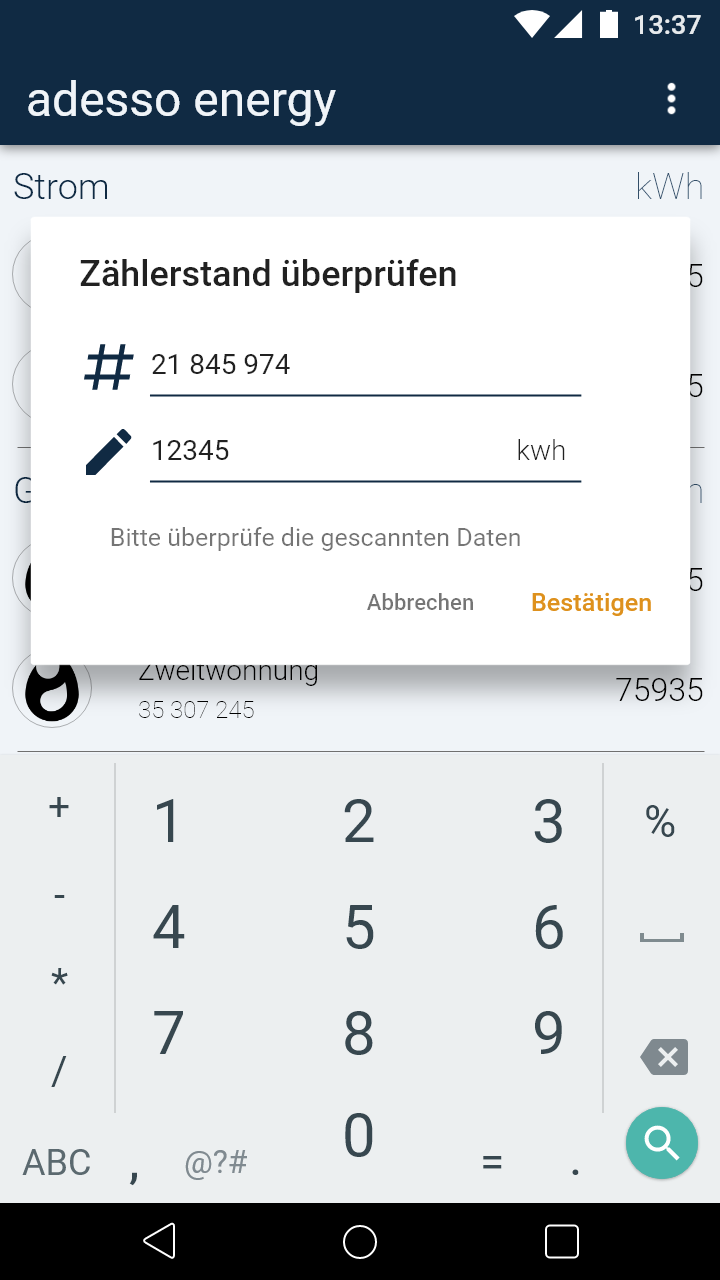
\includegraphics[scale = 0.155]{img/AndroidMockup/check} \caption{Werte überprüfen} & Wurde ein Foto erfolgreich verarbeitet, so folgt eine Überprüfung der Werte, welche von Azure erkannt wurden. Vor dem endgültigen Speichern der Werte müssen diese vom Benutzer bestätigt werden. \\ 
\end{tabularx}
\end{figure}

\begin{figure}[h]
\begin{tabularx}{\textwidth}{X  X}
	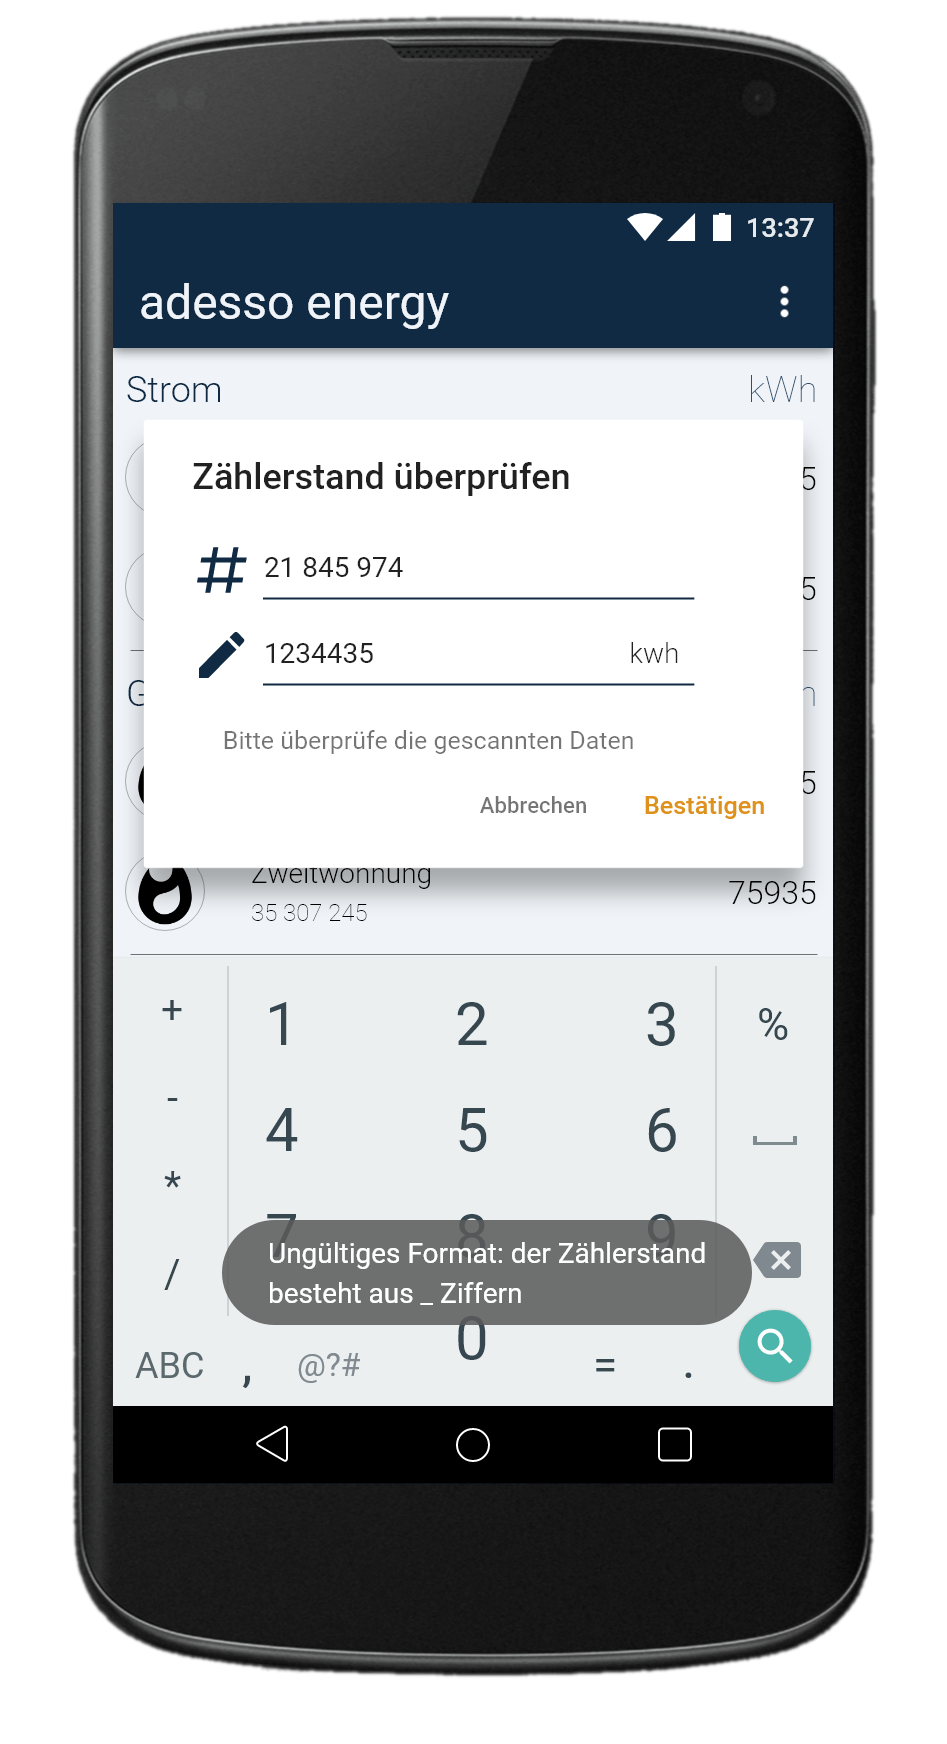
\includegraphics[scale = 0.155]{img/AndroidMockup/illegalFormatException} \caption{Falsches Zahlenformat} & Gibt man Werte in einem falschem Format ein, so erhält man eine entsprechende Meldung. \\
	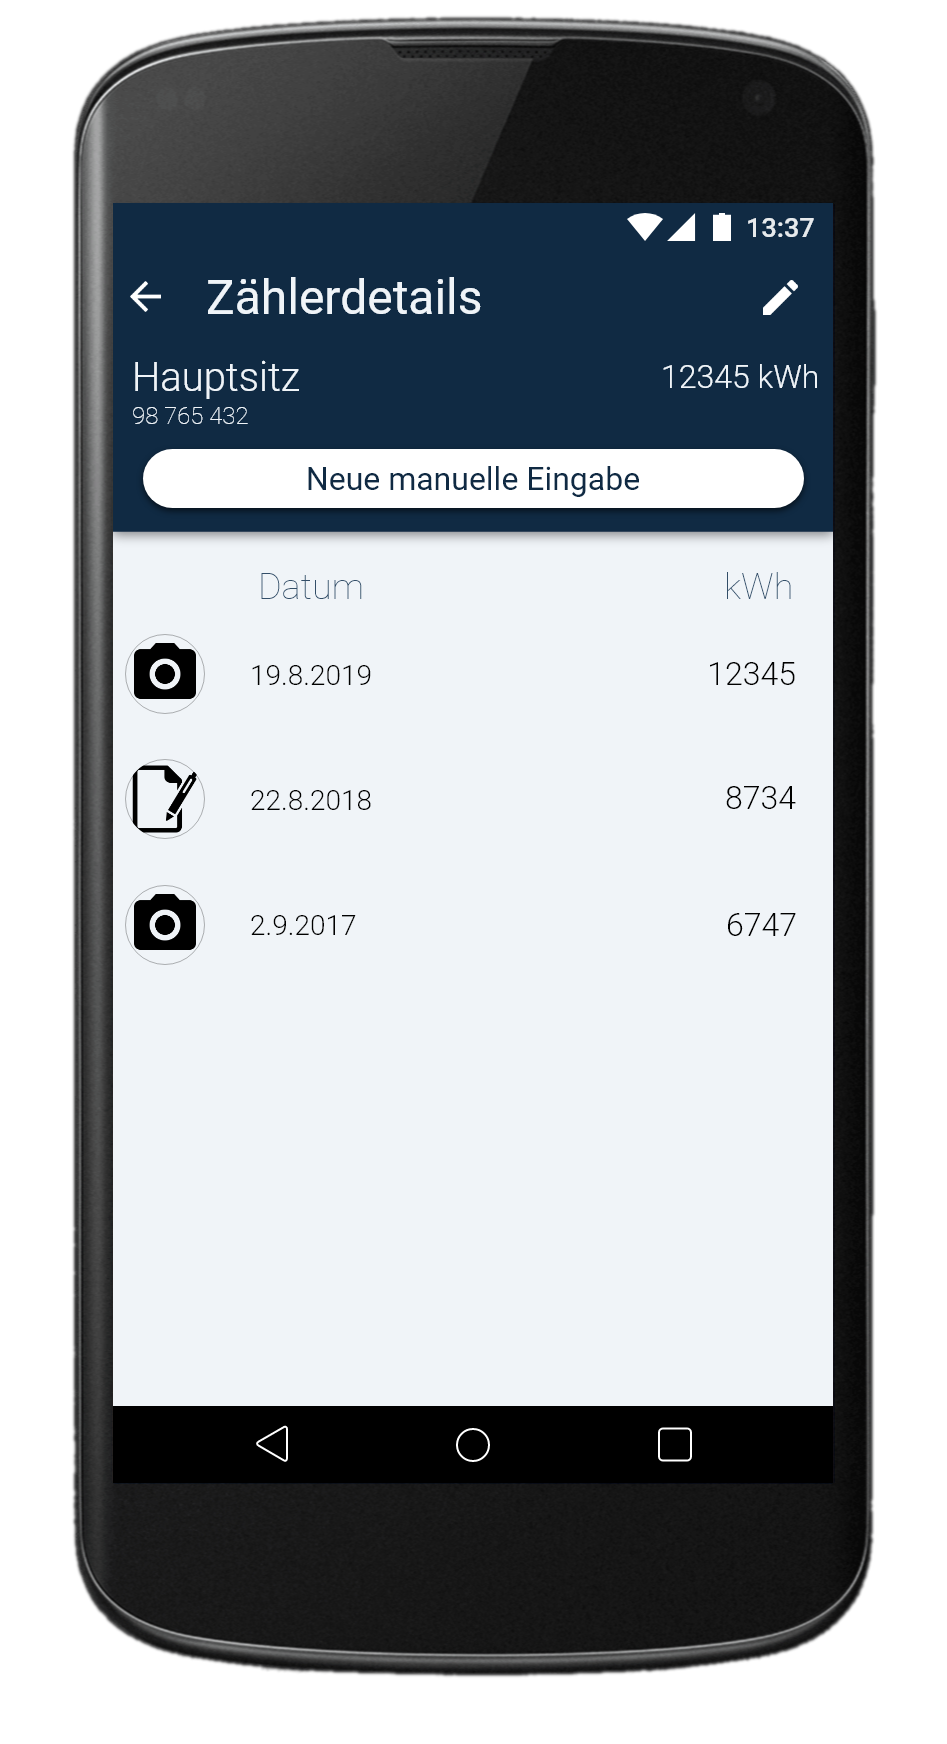
\includegraphics[scale = 0.155]{img/AndroidMockup/history} \caption{Zählerstand-Details} & Klickt man auf einen der Zähler, so sieht man die gesamte History der eingetragenen Zählerstände. Außerdem sieht man, wann der Zählerstand hochgeladen worden ist und ob dies durch eine manuelle Eingabe oder per Foto geschah. \\
\end{tabularx}
\end{figure}

\begin{figure}[h]
\begin{tabularx}{\textwidth}{X  X}
	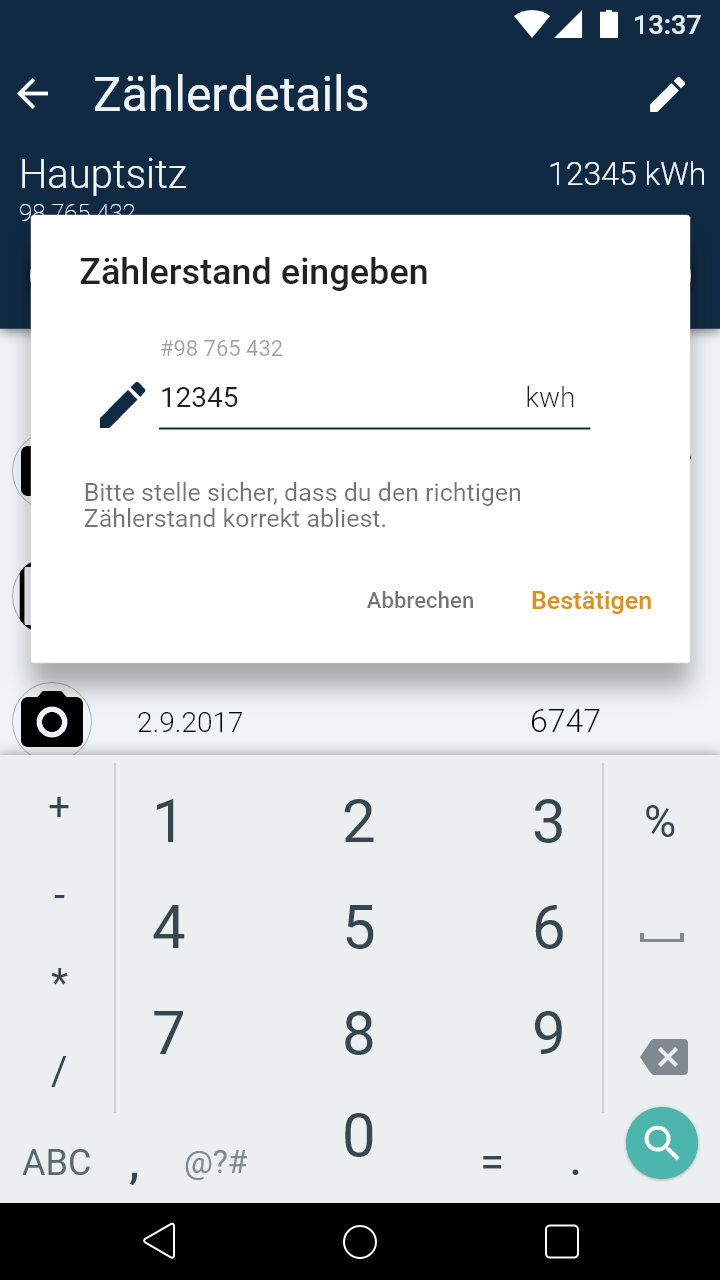
\includegraphics[scale = 0.155]{img/AndroidMockup/manuelEntry} \caption{Manueller Eintrag}&  Sobald der Zähler ausgewählt ist, hat man die Möglichkeit, manuell einen Zählerstand einzutragen. \\
	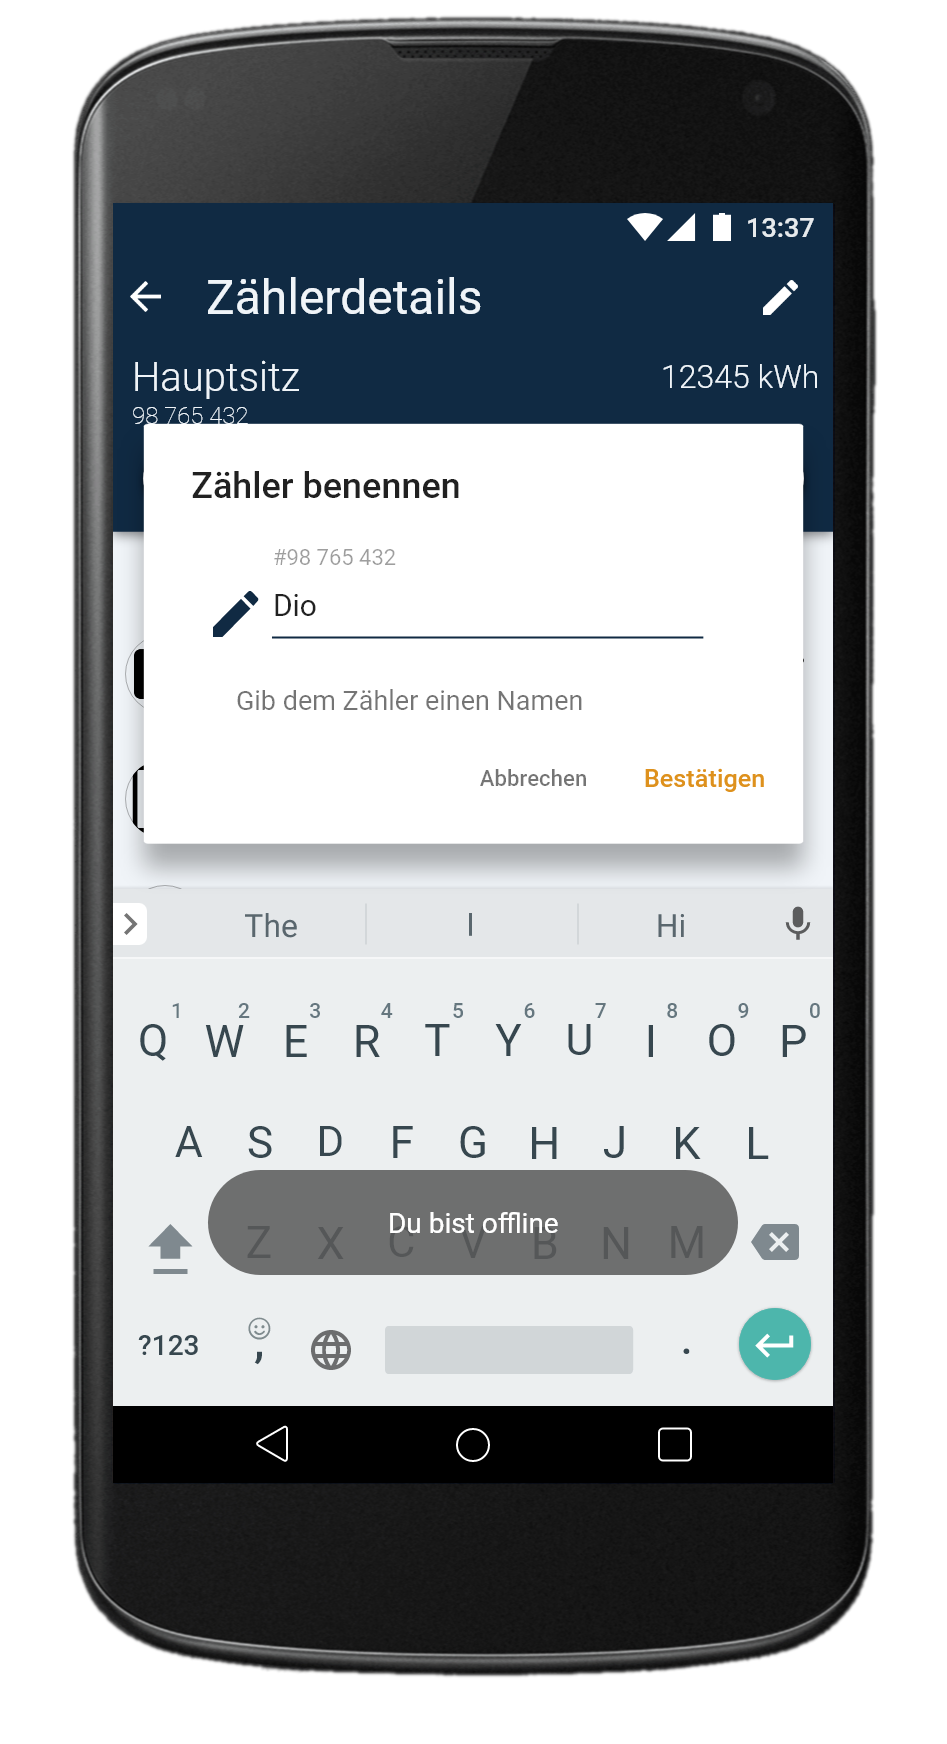
\includegraphics[scale = 0.155]{img/AndroidMockup/renameException} \caption{Offline-Meldung} & Verliert man während eines Vorganges seine Internetverbindung, so erscheint eine entsprechende Meldung und der Vorgang wird nicht durchgeführt.  \\ 
\end{tabularx}
\end{figure}

\begin{figure}[h]
\begin{tabularx}{\textwidth}{X  X}
	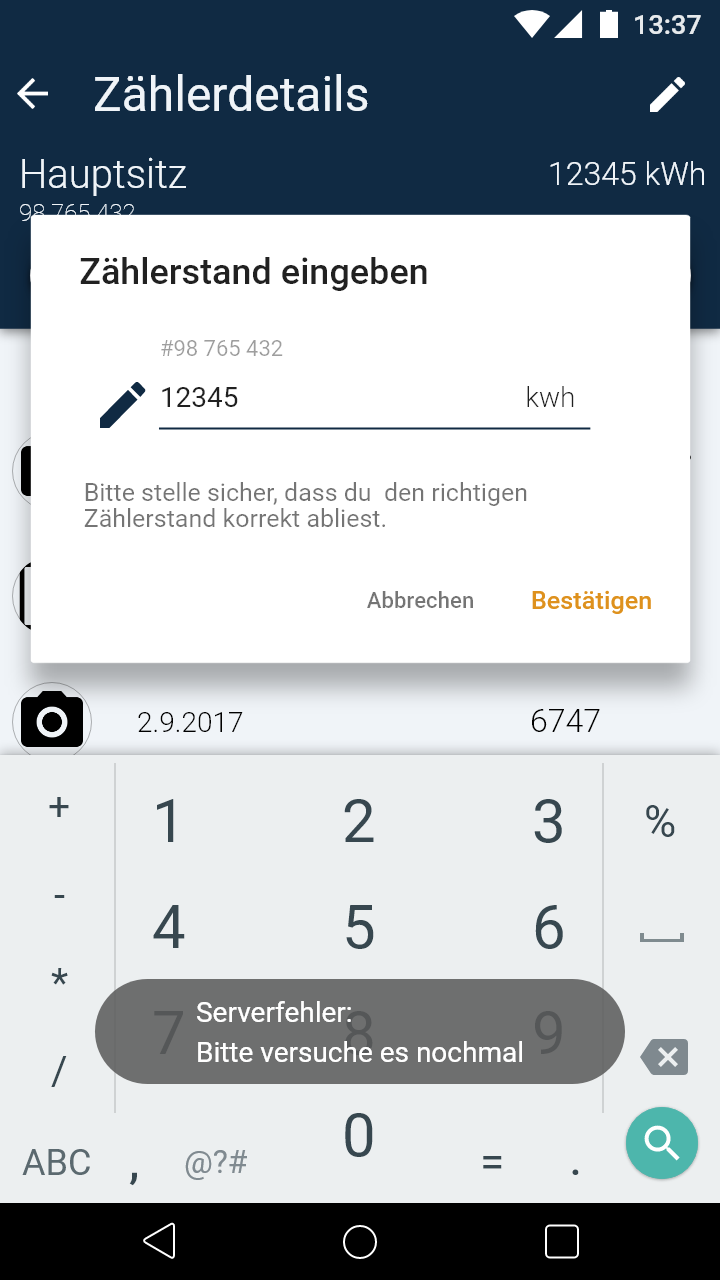
\includegraphics[scale = 0.155]{img/AndroidMockup/serverException} \caption{Serverfehler} & Falls während der Ausführung eines Vorganges ein Serverproblem geschieht, so erscheint eine entsprechende Meldung und der Vorgang wird nicht durchgeführt.\\
	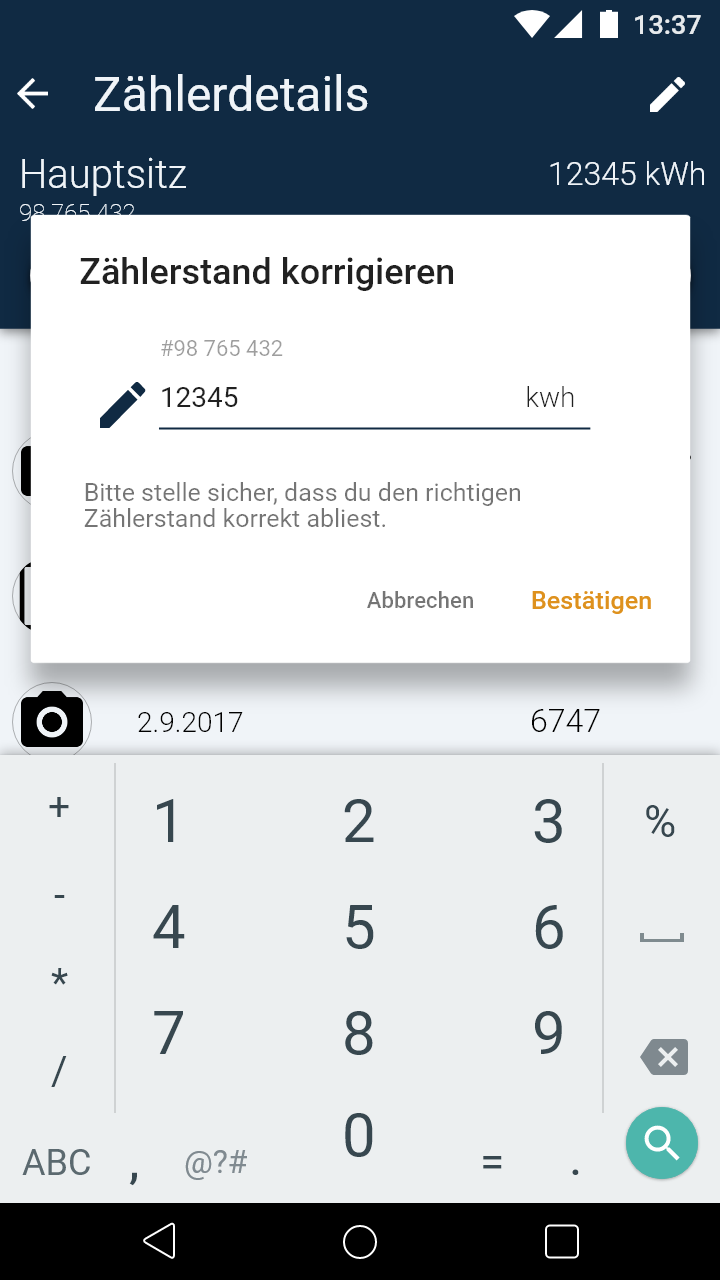
\includegraphics[scale = 0.155]{img/AndroidMockup/correct} \caption{Zählerstand korrigieren} & Wurde ein falscher Zählerstand eingetragen, so hat man nachträglich die Möglichkeit, ihn zu korrigieren.\\ 
\end{tabularx}
\end{figure}

\begin{figure}[h]
\begin{tabularx}{\textwidth}{X  X}
	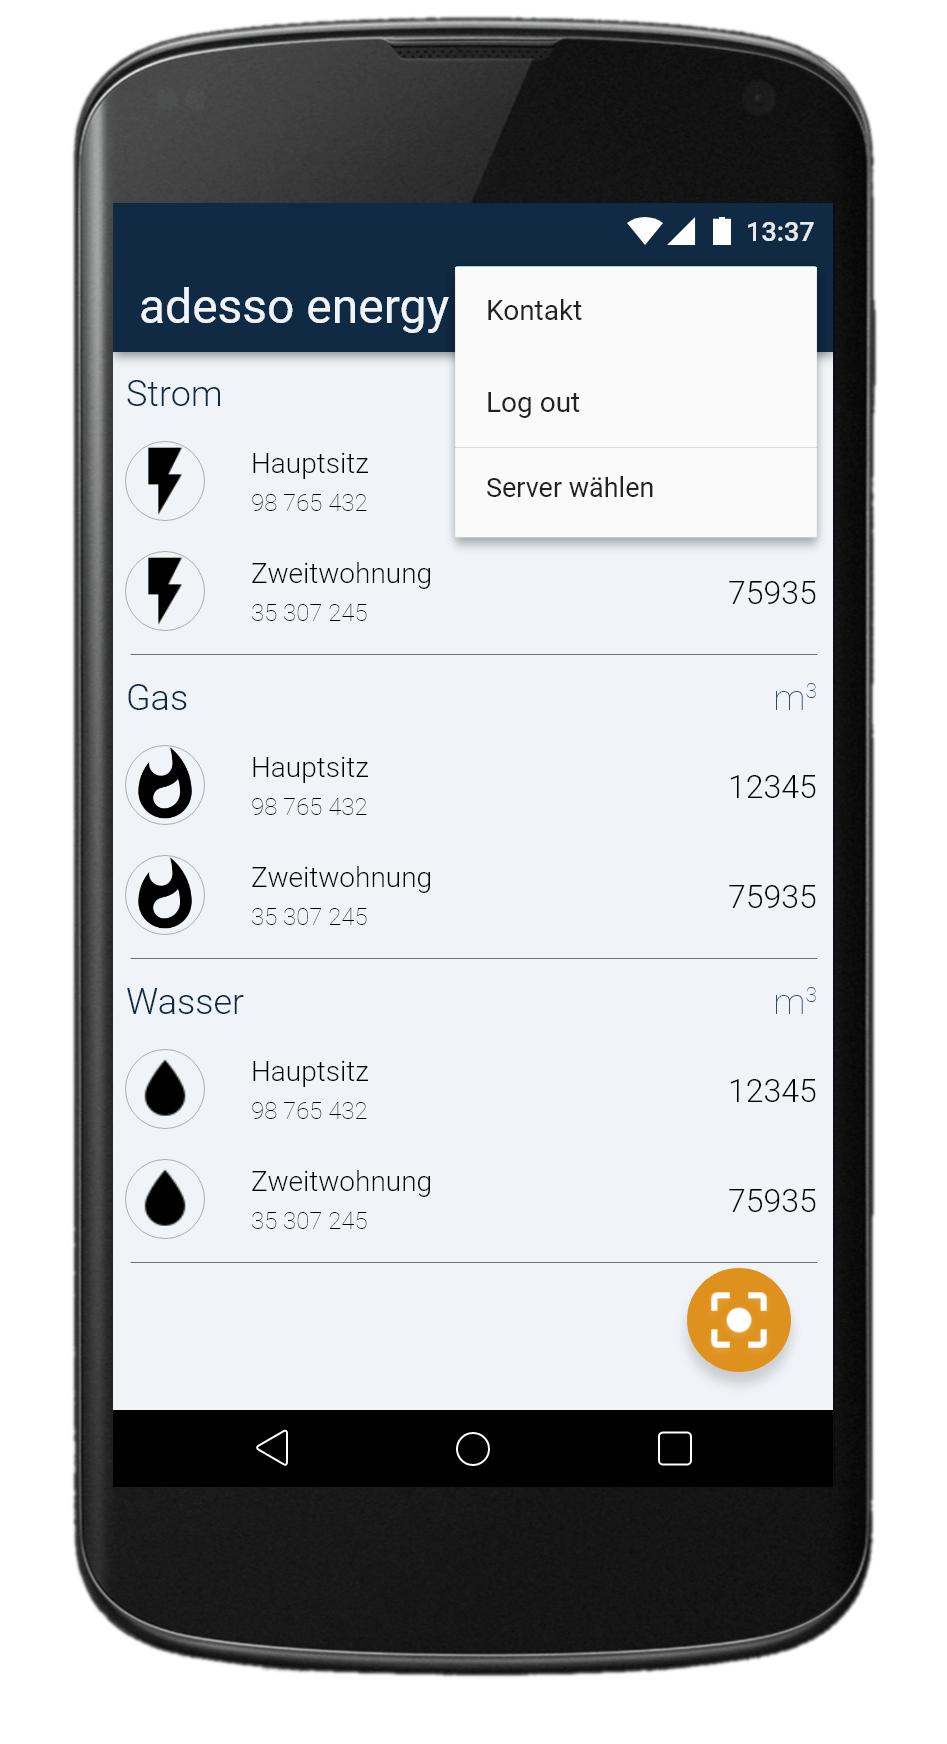
\includegraphics[scale = 0.155]{img/AndroidMockup/dropdown} \caption{Dropdown-Menü} & Man hat auf dem Startbildschirm außerdem die Möglichkeit, oben rechts ein Dropdown-Menü zu öffnen. Hier hat man die Möglichkeit, die Adresse des Servers auszuwählen, sich abzumelden, sowie Kontakt zum Support aufzunehmen. \\
	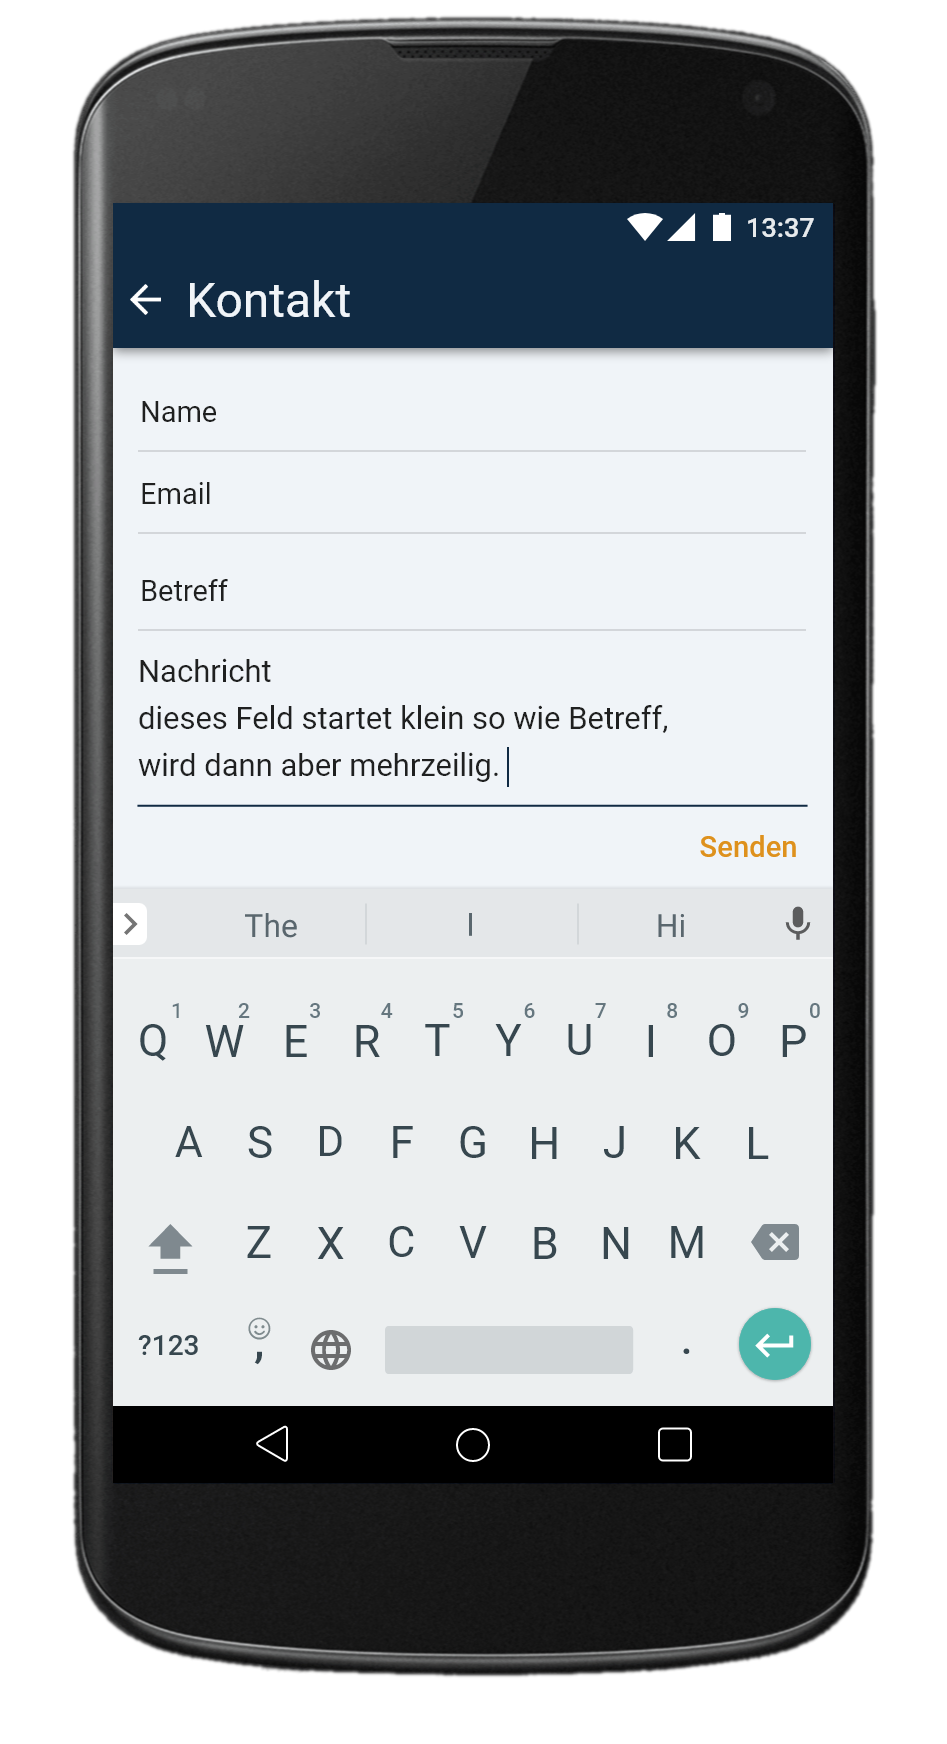
\includegraphics[scale = 0.155]{img/AndroidMockup/contact} \caption{Kontaktformular} & Sobald man sich entschieden hat, Kontakt mit dem Support aufzunehmen, erscheint ein Kontaktformular. Hier soll der Benutzer seinen Namen, seine e-Mail-Adresse, den Betreff und eine Nachricht angeben. \\ 
\end{tabularx}
\end{figure} 

\begin{figure}[h]
\begin{tabularx}{\textwidth}{X  X}
	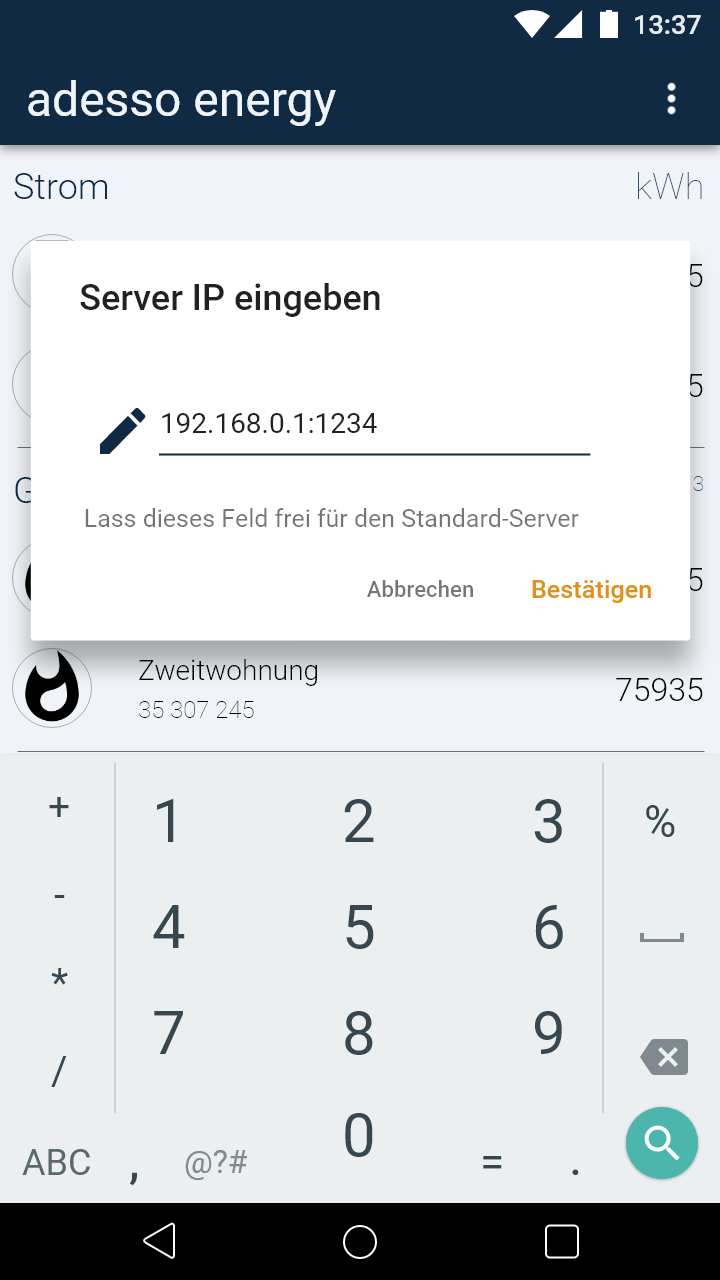
\includegraphics[scale = 0.155]{img/AndroidMockup/serverLocation} \caption{Server wählen} & Möchte man die Adresse des Servers ändern, so klickt man auf 'Server wählen'. Hier hat man die Möglichkeit, einen Servers mithilfe seiner IP-Adresse zu bestimmen und auf diesen zu wechseln. \\
	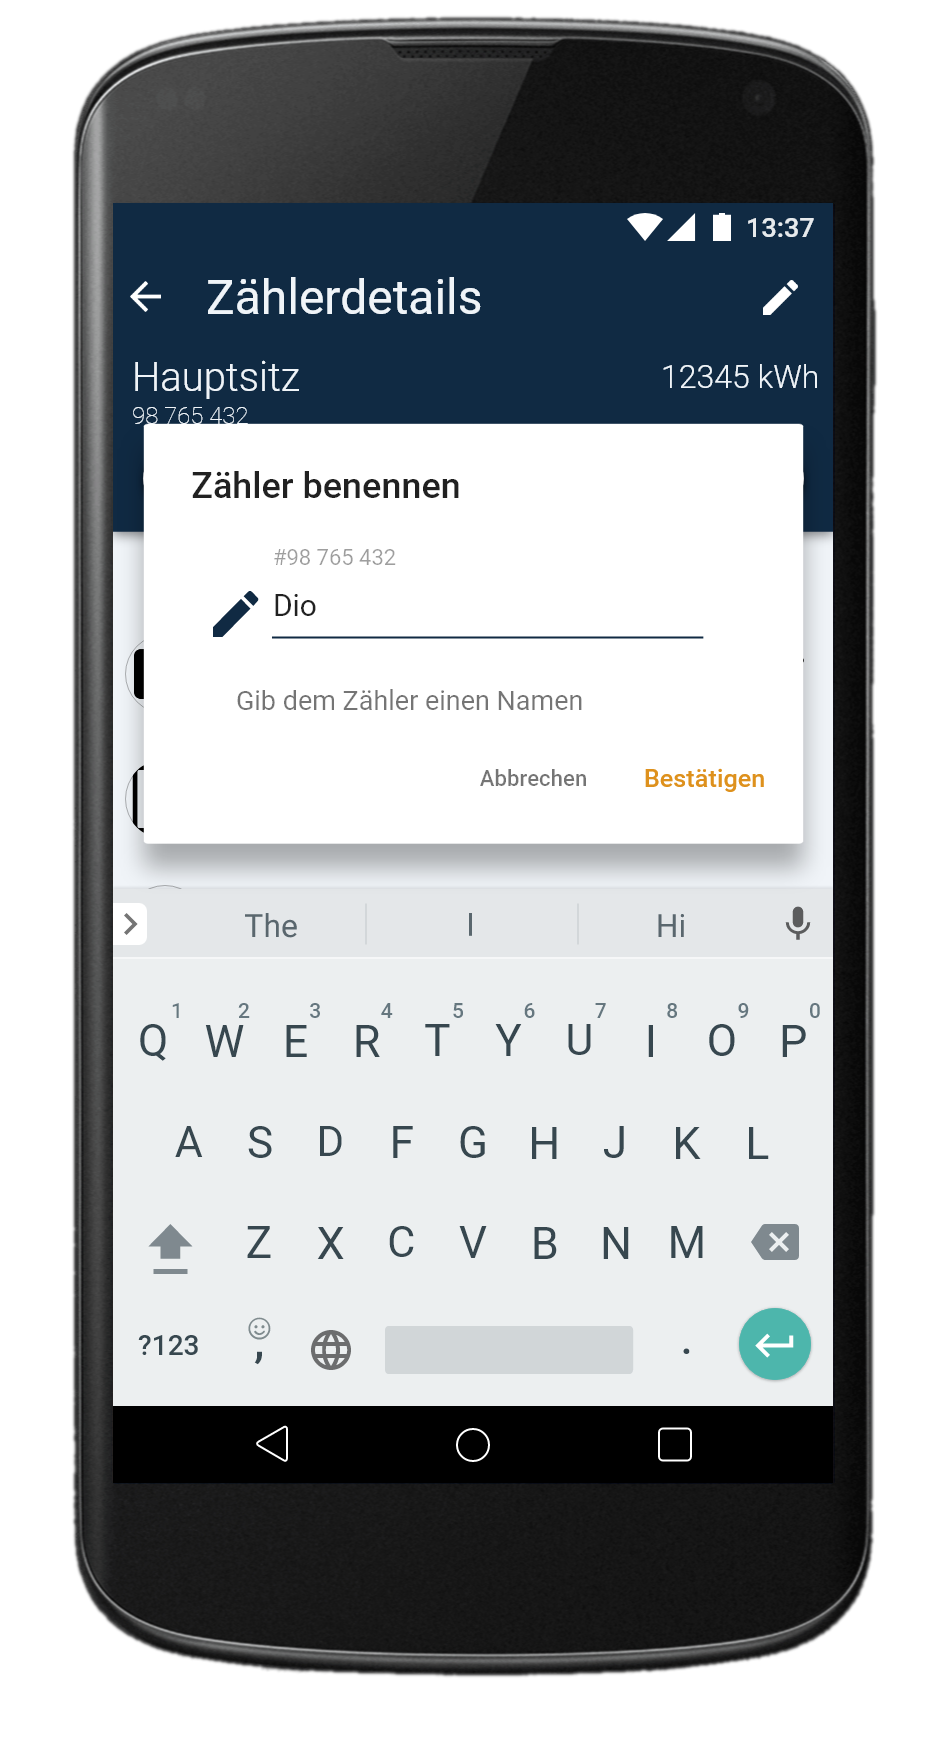
\includegraphics[scale = 0.155]{img/AndroidMockup/rename} \caption{Zähler umbenennen} & Wenn der Benutzer einen Zähler aus dem Hauptbildschirm ausgewählt hat, hat er die Möglichkeit, diesem zur einfacheren Identifikation einen Namen zuzuweisen. \\
\end{tabularx}
\end{figure}

% Section Web

\newpage

\begin{figure}[h] 
	\newpage
	\section{Web Mockup}

	In diesem Abschnitt werden die Mockups der Webseite vorgestellt, welche in interaktiver Form auch hier zu finden sind:
	\url{https://www.figma.com/file/Eyt5hgvjWapVjybG8g21tF/Website?node-id=0%3A1} .

	\centering
    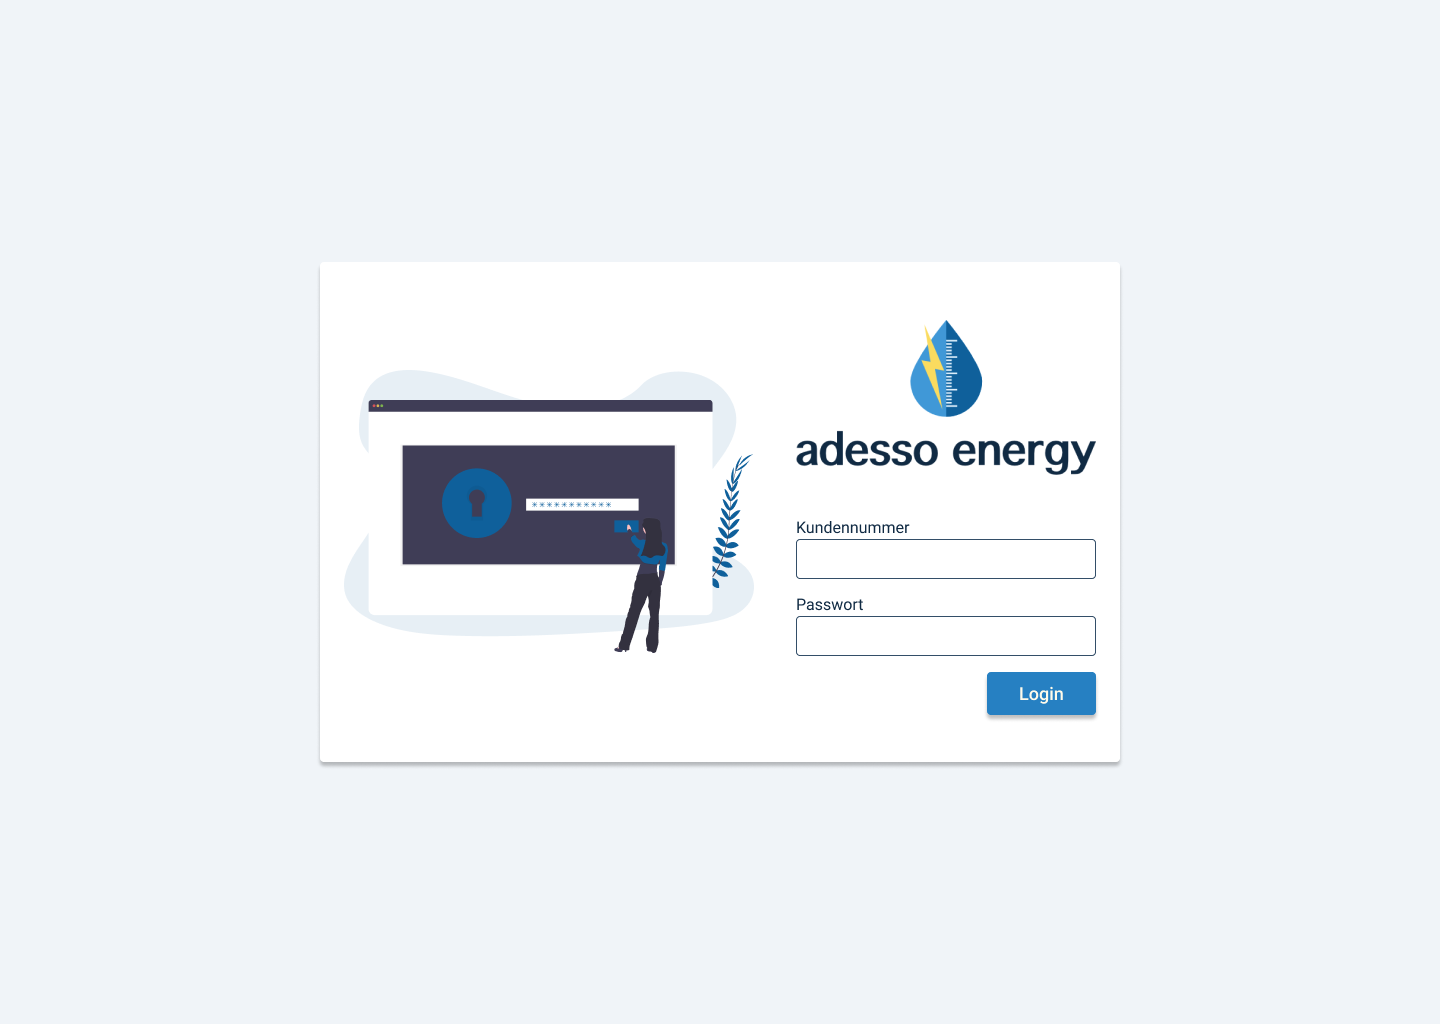
\includegraphics[scale=0.3]{img/WebsiteMockup/Login-User}
	\caption{Login Bildschirm} \hfill \break
	Hier sieht man den Login Screen in dem sich User und Admins mithilfe von Kundennummer und Passwort anmelden kann.
\end{figure}
 
\newpage

\begin{figure}[h]
	\centering
    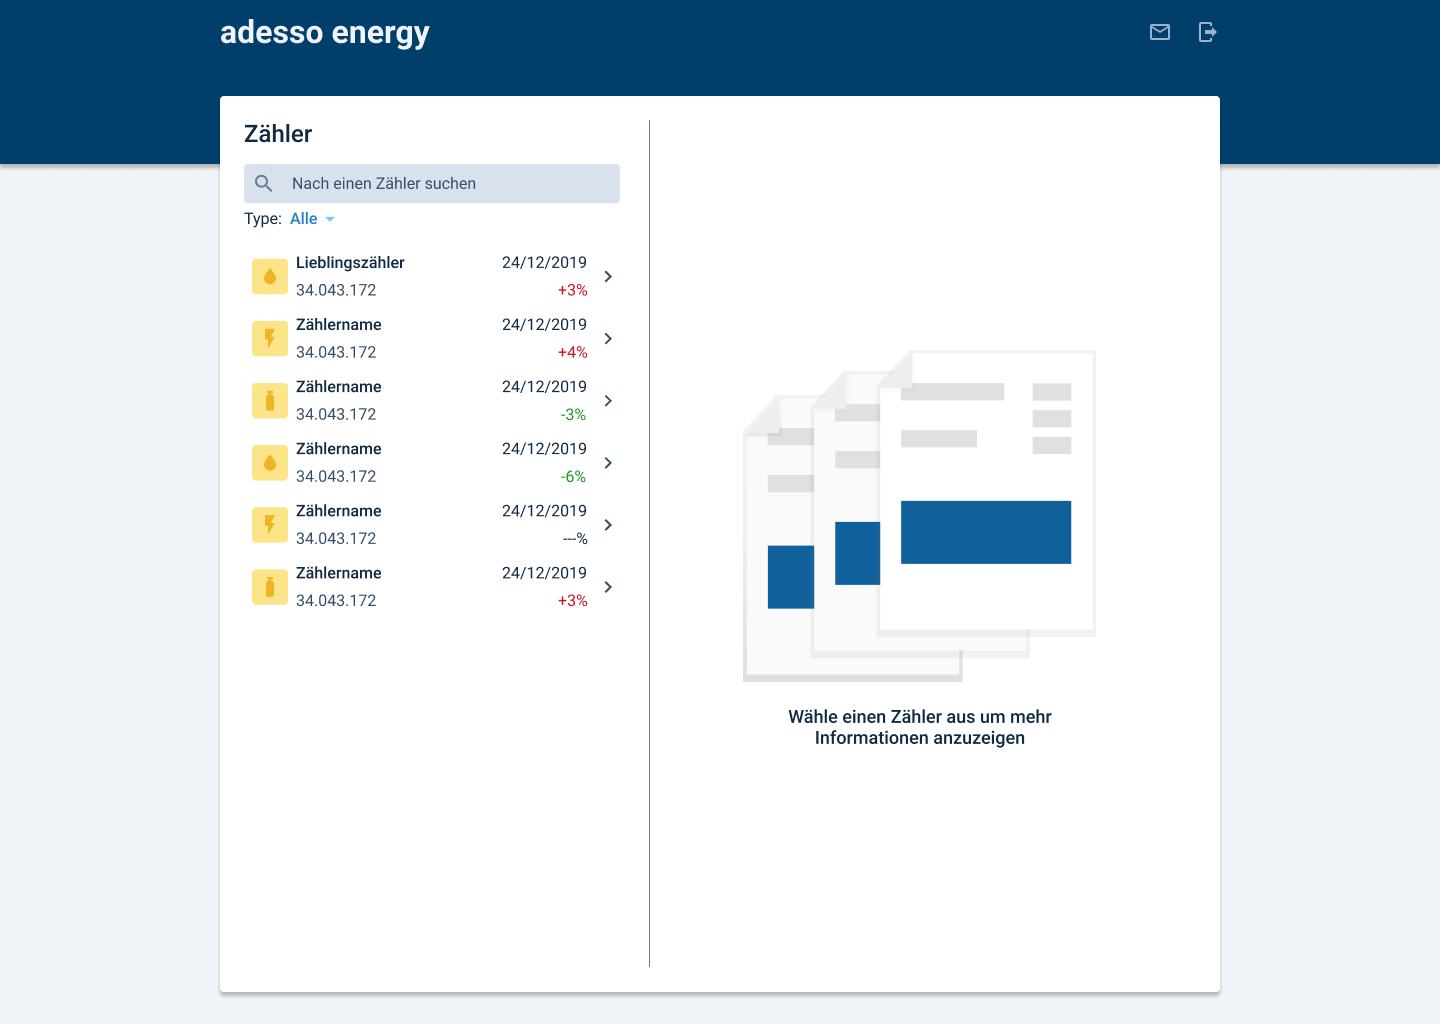
\includegraphics[scale=0.3]{img/WebsiteMockup/Dashboard-User-NonSelected}
	\caption{Dashboard User} \hfill \break
	Nachdem man sich erfolgreich eingeloggt wird man auf den Startbildschirm weitergeleitet. Hier kann der Benutzer seine Zähler einsehen.
\end{figure}

\newpage

\begin{figure}[h]
	\centering
    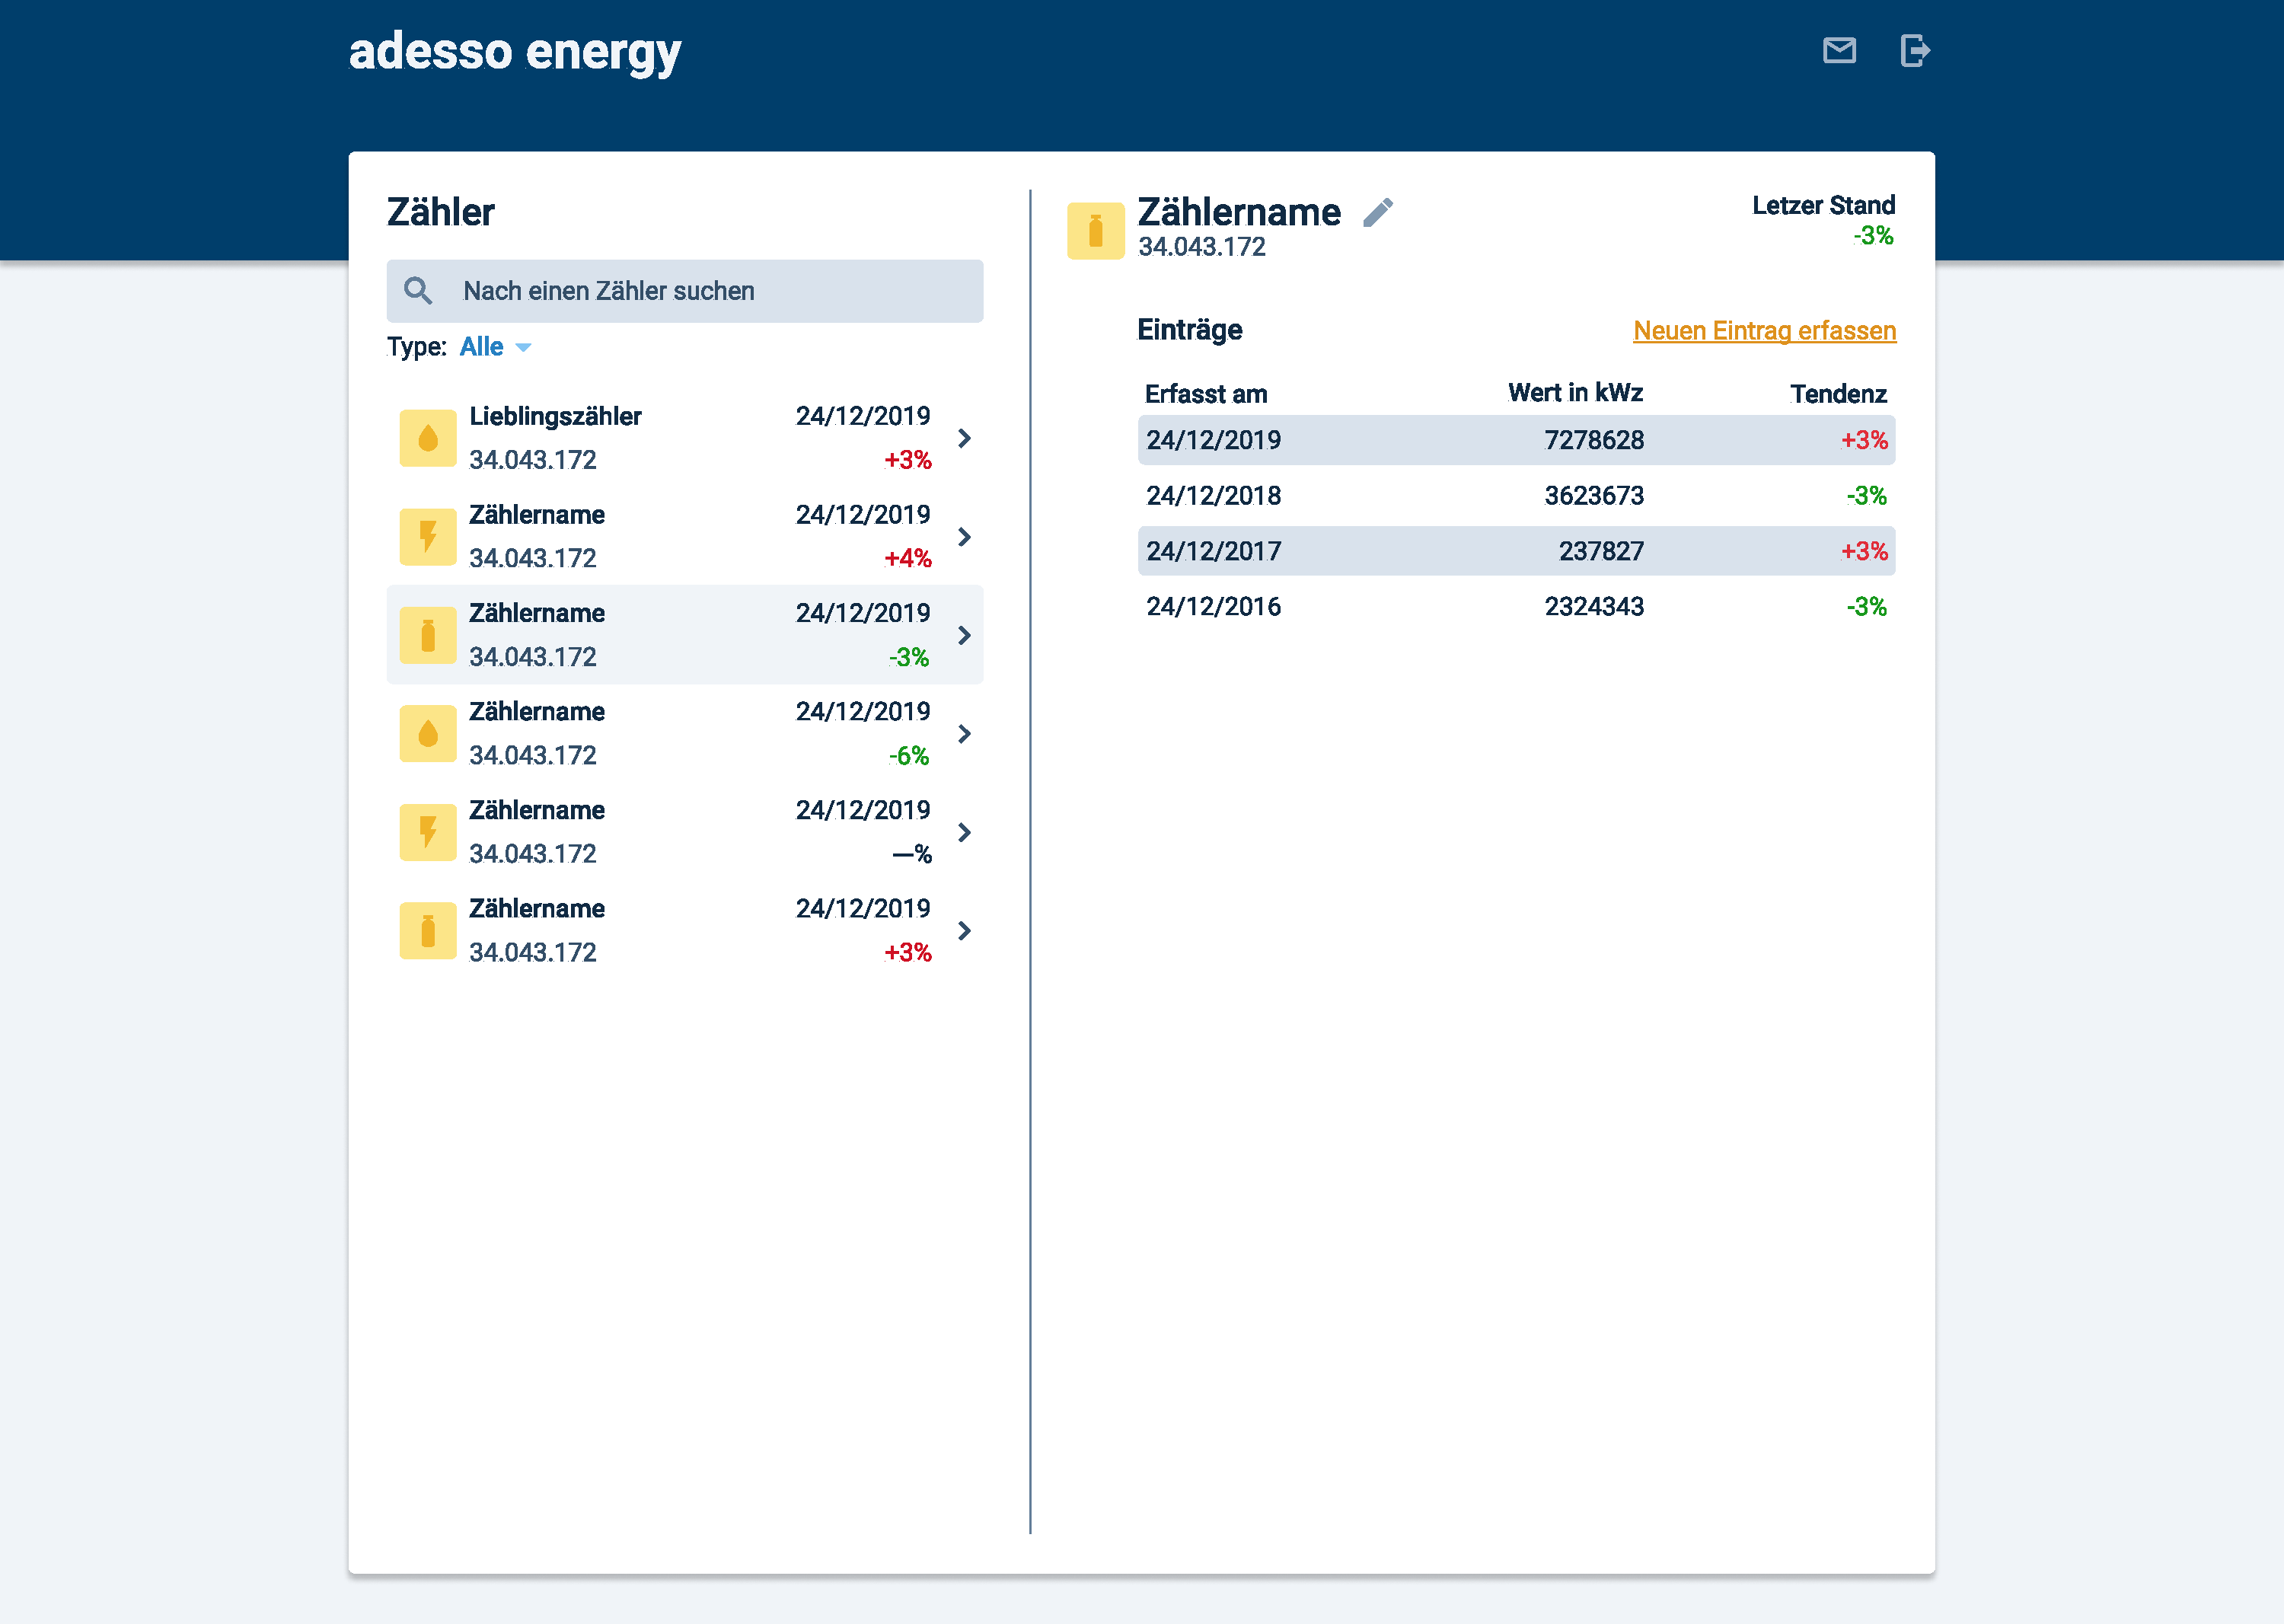
\includegraphics[scale=0.3]{img/WebsiteMockup/Dashboard-User-Selected}
	\caption{Dashboard User mit ausgewähltem Zähler} \hfill \break
	Nachdem man einen Zähler ausgewählt hat, sieht man seine History mit Datum und Zählerstand.
\end{figure}

\newpage

\begin{figure}[h]
	\centering
    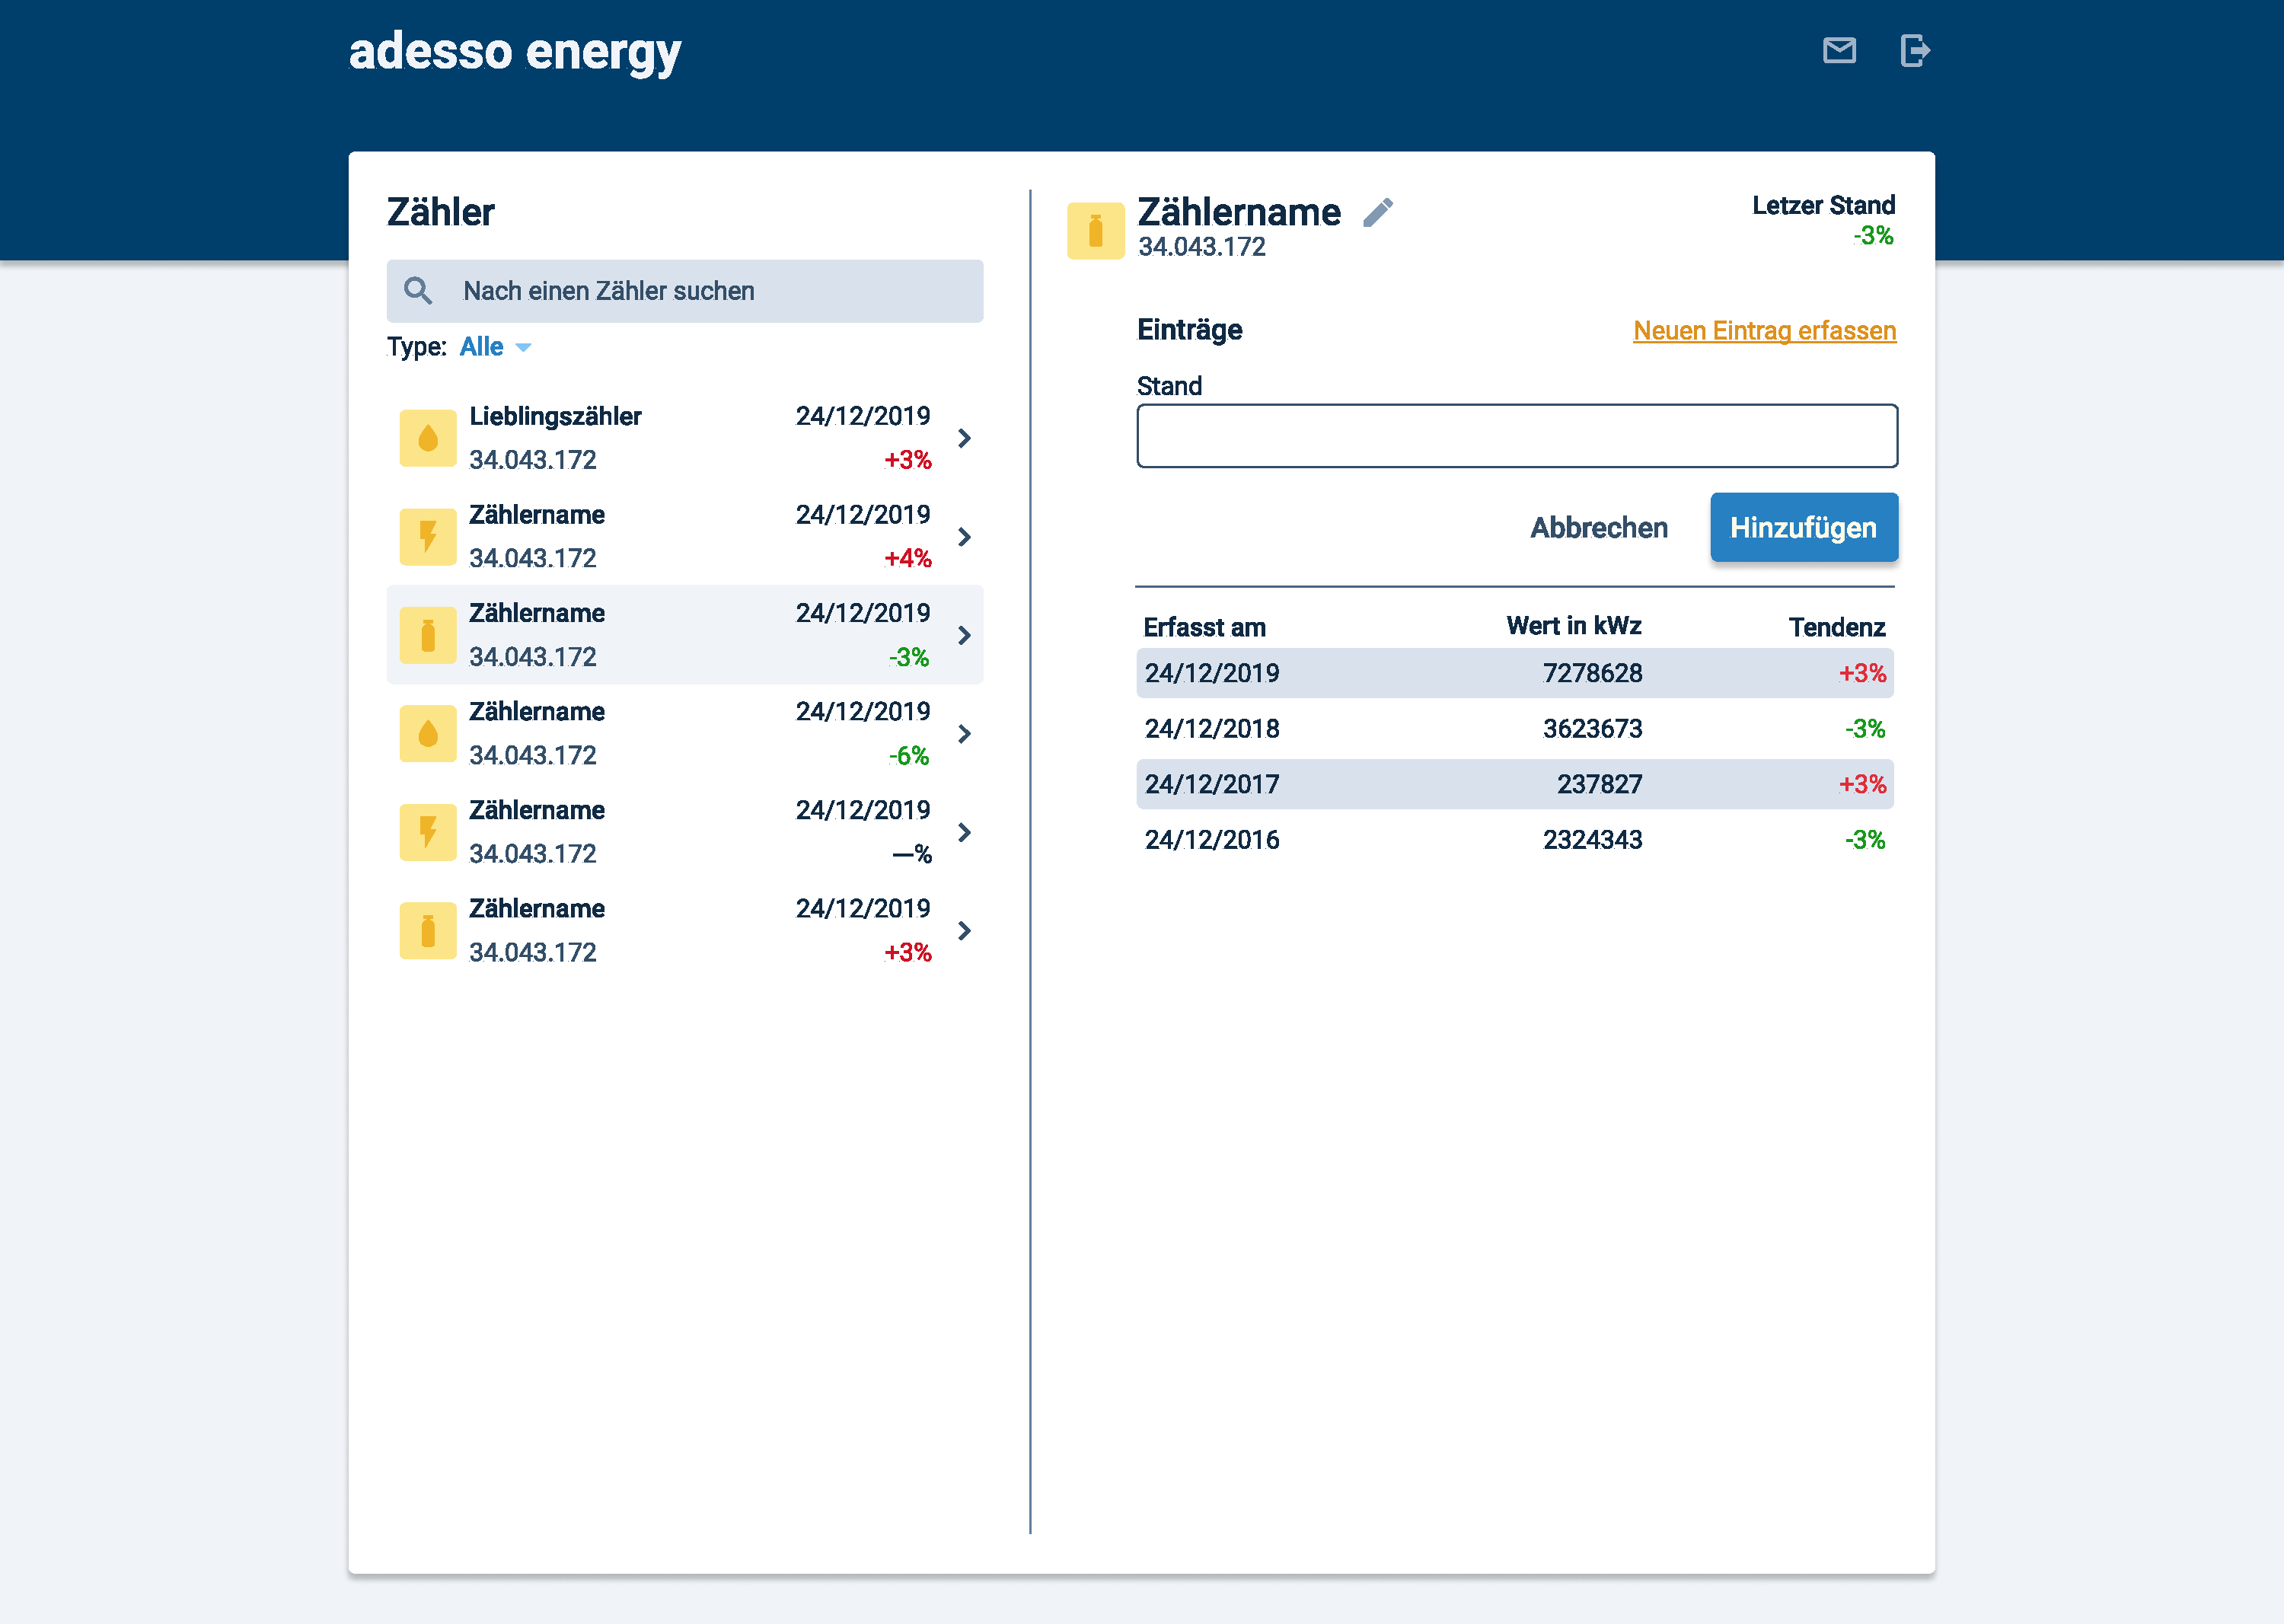
\includegraphics[scale=0.3]{img/WebsiteMockup/Dashboard-User-Selected-AddEntry}
	\caption{Dashboard User Eintrag hinzufügen} \hfill \break
	Nachdem man auf Neuen Eintrag erfassen klickt, wird ein Dialog angezeigt um einen neuen Stand festzuhalten.
\end{figure}

\newpage

\begin{figure}[h]
	\centering
    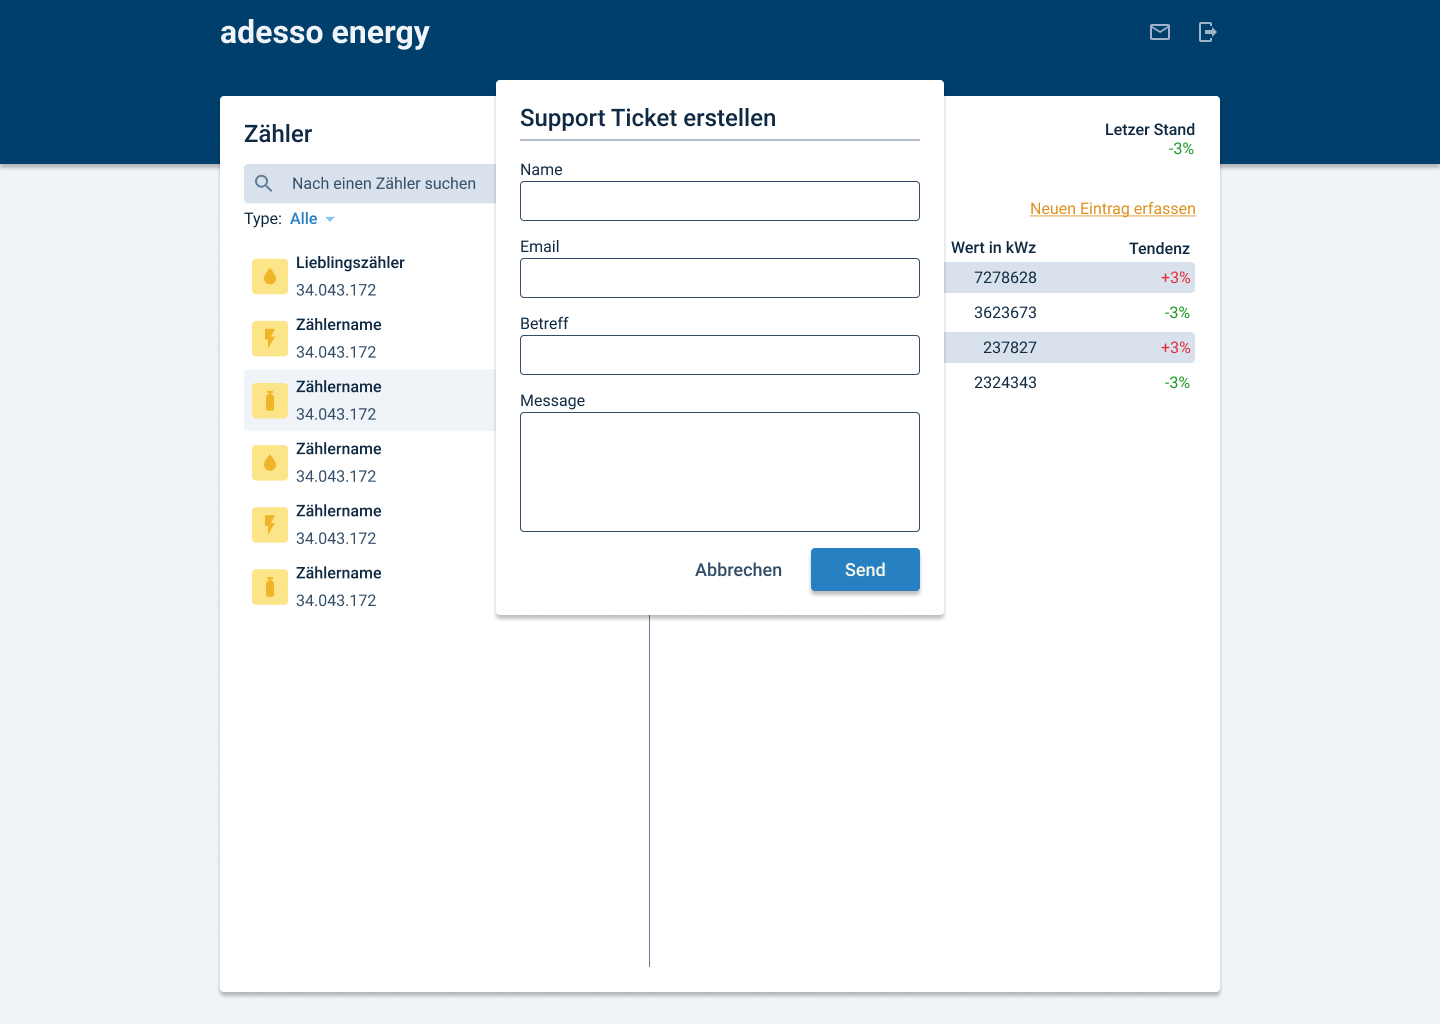
\includegraphics[scale=0.3]{img/WebsiteMockup/Dashboard-User-Mail}
	\caption{Dashboard User Support} \hfill \break
	Durch klicken auf das Mail Icon oben rechts auf der Seite wird ein Dialog zum erstellen eines neuen Support Tickets angezeigt.
\end{figure}

\newpage

\begin{figure}[h]
	\centering
    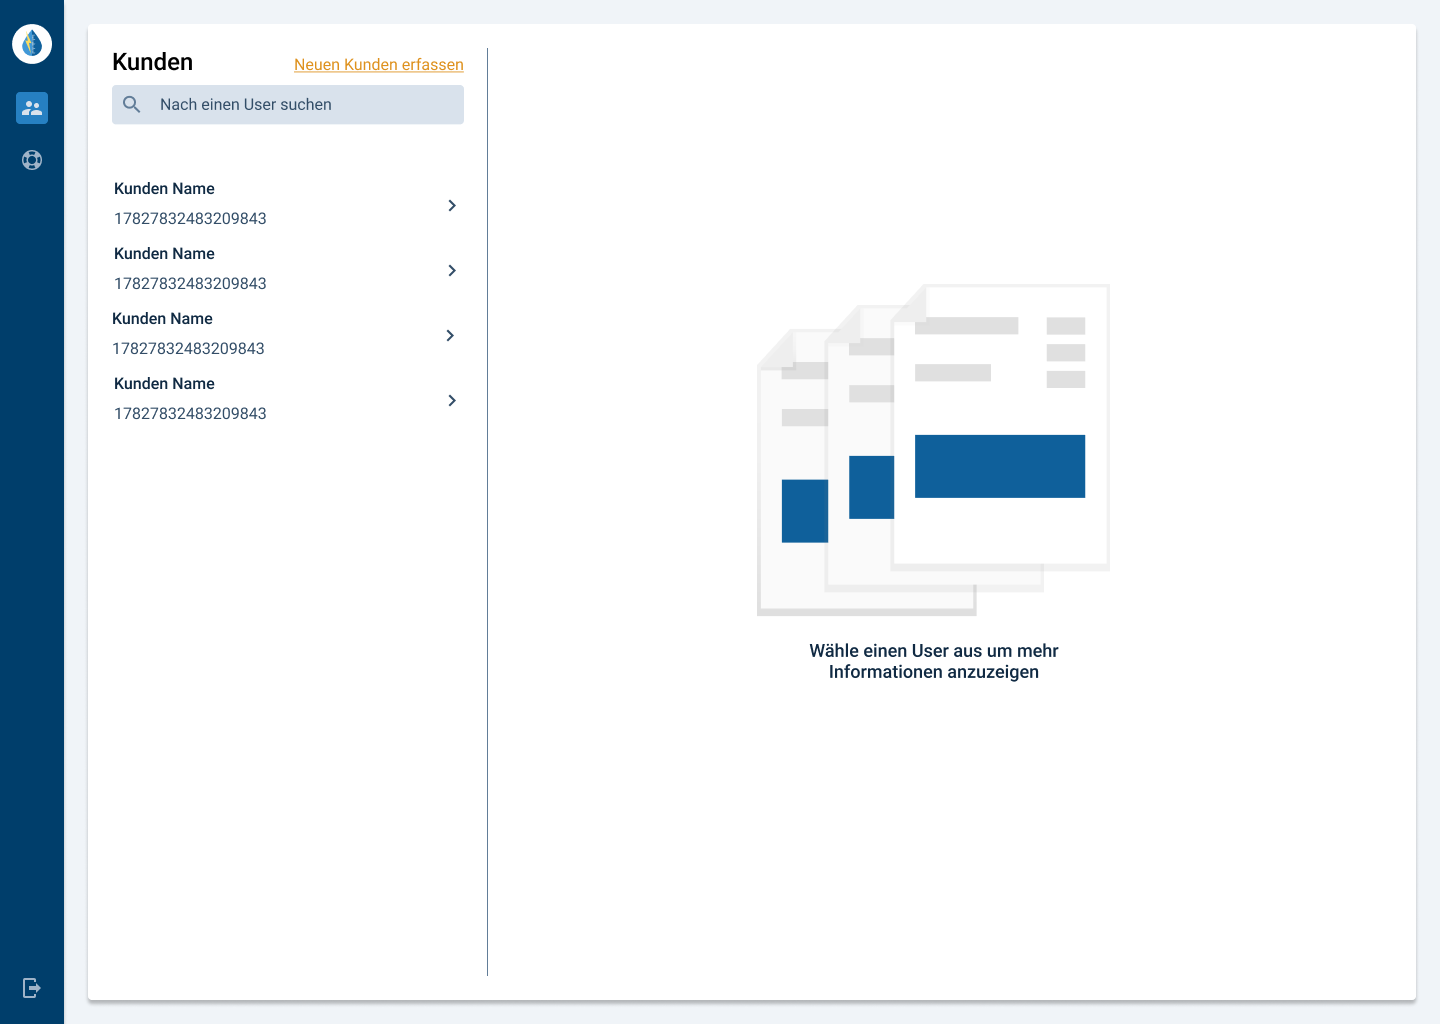
\includegraphics[scale=0.3]{img/WebsiteMockup/Dashboard-Admin-NonSelected}
	\caption{Dashboard Admin} \hfill \break
	Nachdem Login hat ein Administrator die Möglichkeit alle Kunden einzusehen.
\end{figure}

\newpage

\begin{figure}[h]
	\centering
    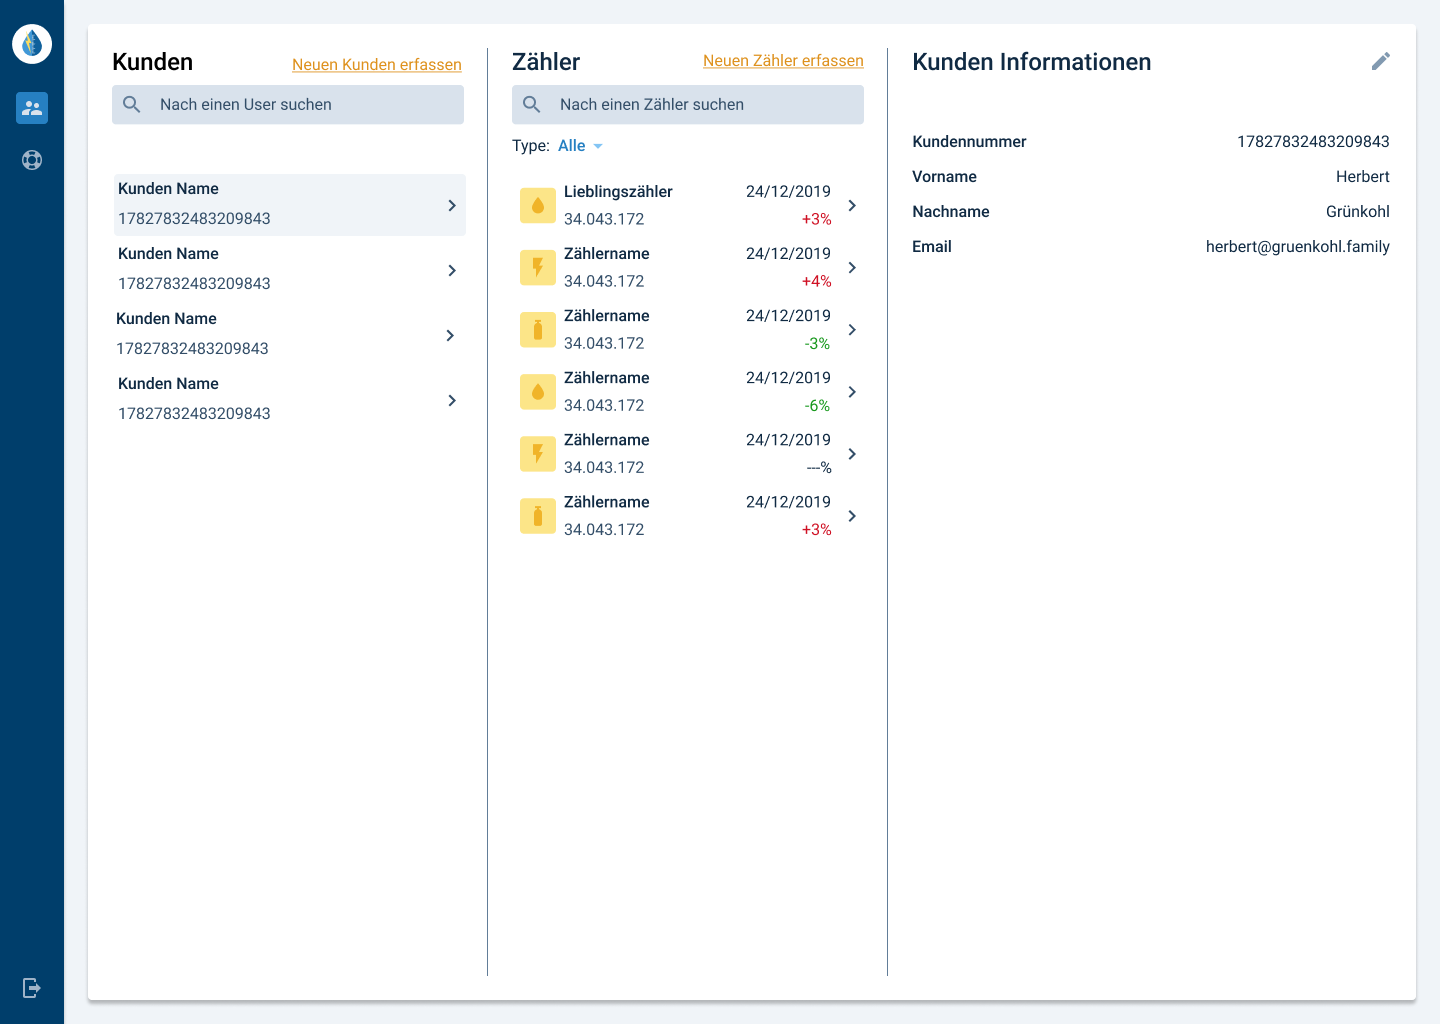
\includegraphics[scale=0.3]{img/WebsiteMockup/Dashboard-Admin-UserSelected}
	\caption{Dashboard Admin Benutzer ausgewählt} \hfill \break
	Nachdem der Administrator einen Kunden ausgewählt hat kann er die Informationen des Kunden einsehen.
\end{figure}

\newpage

\begin{figure}[h]
	\centering
    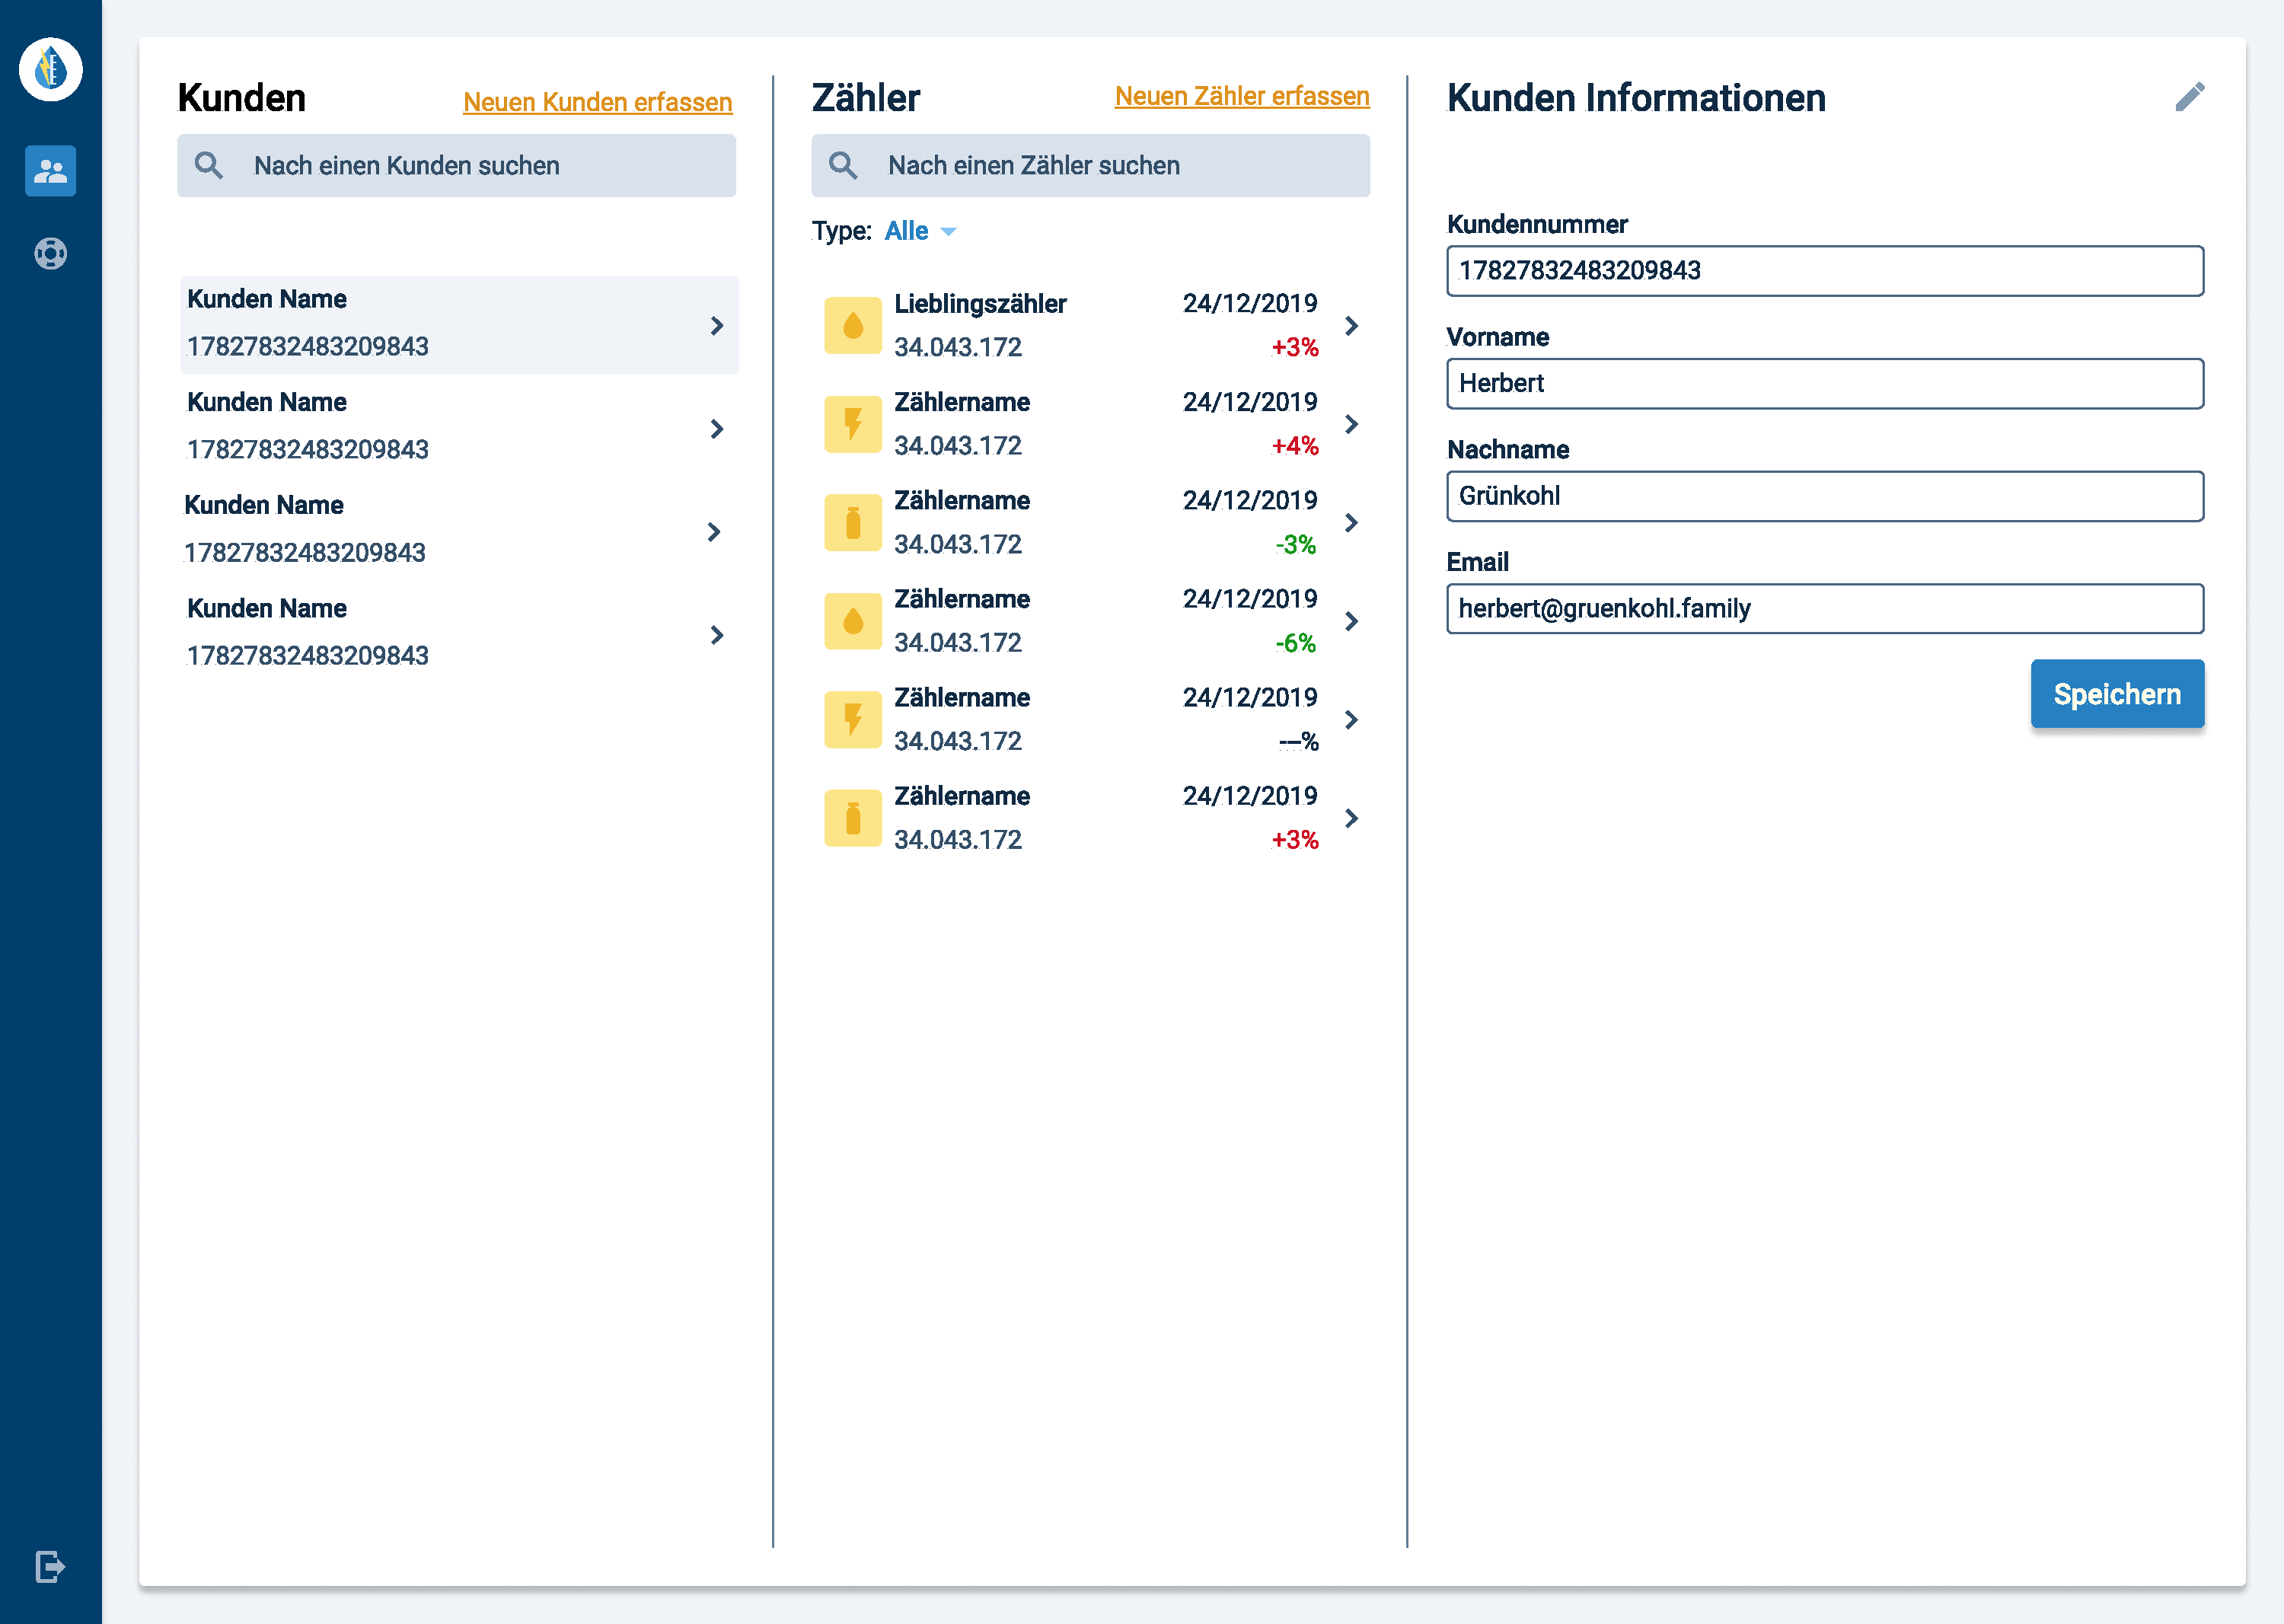
\includegraphics[scale=0.3]{img/WebsiteMockup/Dashboard-Admin-UserSelected-Edit}
	\caption{Dashboard Admin Benutzer editieren}\hfill \break
	Durch klicken des Stift Icons oben rechts auf der Seite kann ein Administrator den ausgewählten Kunden bearbeiten.
\end{figure}
\newpage

\begin{figure}[h]
	\centering
    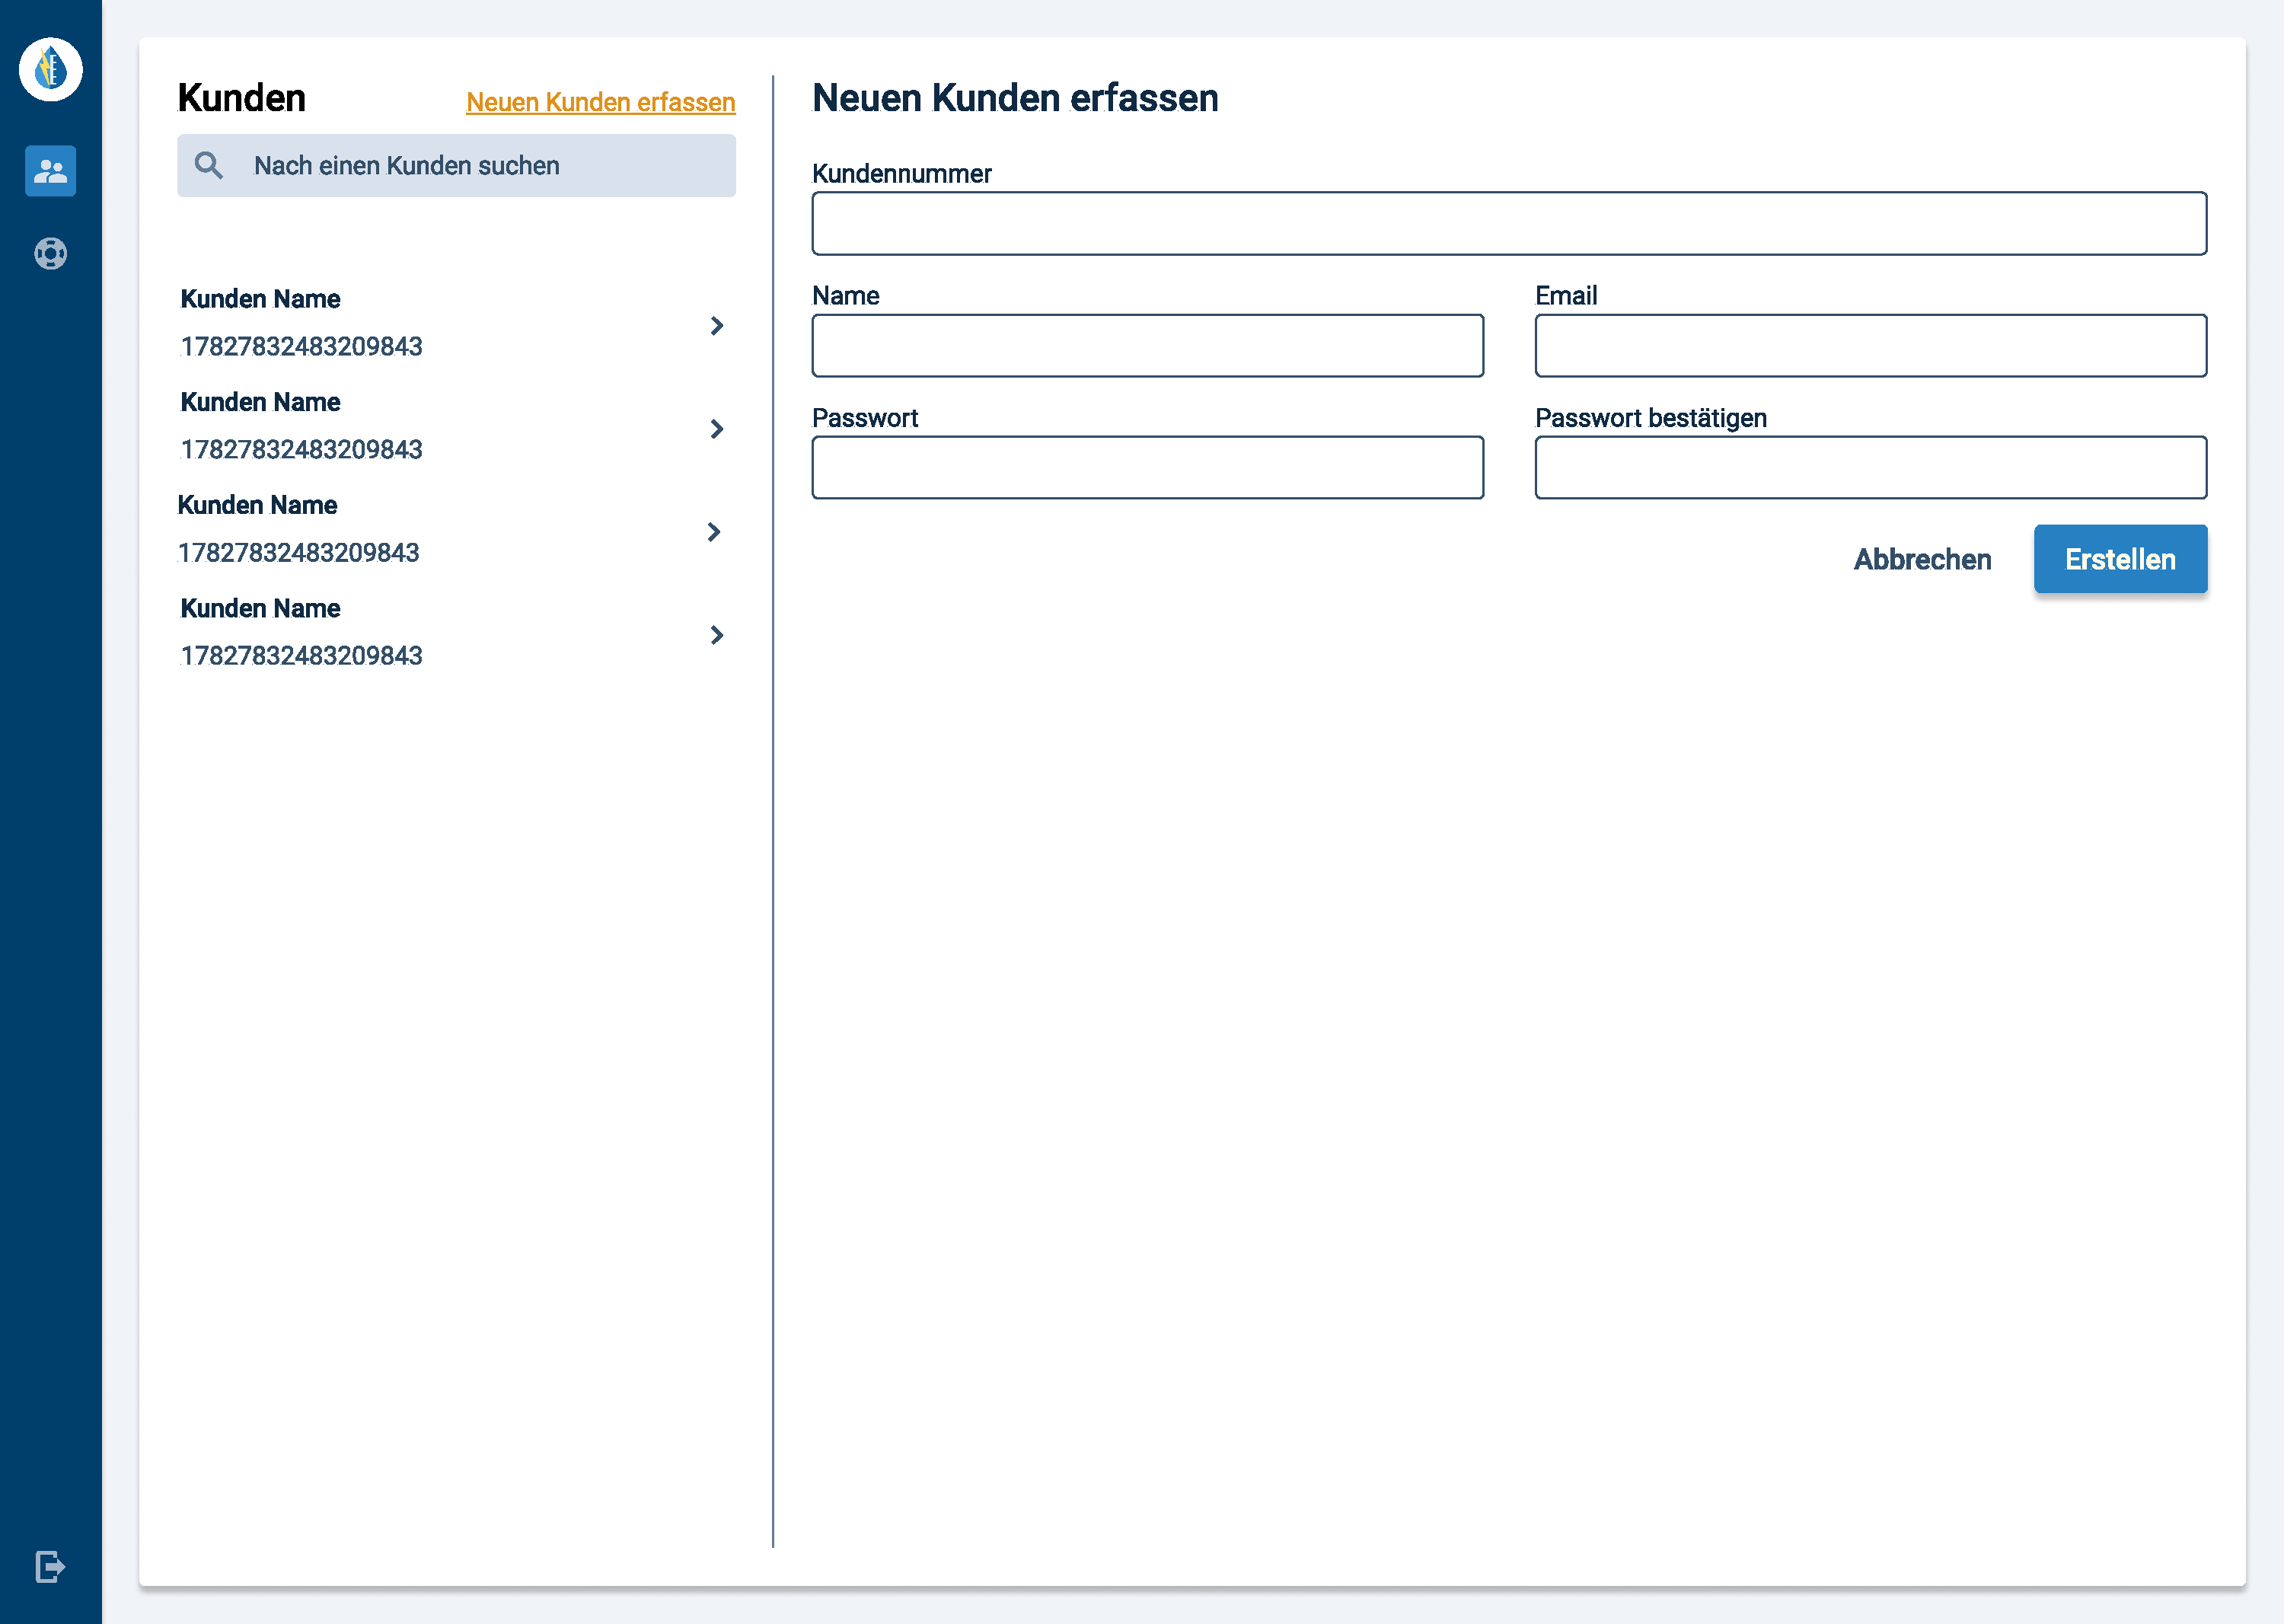
\includegraphics[scale=0.3]{img/WebsiteMockup/Dashboard-Admin-AddUser}
	\caption{Dashboard Admin Benutzer hinzufügen} \hfill \break
	Durch klicken auf Neuen Kunden erfassen kann der Administrator einen neuen Kunden zur Datenbank hinzufügen.
\end{figure}

\newpage

\begin{figure}[h]
	\centering
    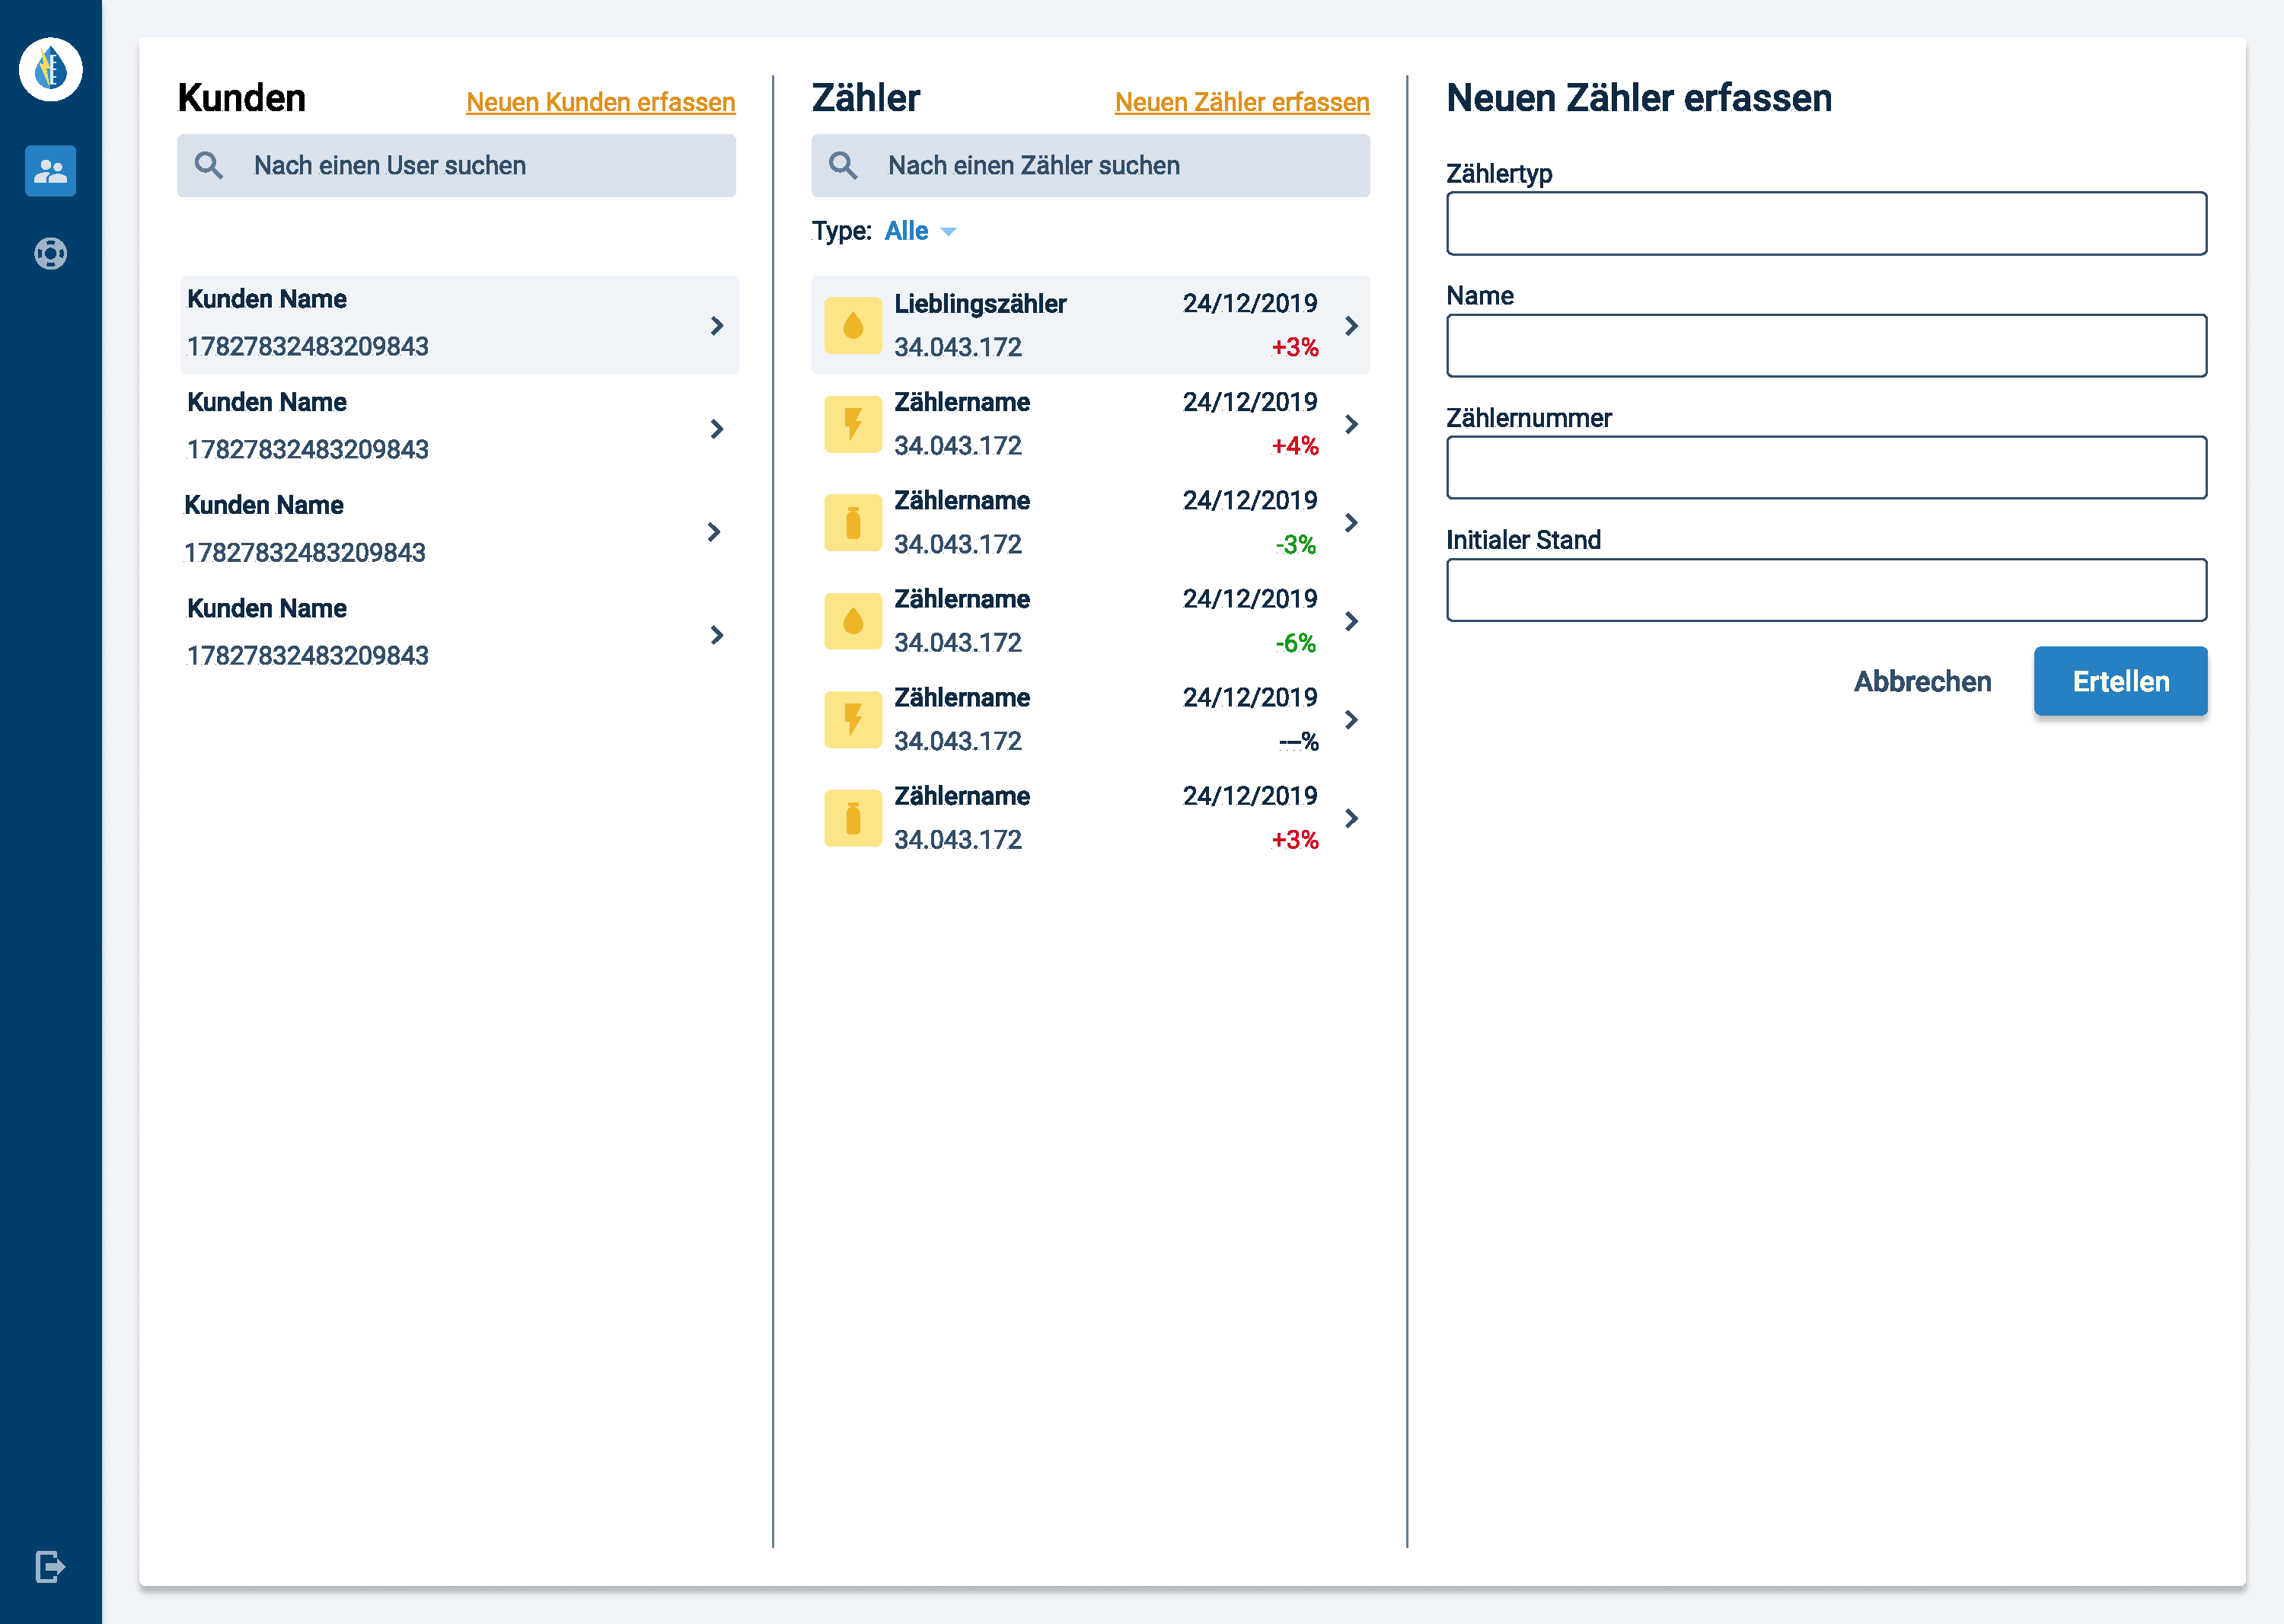
\includegraphics[scale=0.3]{img/WebsiteMockup/Dashboard-Admin-AddZahler}
	\caption{Dashboard Admin Zähler hinzufügen} \hfill \break
	Nachdem der Administrator einen Benutzer ausgewählt hat, kann er diesem einen neuen Zähler hinzufügen, indem er auf Neuen Zähler erfassen klickt.
\end{figure}

\newpage

\begin{figure}[h]
	\centering
    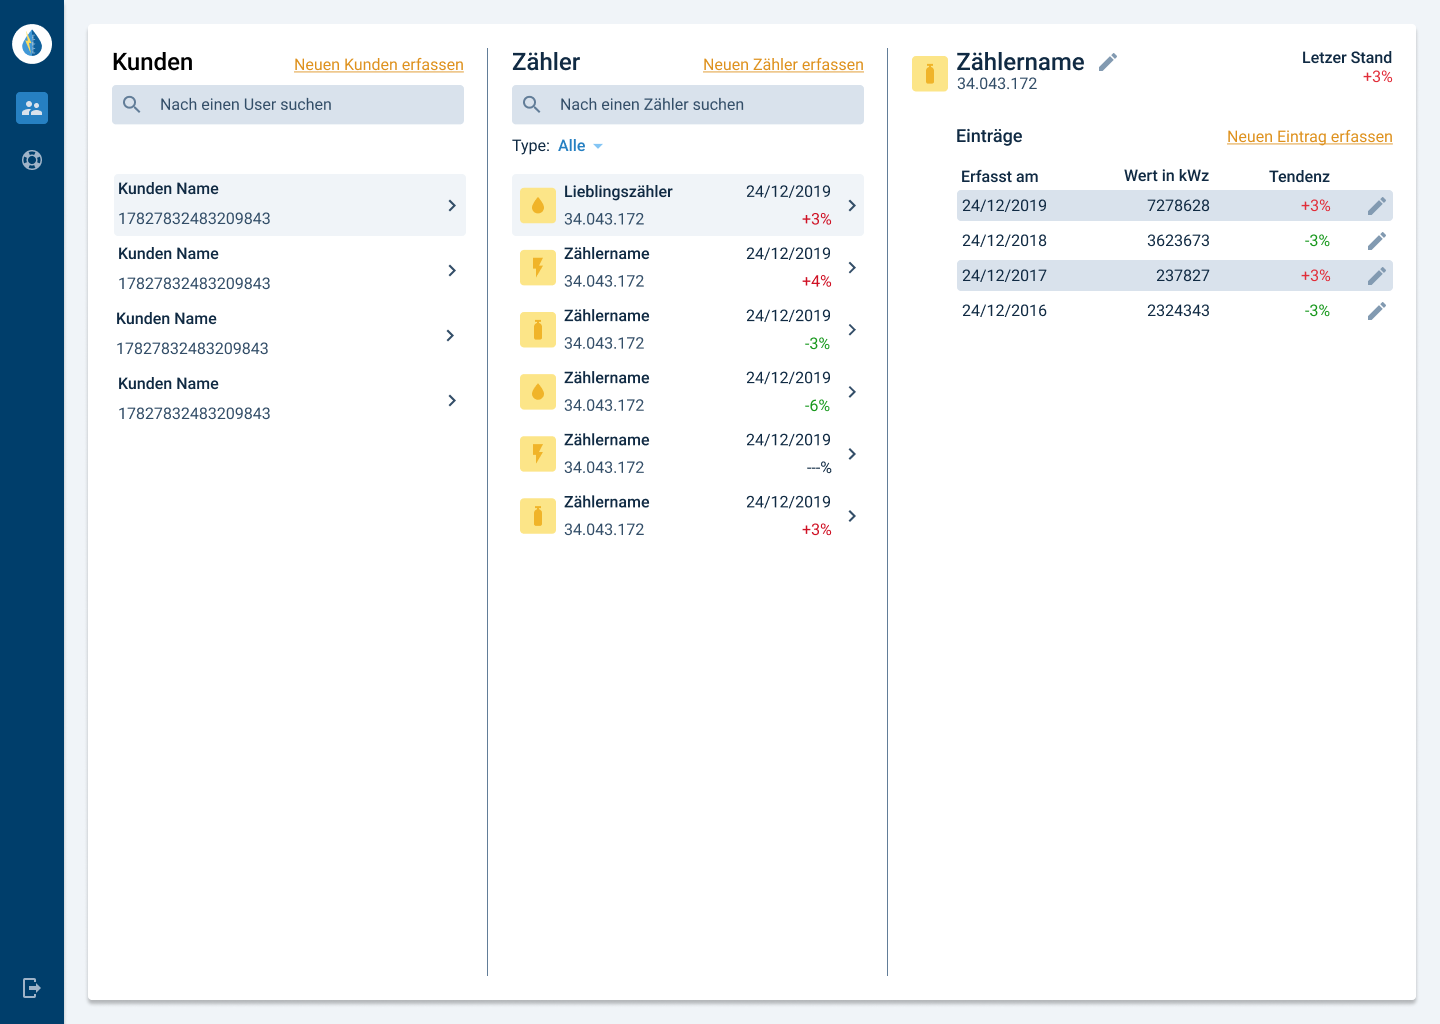
\includegraphics[scale=0.3]{img/WebsiteMockup/Dashboard-Admin-ZahlerSelected}
	\caption{Dashboard Admin Zähler ausgewählt} \hfill \break
	Nachdem der Adnimistrator auf einen Zähler geklickt hat, sieht er die Zählerinformation und History.
\end{figure}

\newpage

\begin{figure}[h]
	\centering
    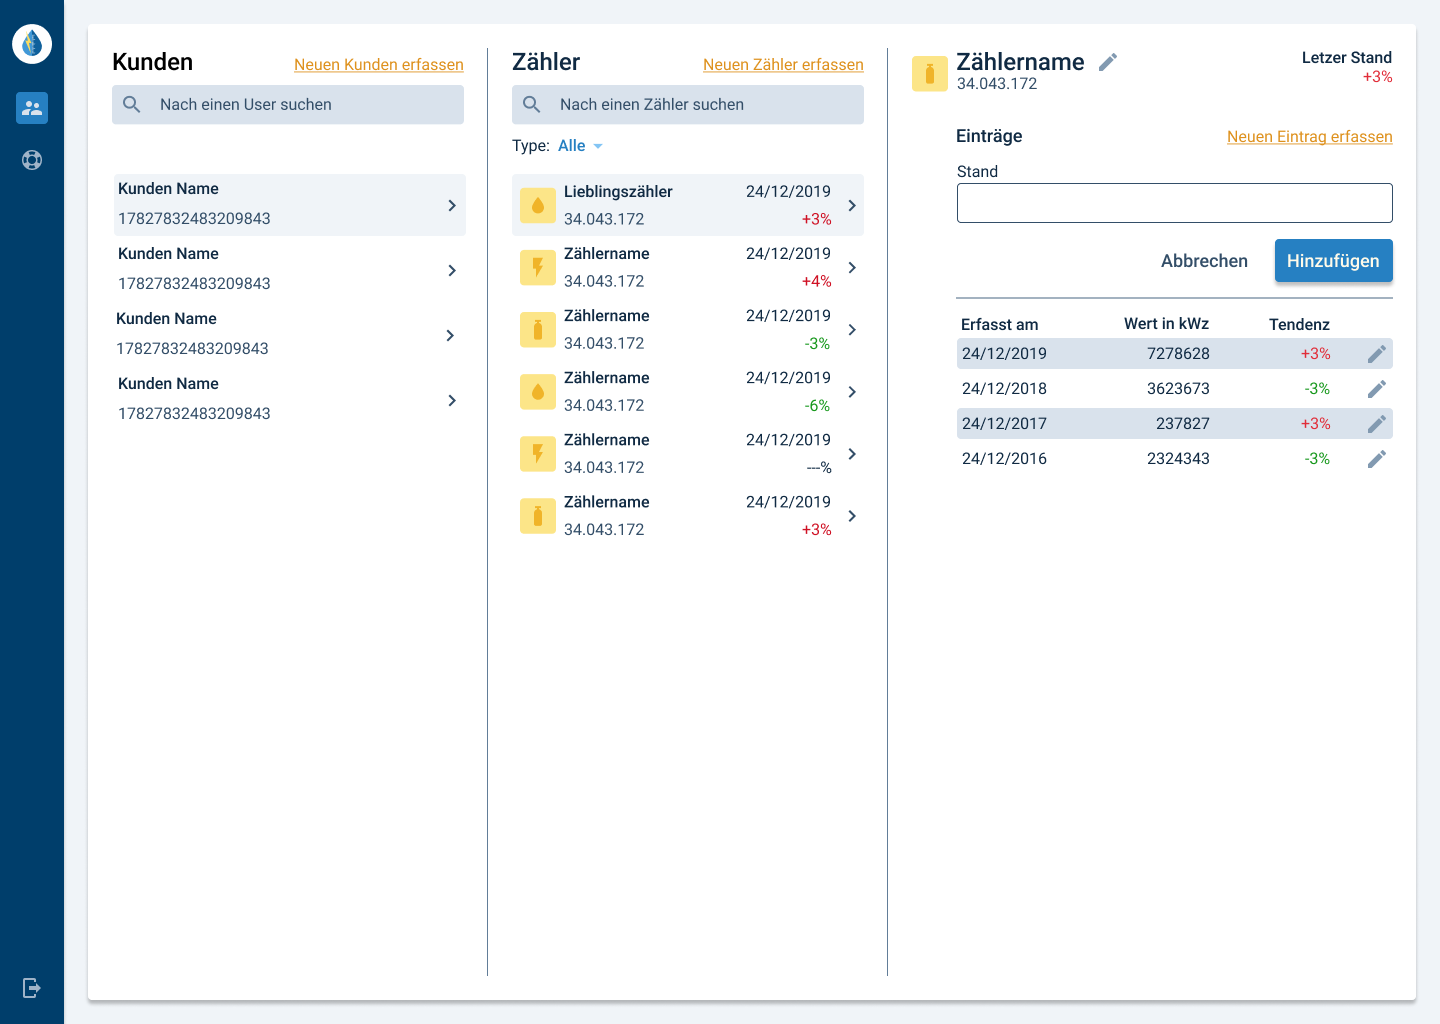
\includegraphics[scale=0.3]{img/WebsiteMockup/Dashboard-Admin-AddEntry}
	\caption{Dashboard Admin Eintrag hinzufügen} \hfill \break
	Wie auch der Benutzer hat der Admin auch die Möglichkeit Zählerstände einzutragen.
\end{figure}

\newpage

\begin{figure}[h]
	\centering
    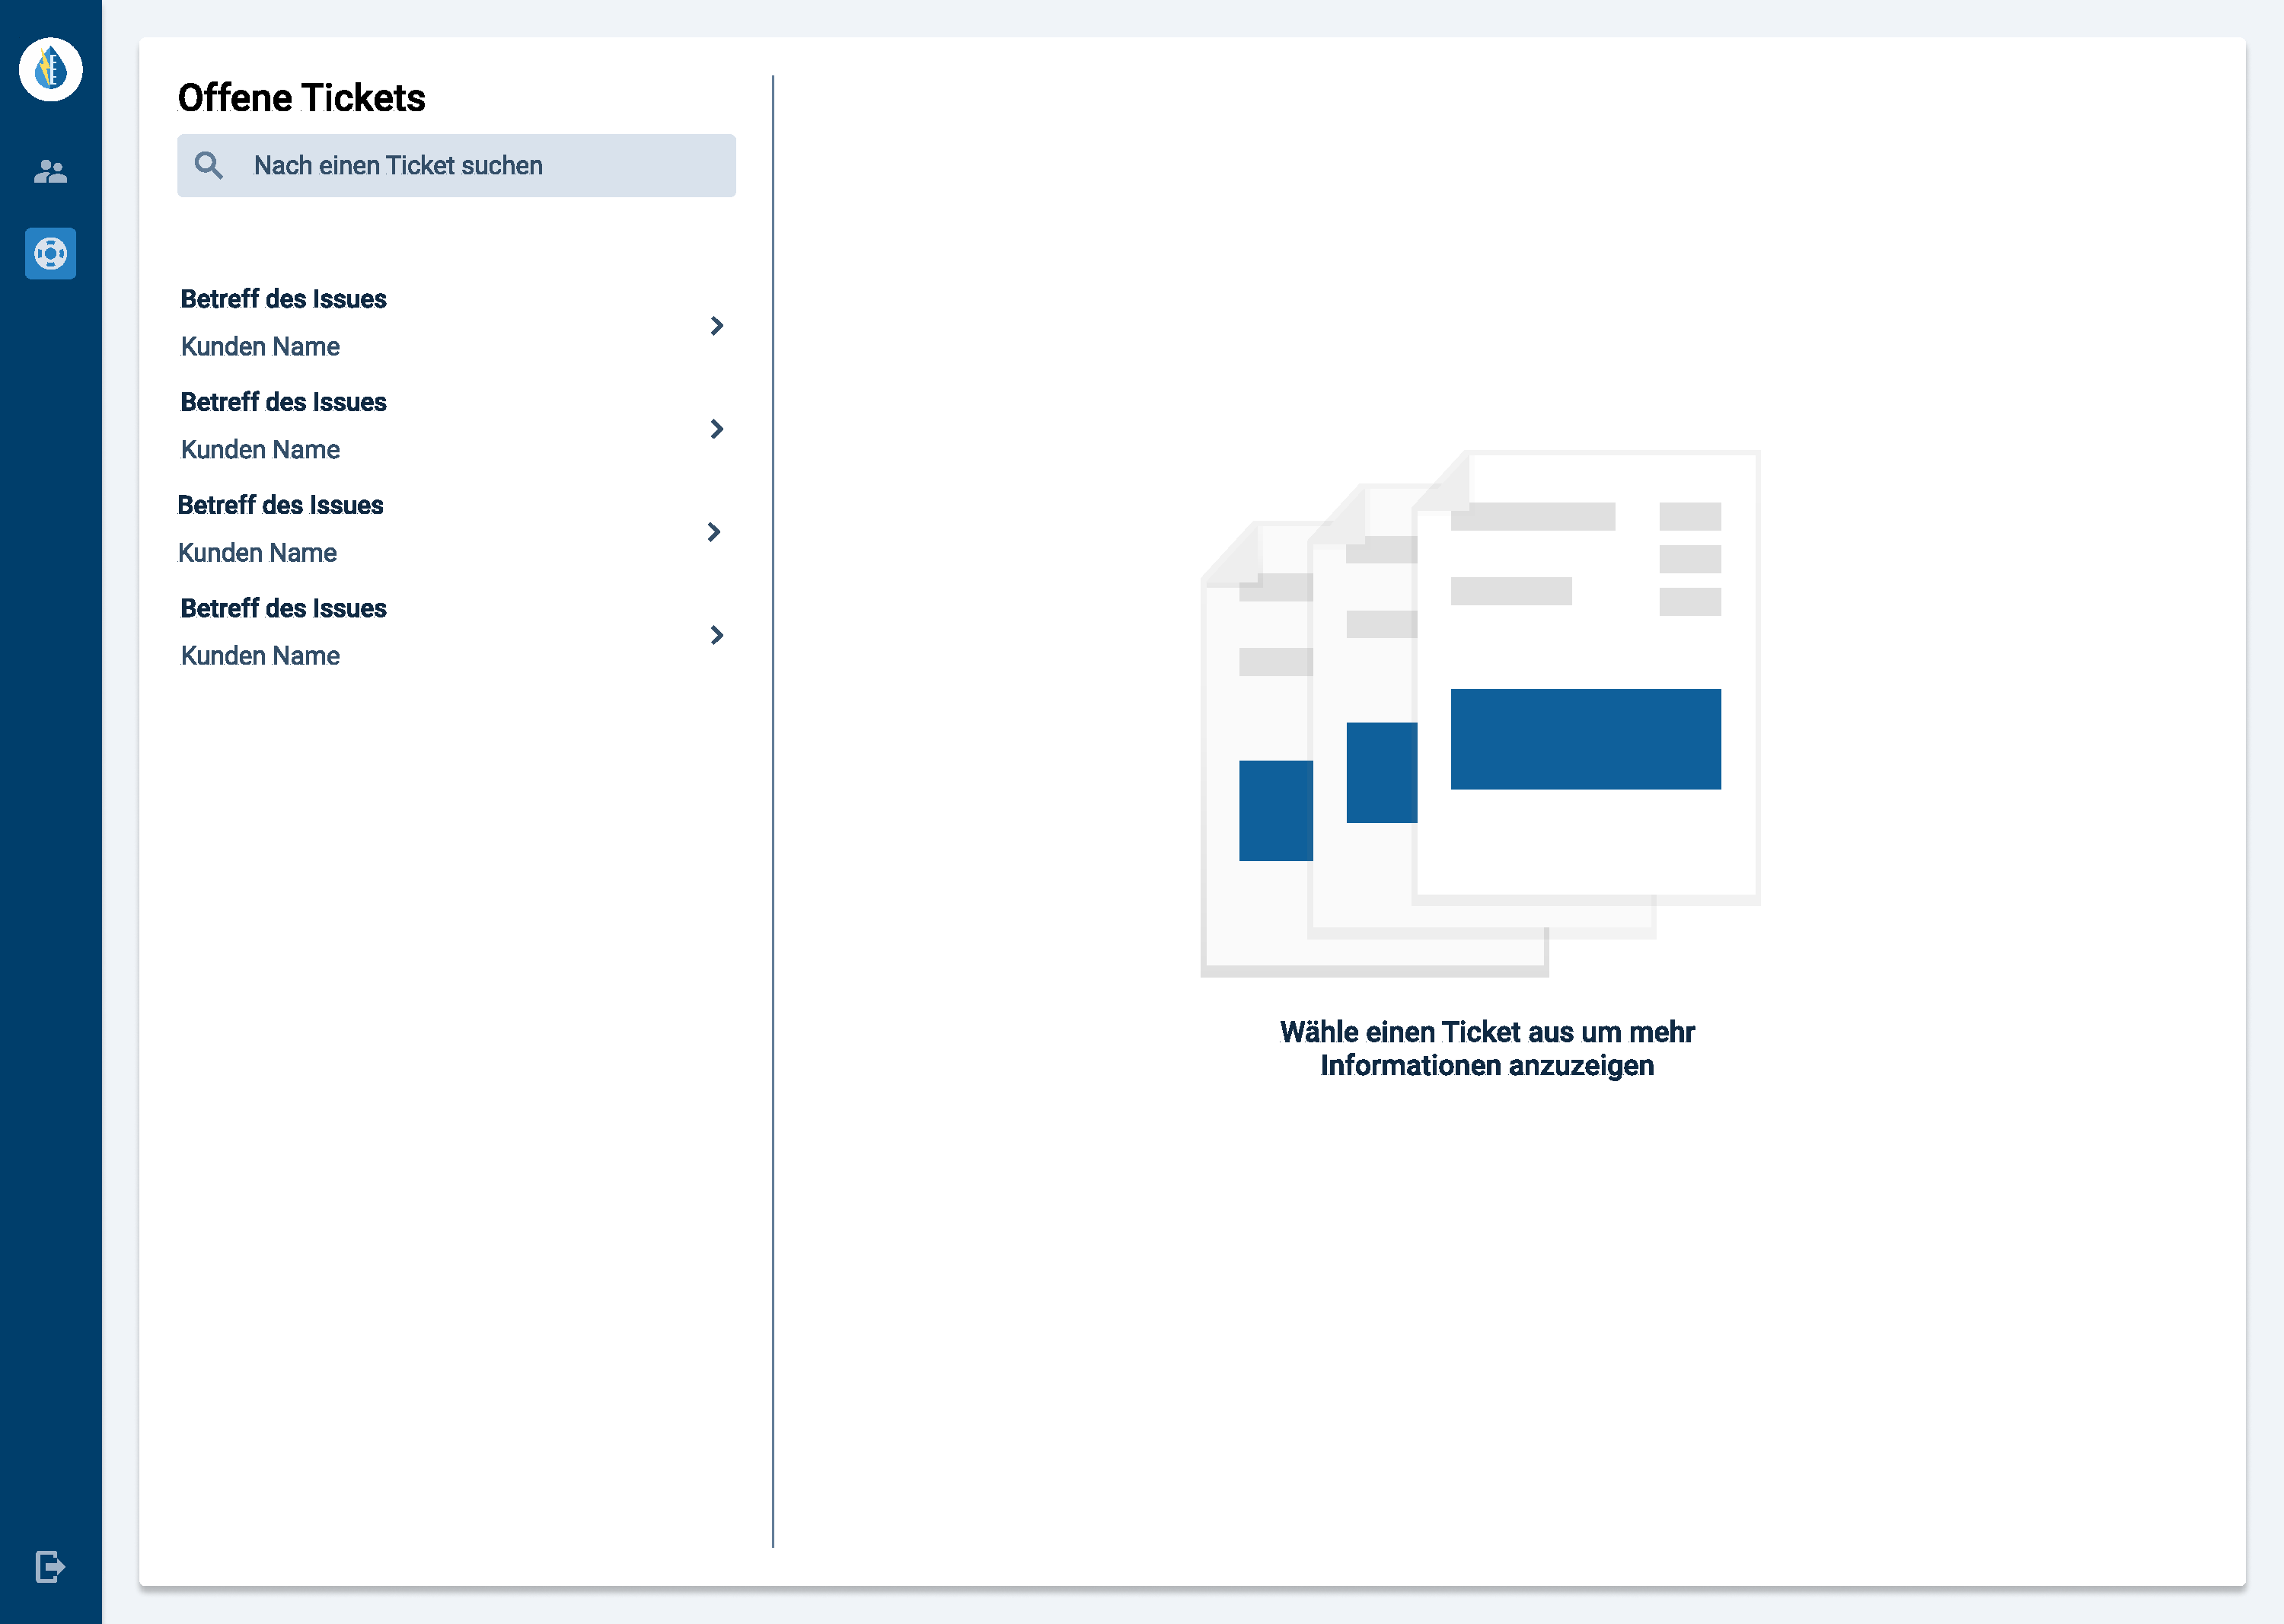
\includegraphics[scale=0.3]{img/WebsiteMockup/Dashboard-Admin-Support}
	\caption{Dashboard Admin Support} \hfill \break
	Nach dem klicken auf das Support Icon am linken Rand der Seite kann ein Administrator alle offenen Support Tickets einsehen.
\end{figure}

\newpage

\begin{figure}[h]
	\centering
    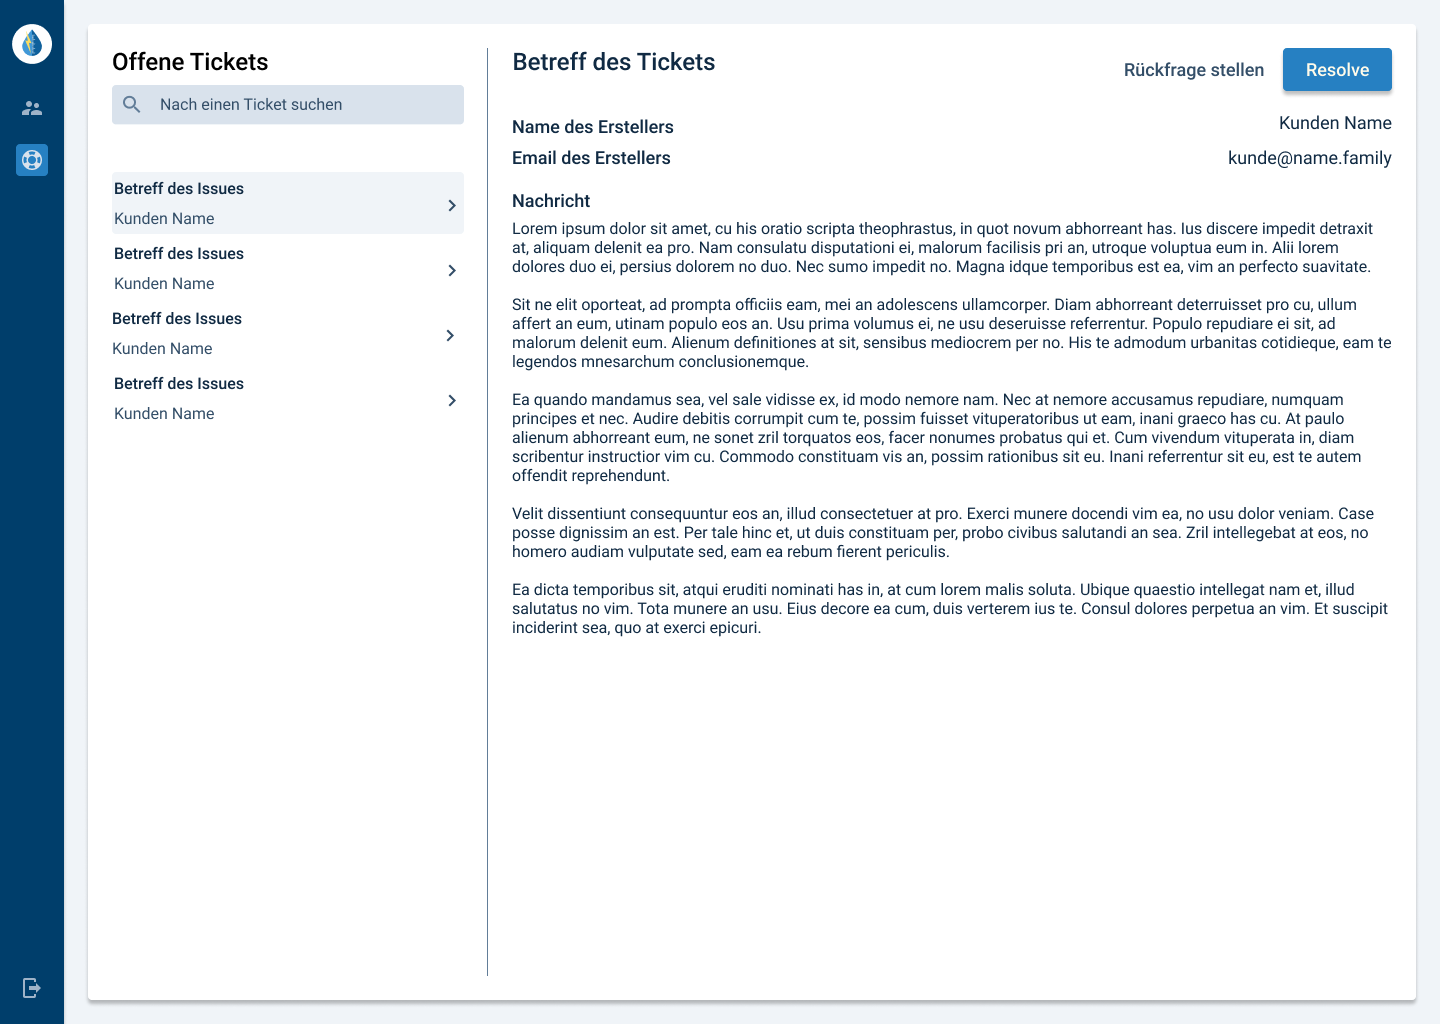
\includegraphics[scale=0.3]{img/WebsiteMockup/Dashboard-Admin-Support-Selected}
	\caption{Dashboard Admin Support Ticket ausgewählt} \hfill \break
	Durch auswählen einen Tickets kann der Administrator alle Information über das Ticket einsehen, das Ticket schließen, oder Rückfragen stellen.
\end{figure}


	
	\chapter{Glossar}\label{chp:glossar}
	\begin{table}[h]
	\centering
	\begin{tabularx}{\textwidth}{X X}
		\rowcolor[HTML]{C0C0C0} 
		\textbf{Abkürzung} & \textbf{Beschreibung} \\
		Zähler & Bei einem Zähler handelt es sich um einen Gas-, Strom- oder Wasserzähler. Er misst den Verbrauch der jeweils namensgebenden Ressource. \\
		\rowcolor[HTML]{E7E7E7} 
		FAB (Floating Action Button) & Ein FAB ist ein Knopf, der in der unteren rechten Ecke einer Android-App sitzt und Zugriff zu essentiellen Funktionen ermöglicht. \\
		Administrator (Admin) & Der Administrator, vornehmlich ein Mitarbeiter von adesso energy, hat übergeordnete Zugriffsrechte, die es ihm erlauben, auf alle Daten zuzugreifen, sowie diese zu ändern. Er interagiert hierfür ausschließlich mit der Website. \\
		\rowcolor[HTML]{E7E7E7} 
		Benutzer (User) & Als Benutzer werden Kunden von adesso energy bezeichnet. Sie haben die Möglichkeit, über die App oder Website auf ihre Nutzerdaten zuzugreifen und aktuelle Zählerstände hochzuladen. Dabei bietet die App die Option, einen Zählerstand automatisch aus einem Bild zu erkennen. Der Benutzer kann sowohl mit der App als auch mit der Website interagieren. \\
		Web-Applikation & Der Server ist nicht Teil einer Web-Applikation. Aufgrund der umfassenden React-Architektur betrachten wir die Website als eigene Applikation. \\
		\rowcolor[HTML]{E7E7E7} 
		DTO (data transfer object) & Als data transfer objects bezeichnen wir die Objekte, die unsere Anwendungen über das HTTP-Protokoll übertragen. \\
		Paging & Durch paging  wird beschränkt, wie viele Daten ein Server auf einmal an einen Client versendet. 
	\end{tabularx}
	\caption{Glossar}
	\label{table:glossar}
\end{table}
	
	\bibliography{references}
	\pagenumbering{gobble} % Nummerierung deaktivieren
	
\end{document}
